\documentclass[12pt,a4paper]{report}

\usepackage[utf8]{inputenc}
\usepackage[T1]{fontenc}
\usepackage[french]{babel}
\usepackage{graphicx}
\usepackage{geometry}
\usepackage{hyperref}
\usepackage{fancyhdr}
\usepackage{setspace}
\usepackage{float}
\geometry{margin=2.5cm}
\onehalfspacing

\pagestyle{fancy}
\fancyhf{}
\fancyfoot[C]{\thepage}

\begin{document}

%=================================================
% PAGE DE GARDE
%=================================================
\begin{titlepage}

\begin{center}

\vspace*{0.5cm}

%--------------------------------------------------
% Logo entreprise
%--------------------------------------------------

\includegraphics[width=0.22\textwidth]{image/logo_entreprise.jpg}

\vspace{1.8cm}

%--------------------------------------------------
% Titre principal
%--------------------------------------------------
{\Huge\bfseries Documentation Technique}

\vspace{0.3cm}

\rule{0.85\textwidth}{1pt}

\vspace{0.4cm}

{\Large Développement et Intégration d'une Solution}

\vspace{0.4cm}

\rule{0.85\textwidth}{1pt}

\vspace{2.5cm}

%--------------------------------------------------
% Titre de la tâche
%--------------------------------------------------
\fbox{
\begin{minipage}{0.80\textwidth}
\centering
\vspace{0.5cm}
{\LARGE\bfseries Grille Fonctionnelle}
\vspace{0.5cm}
\end{minipage}
}

\vspace{3cm}

%--------------------------------------------------
% Informations
%--------------------------------------------------
\renewcommand{\arraystretch}{2}

\begin{tabular}{|p{6cm}|p{6cm}|}
\hline

\centering\textbf{Réalisé par} &
\centering\textbf{Entreprise}
\tabularnewline

\hline

\centering Maha El Allam &
\centering Smart Holol
\tabularnewline

\hline

\end{tabular}

\vfill

%--------------------------------------------------
% Pied de page
%--------------------------------------------------
\rule{\textwidth}{0.6pt}

\vspace{0.5cm}

{\large Documentation de réalisation}

\vspace{0.3cm}

{\large Juin 2026}

\end{center}

\end{titlepage}

%=================================================
% SOMMAIRE
%=================================================
\tableofcontents
\newpage

%=================================================
% INTRODUCTION
%=================================================
\chapter*{Introduction Générale}
\addcontentsline{toc}{chapter}{Introduction Générale}

Le présent document détaille l'architecture, la méthodologie de conception et les protocoles d'intégration de la solution technique déployée pour répondre aux impératifs opérationnels de \textbf{Smart Holol}. Dans un contexte où l'optimisation des processus métiers est devenue un levier stratégique de performance, cette réalisation s'inscrit dans une démarche de structuration et de fiabilisation de l'écosystème informatique de l'entreprise.

L'objectif central de ce projet est de concevoir une réponse technique pérenne, scalable et alignée avec les standards de qualité de l'organisation. À travers l'analyse fonctionnelle détaillée dans la \textit{Grille Fonctionnelle}, ce guide expose les fondements technologiques adoptés, les choix d'implémentation et les étapes de configuration critique. 

Au-delà de la description des fonctionnalités, ce document sert de référentiel technique complet. Il a été conçu pour assurer la continuité opérationnelle, faciliter la maintenance corrective et servir de socle évolutif pour les futures itérations du projet. Il permet ainsi une lecture transverse, tant pour les parties prenantes souhaitant comprendre la logique métier que pour les équipes techniques chargées de la pérennisation et de l'optimisation continue de la solution.

%=================================================
% CONTEXTE
%=================================================
\chapter{Contexte de la tâche}

\section{Présentation du besoin}

Dans le secteur des agences de voyage, la gestion des activités commerciales, administratives et opérationnelles implique le traitement d'un grand nombre d'informations relatives aux clients, aux prestataires, aux réservations et aux dossiers de voyage. L'utilisation de plusieurs outils distincts pour gérer ces processus peut entraîner des pertes de temps, des erreurs de saisie et des difficultés de suivi.

Afin de centraliser l'ensemble des processus métiers, une solution basée sur \textbf{Odoo Community} a été mise en place. Cette solution permet d'intégrer au sein d'une plateforme unique la gestion de la relation client (CRM), des ventes, des achats, de la facturation, des dossiers de voyage, du site web et des ressources humaines.

Cette documentation présente les différentes étapes de configuration et d'utilisation des modules mis en œuvre afin de répondre aux exigences de la grille fonctionnelle et d'assurer une gestion intégrée, cohérente et efficace des activités de l'agence de voyage.

\section{Objectifs}

Les principaux objectifs de cette réalisation sont les suivants :

\begin{itemize}
    \item Centraliser la gestion des données clients et des prospects.
    \item Automatiser les processus commerciaux, depuis la demande de devis jusqu'à la facturation.
    \item Faciliter le suivi des dossiers de voyage et des tâches administratives.
    \item Améliorer la collaboration entre les différents services de l'entreprise.
    \item Mettre à disposition un site web permettant la présentation des offres, la réservation en ligne et l'accès à un espace client sécurisé.
    \item Fournir des outils d'analyse permettant de suivre les performances commerciales.
    \item Réduire les traitements manuels et améliorer la traçabilité des opérations.
\end{itemize}

\section{Résultat attendu}

À l'issue de cette réalisation, l'entreprise dispose d'un système d'information intégré permettant de gérer l'ensemble du cycle de vie d'un dossier client, depuis la prise de contact jusqu'au suivi après-vente.

La solution mise en place permet notamment :

\begin{itemize}
    \item la gestion centralisée des prospects et des opportunités commerciales ;
    \item la création et le suivi des devis, commandes et factures ;
    \item la gestion des fournisseurs et des prestations de voyage ;
    \item la génération automatique des dossiers de voyage ;
    \item la publication des offres sur le site web et la réservation en ligne ;
    \item la mise à disposition d'un espace client sécurisé ;
    \item la planification des activités et la gestion des ressources humaines ;
    \item le suivi des indicateurs commerciaux grâce aux tableaux de bord d'Odoo.
\end{itemize}

Cette documentation constitue également un guide technique destiné à faciliter le déploiement, la maintenance et les évolutions futures de la solution.

%=================================================
% PREREQUIS
%=================================================
\chapter{Prérequis}

\section{Logiciels nécessaires}

La mise en œuvre de la solution nécessite les logiciels suivants :

\begin{itemize}
    \item Odoo Community ;
    \item PostgreSQL ;
    \item Python (environnement d'exécution d'Odoo) ;
    \item Git ;
    \item Visual Studio Code ;
    \item Un navigateur web moderne (Google Chrome, Mozilla Firefox ou Microsoft Edge).
\end{itemize}

\section{Technologies utilisées}

Les principales technologies utilisées dans ce projet sont :

\begin{itemize}
    \item Odoo Community ;
    \item Python ;
    \item PostgreSQL ;
    \item XML (vues et configuration Odoo) ;
    \item HTML, CSS et JavaScript pour les composants du site web ;
    \item QWeb pour les modèles de documents générés par Odoo.
\end{itemize}

\section{Configuration requise}

La solution a été développée et testée dans l'environnement suivant :

\begin{itemize}
    \item Système d'exploitation : Windows 11 (ou toute distribution Linux compatible avec Odoo) ;
    \item Odoo Community ;
    \item PostgreSQL ;
    \item Python 3.x ;
    \item Mémoire vive : 8 Go minimum (16 Go recommandés) ;
    \item Navigateur web récent compatible avec Odoo.
\end{itemize}

%=================================================
% REALISATION
%=================================================

%=================================================
% MODULE CRM
%=================================================
\chapter{Module CRM}
\section{GESTION DES PROSPECTS \& DEMANDES}

\subsection{Capture automatique des demandes de devis de voyage depuis le site internet}

Le module \textbf{Website} couplé au module \textbf{CRM} d'Odoo permet de transformer automatiquement les demandes envoyées depuis un formulaire de contact du site web en pistes commerciales (\textit{Leads}) ou en opportunités dans le pipeline CRM.

Pour configurer cette fonctionnalité, accéder au module \textbf{Site Web}.

\begin{figure}[H]
\centering
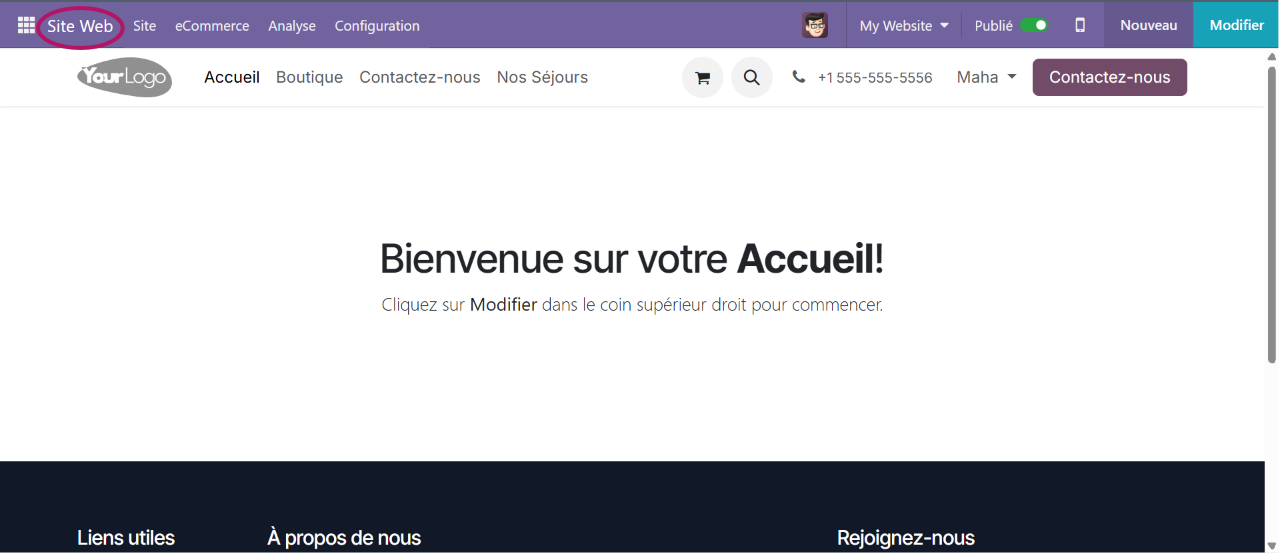
\includegraphics[width=\linewidth]{image/CRM/CRM1.png}
\caption{Accès au module Site Web}
\label{fig:crm1}
\end{figure}

Ouvrir ensuite la page sur laquelle le formulaire de contact doit être ajouté.

\begin{figure}[H]
\centering
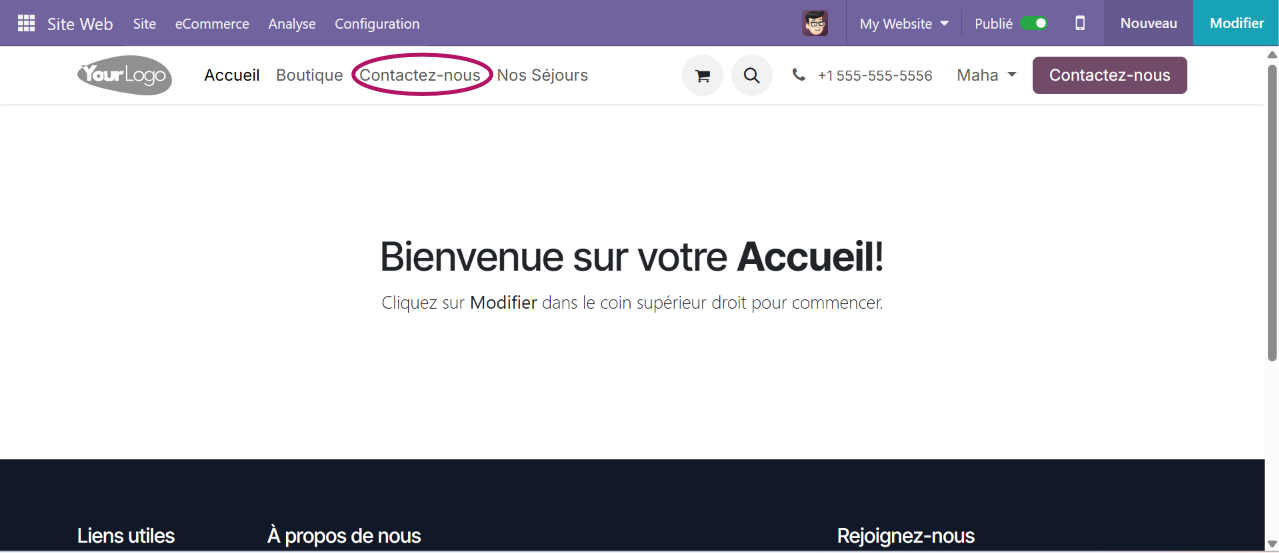
\includegraphics[width=\linewidth]{image/CRM/CRM2.png}
\caption{Page du site web}
\label{fig:crm2}
\end{figure}

Cliquer sur le bouton \textbf{Modifier} afin de passer en mode édition.

\begin{figure}[H]
\centering
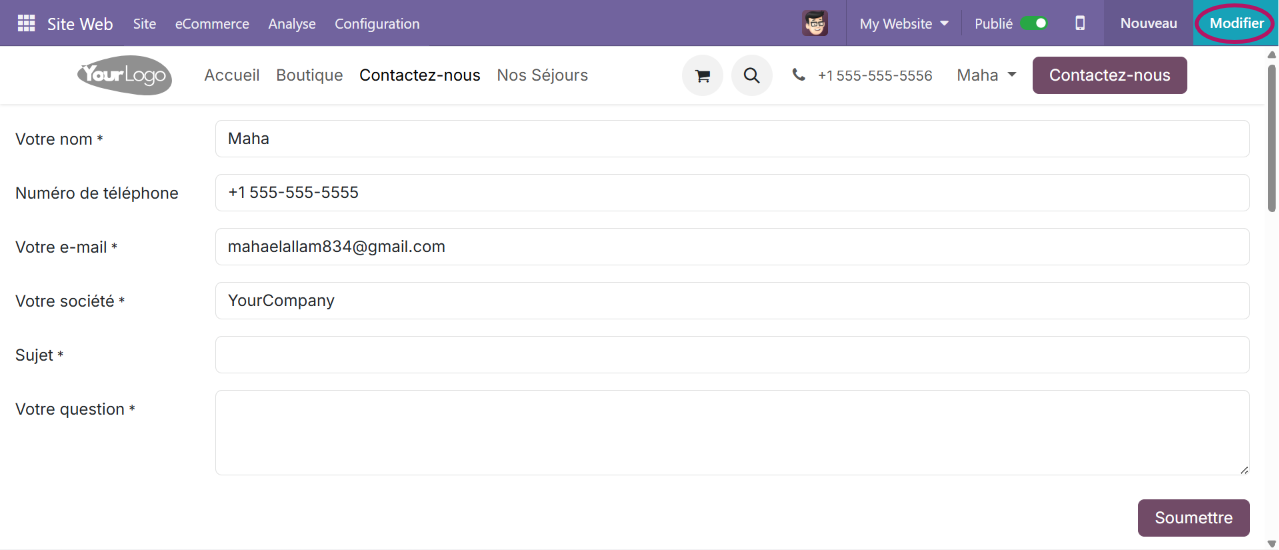
\includegraphics[width=\linewidth]{image/CRM/CRM3.png}
\caption{Activation du mode édition}
\label{fig:crm3}
\end{figure}

Dans l'onglet \textbf{Blocs}, puis dans la catégorie \textbf{Contenu interne}, sélectionner le bloc \textbf{Formulaire} et le faire glisser sur la page.

\begin{figure}[H]
\centering
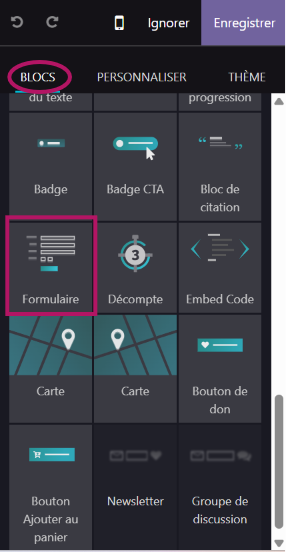
\includegraphics{image/CRM/CRM4.png}
\caption{Ajout du bloc Formulaire}
\label{fig:crm4}
\end{figure}

Sélectionner ensuite le formulaire afin de personnaliser son contenu. Les champs peuvent être ajoutés, supprimés ou modifiés selon les informations à collecter (nom, e-mail, destination, nombre de voyageurs, dates, etc.).

\begin{figure}[H]
\centering
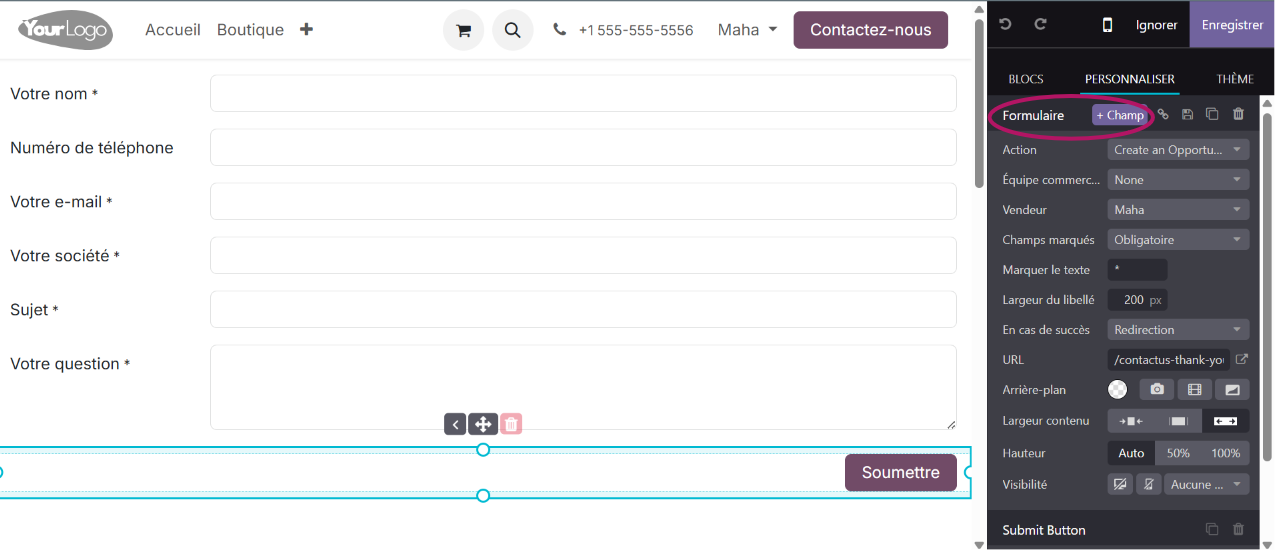
\includegraphics[width=\linewidth]{image/CRM/CRM5.png}
\caption{Personnalisation du formulaire}
\label{fig:crm5}
\end{figure}

Dans les propriétés du formulaire, définir l'action \textbf{Créer une opportunité} (\textit{Create Opportunity}) afin que chaque soumission génère automatiquement une opportunité dans le CRM.

\begin{figure}[H]
\centering
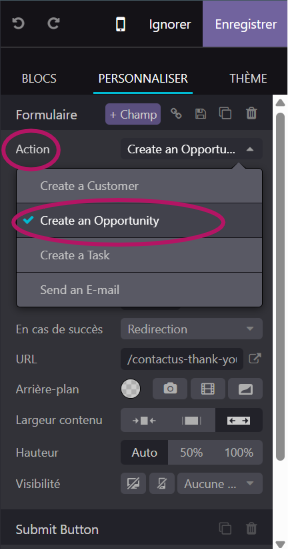
\includegraphics{image/CRM/CRM6.png}
\caption{Configuration de l'action du formulaire}
\label{fig:crm6}
\end{figure}

Il est également possible d'affecter automatiquement les opportunités créées à un commercial spécifique.

\begin{figure}[H]
\centering
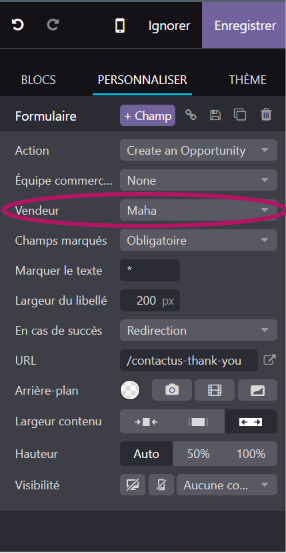
\includegraphics
{image/CRM/CRM7.png}
\caption{Affectation automatique d'un commercial}
\label{fig:crm7}
\end{figure}

Une fois la configuration terminée, enregistrer les modifications.

\begin{figure}[H]
\centering
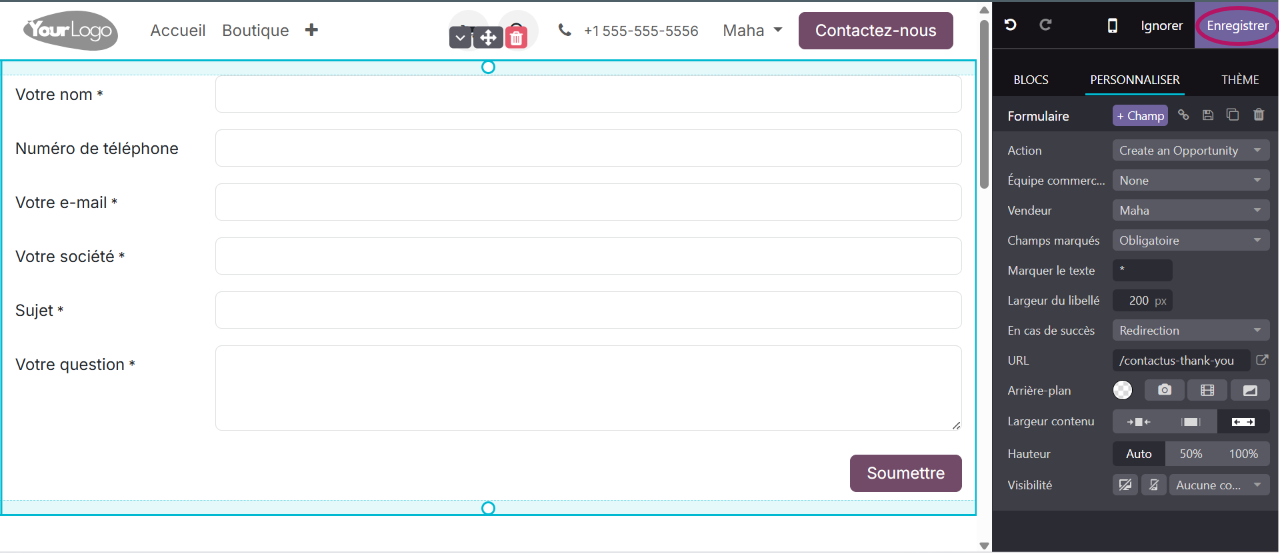
\includegraphics[width=\linewidth]{image/CRM/CRM8.png}
\caption{Enregistrement des modifications}
\label{fig:crm8}
\end{figure}

Depuis le site web, un client peut remplire le formulaire de contact et le soumettre.

\begin{figure}[H]
\centering
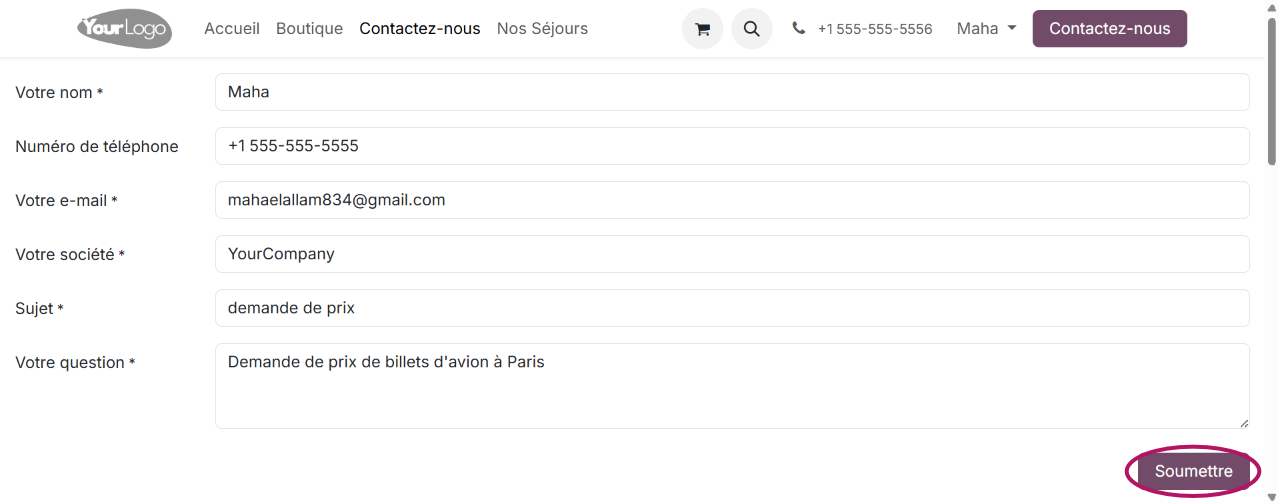
\includegraphics[width=\linewidth]{image/CRM/CRM9.png}
\caption{Soumission d'une demande }
\label{fig:crm9}
\end{figure}

Après la soumission du formulaire, accéder au module \textbf{CRM}.

\begin{figure}[H]
\centering
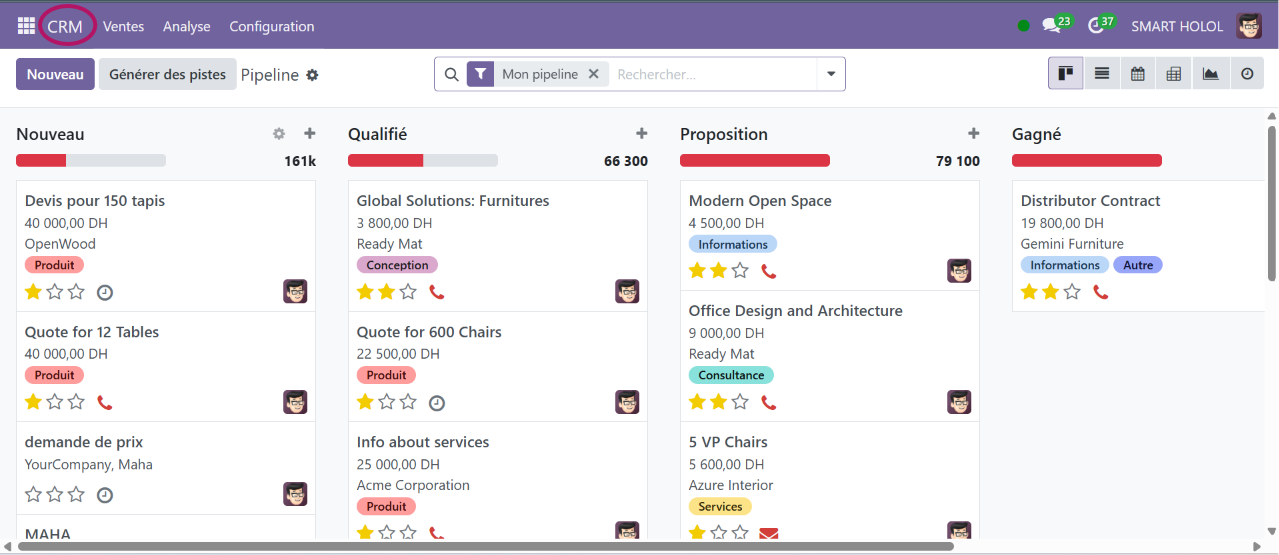
\includegraphics[width=\linewidth]{image/CRM/CRM10.png}
\caption{Accès au module CRM}
\label{fig:crm10}
\end{figure}

La demande est automatiquement créée sous forme d'une nouvelle opportunité dans le pipeline CRM, ce qui permet aux équipes commerciales de la traiter sans intervention manuelle.

\begin{figure}[H]
\centering
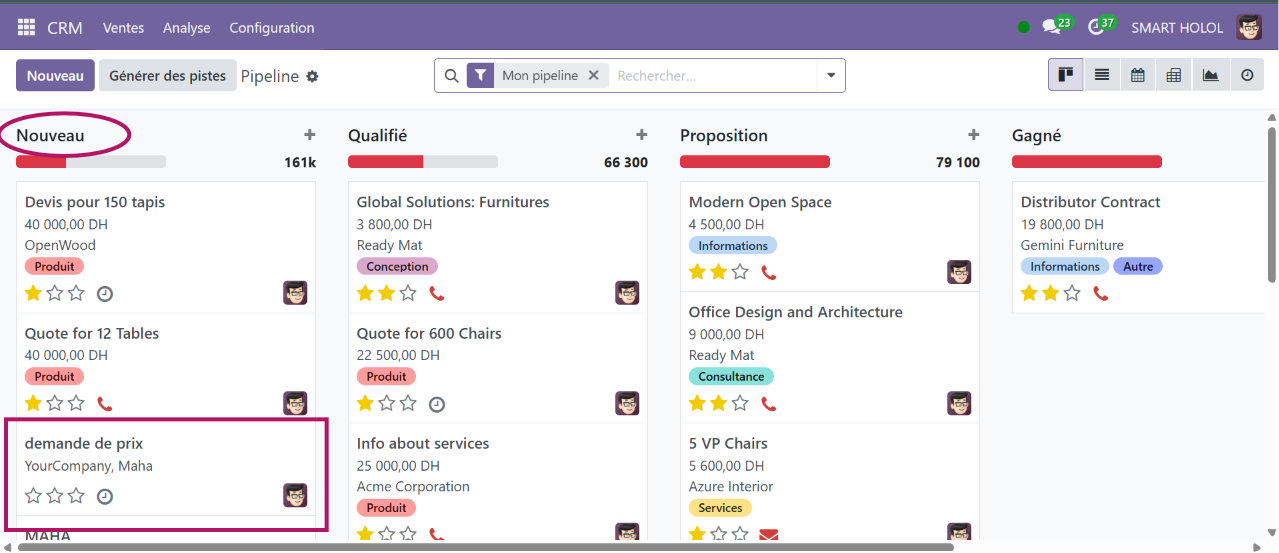
\includegraphics[width=\linewidth]{image/CRM/CRM11.png}
\caption{Nouvelle opportunité créée automatiquement dans le CRM}
\label{fig:crm11}
\end{figure}
\subsection{Qualification des préférences de voyage des prospects}

La qualification des prospects consiste à enrichir les opportunités avec des informations permettant de mieux comprendre les besoins des clients, telles que la destination souhaitée, le budget estimé, le nombre de voyageurs ou le type de séjour. Dans Odoo, cette qualification peut être réalisée à l'aide des \textbf{étiquettes (Tags)} du module CRM. Pour des besoins plus avancés, des modules communautaires de l'\textit{Odoo Community Association (OCA)} permettent d'ajouter des champs de qualification supplémentaires.

Accéder au module \textbf{CRM}.

\begin{figure}[H]
\centering
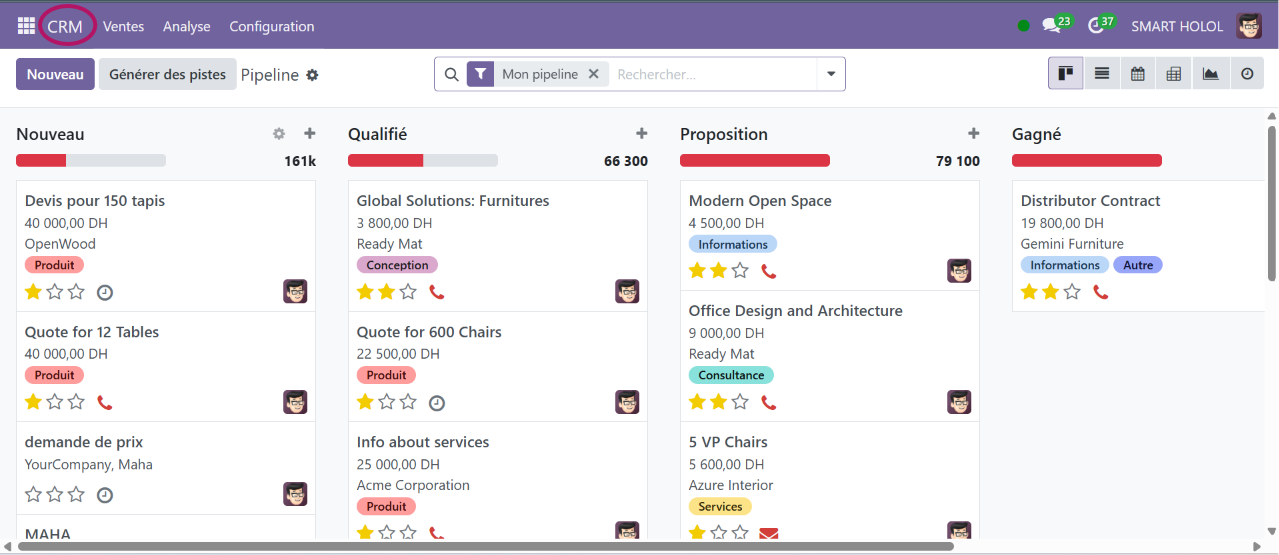
\includegraphics[width=\linewidth]{image/CRM/CRM10.png}
\caption{Accès au module CRM}
\label{fig:crm12_1}
\end{figure}

Dans le menu \textbf{Configuration}, sélectionner \textbf{Étiquettes}.

\begin{figure}[H]
\centering
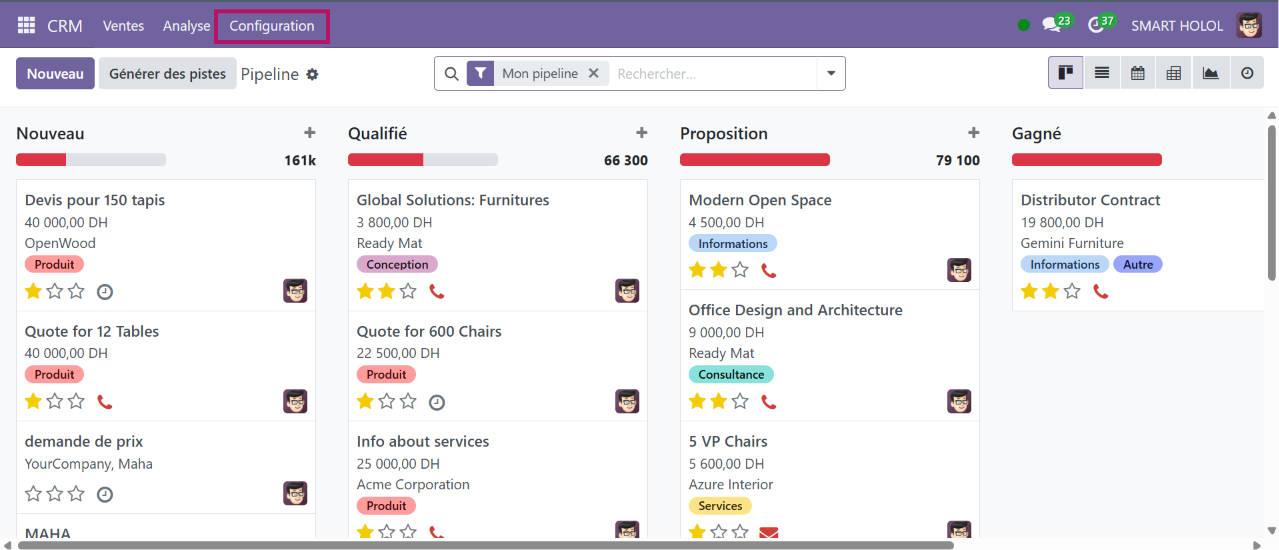
\includegraphics[width=\linewidth]{image/CRM/CRM12.png}
\caption{Menu Configuration du CRM}
\label{fig:crm12_2}
\end{figure}

La liste des étiquettes existantes s'affiche.

\begin{figure}[H]
\centering
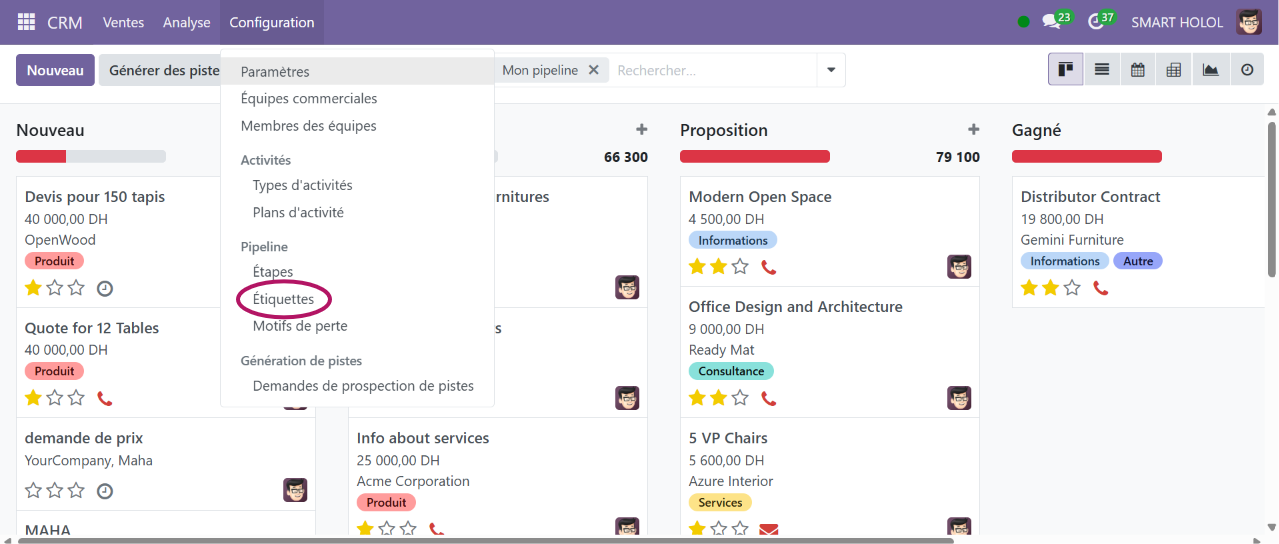
\includegraphics[width=\linewidth]{image/CRM/CRM13.png}
\caption{Liste des étiquettes CRM}
\label{fig:crm12_3}
\end{figure}

Cliquer sur le bouton \textbf{Nouveau} afin de créer une nouvelle étiquette.

\begin{figure}[H]
\centering
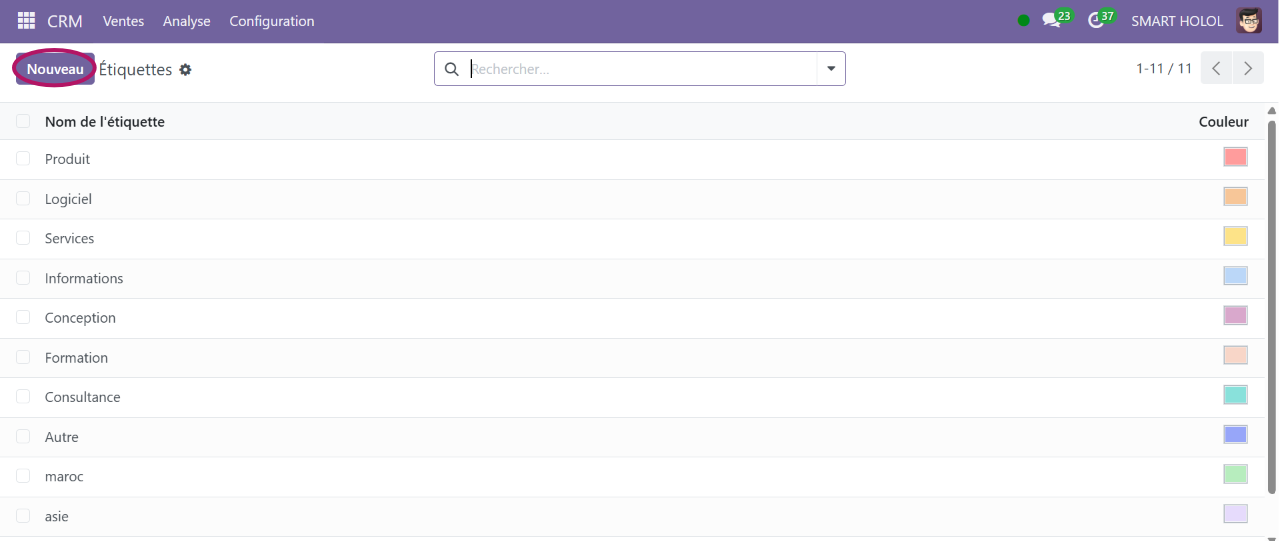
\includegraphics[width=\linewidth]{image/CRM/CRM14.png}
\caption{Création d'une nouvelle étiquette}
\label{fig:crm12_4}
\end{figure}

Renseigner le nom de l'étiquette, choisir une couleur puis enregistrer les modifications.

\begin{figure}[H]
\centering
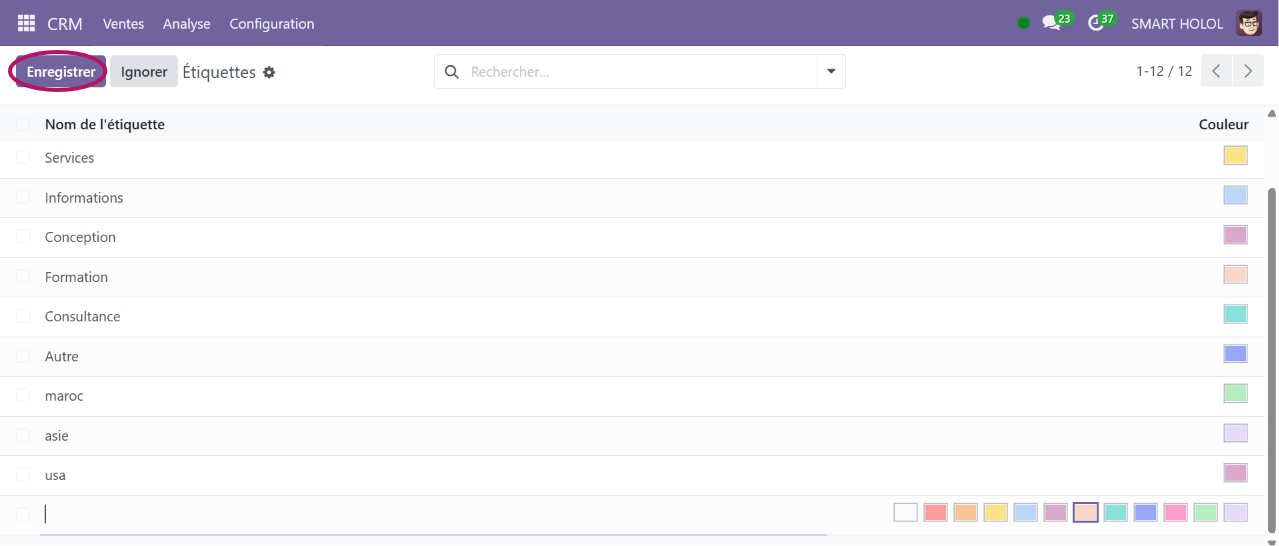
\includegraphics[width=\linewidth]{image/CRM/CRM15.png}
\caption{Configuration d'une étiquette}
\label{fig:crm12_5}
\end{figure}

Revenir ensuite au pipeline du module \textbf{CRM}.

\begin{figure}[H]
\centering
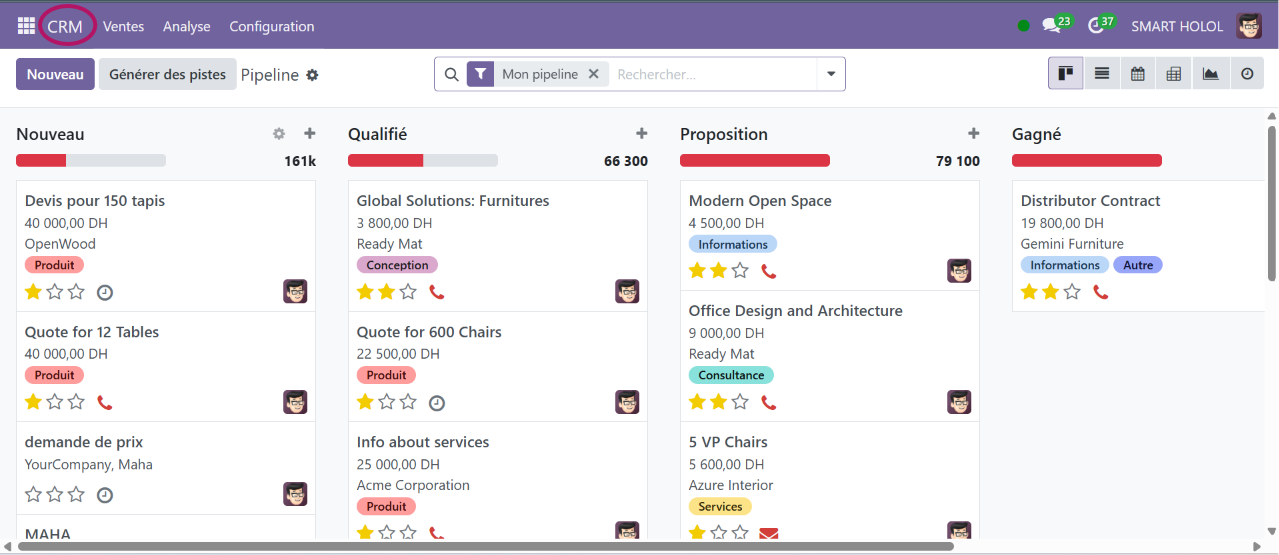
\includegraphics[width=\linewidth]{image/CRM/CRM10.png}
\caption{Retour au pipeline CRM}
\label{fig:crm12_6}
\end{figure}

Ouvrir l'opportunité concernée.

\begin{figure}[H]
\centering
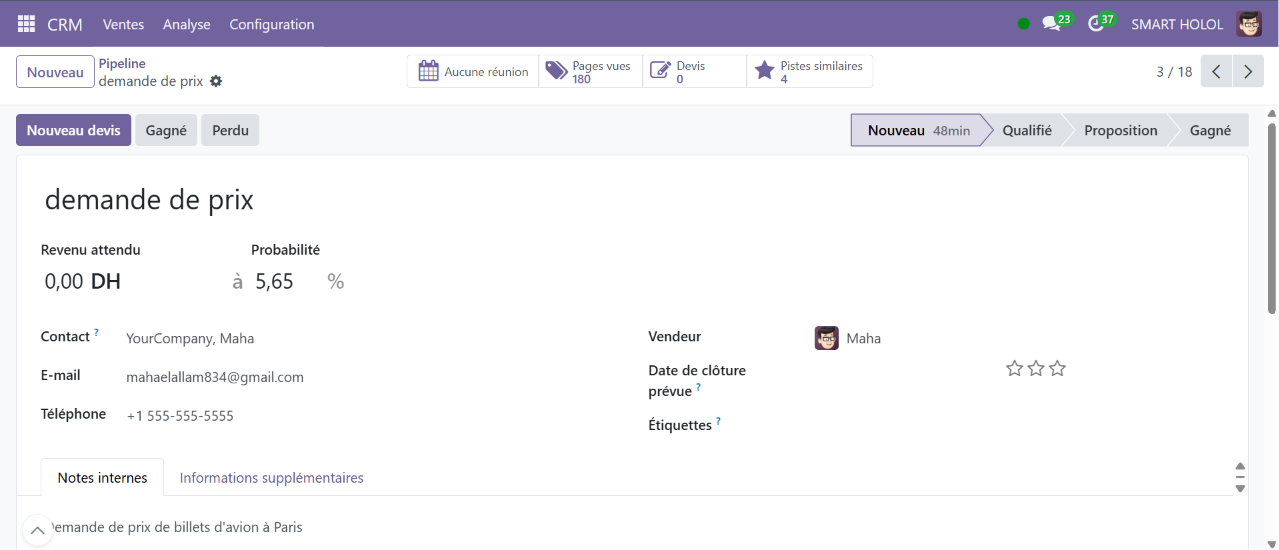
\includegraphics[width=\linewidth]{image/CRM/CRM16.png}
\caption{Ouverture d'une opportunité}
\label{fig:crm12_7}
\end{figure}

Enfin, associer les étiquettes créées à l'opportunité afin de qualifier les préférences du prospect (par exemple : \textit{Voyage en groupe}, \textit{Séjour balnéaire}, \textit{Budget élevé}, \textit{Destination Europe}, etc.).

\begin{figure}[H]
\centering
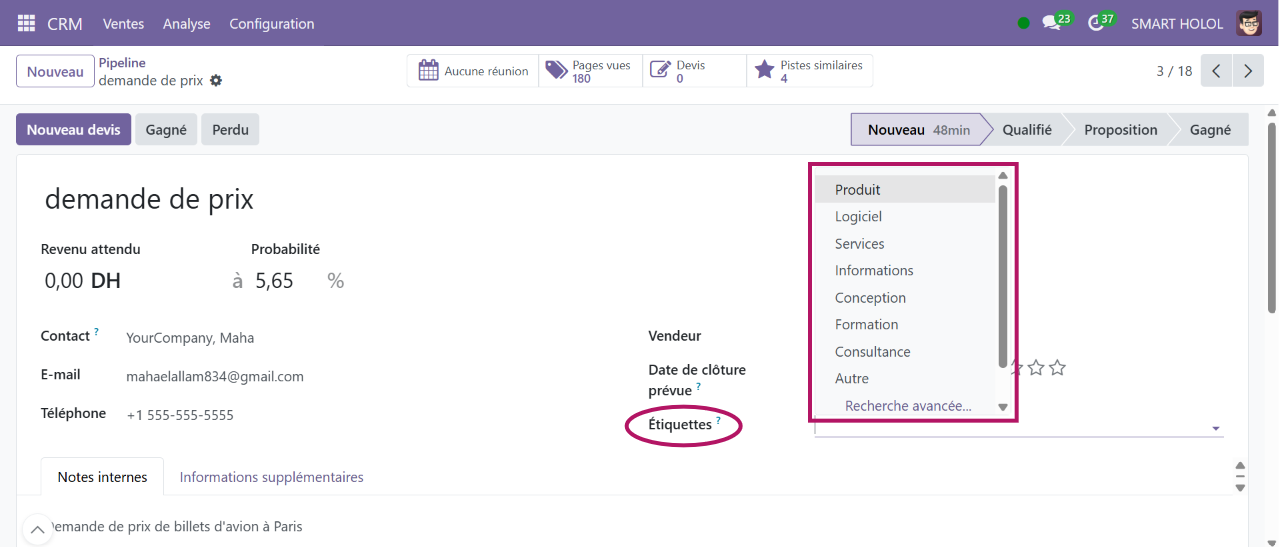
\includegraphics[width=\linewidth]{image/CRM/CRM17.png}
\caption{Qualification de l'opportunité à l'aide des étiquettes}
\label{fig:crm12_8}
\end{figure}
\section{PLANIFICATION D'ACTIVITÉS}

La gestion des relances commerciales (appels téléphoniques, rendez-vous, e-mails de suivi, etc.) est prise en charge nativement par le module \textbf{CRM} d'Odoo grâce aux \textbf{activités planifiées}. Ces activités permettent aux commerciaux de suivre leurs opportunités et de recevoir des rappels synchronisés avec leur calendrier.

Accéder au module \textbf{CRM}.

\begin{figure}[H]
\centering
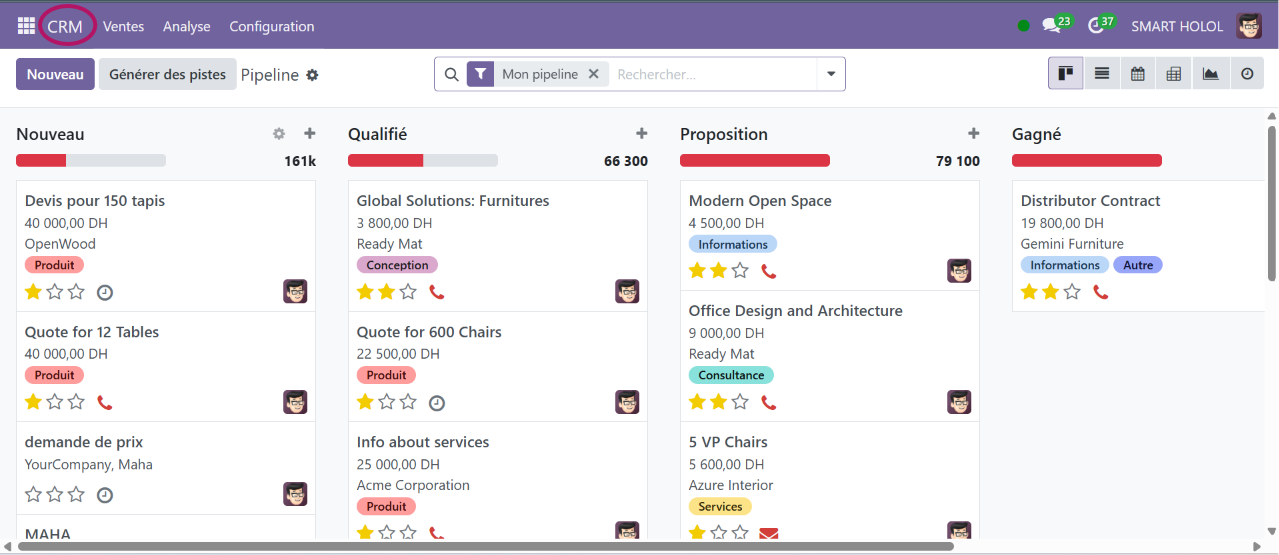
\includegraphics[width=\linewidth]{image/CRM/CRM10.png}
\caption{Accès au module CRM}
\label{fig:activite1}
\end{figure}

Sélectionner l'opportunité concernée dans le pipeline CRM.

\begin{figure}[H]
\centering
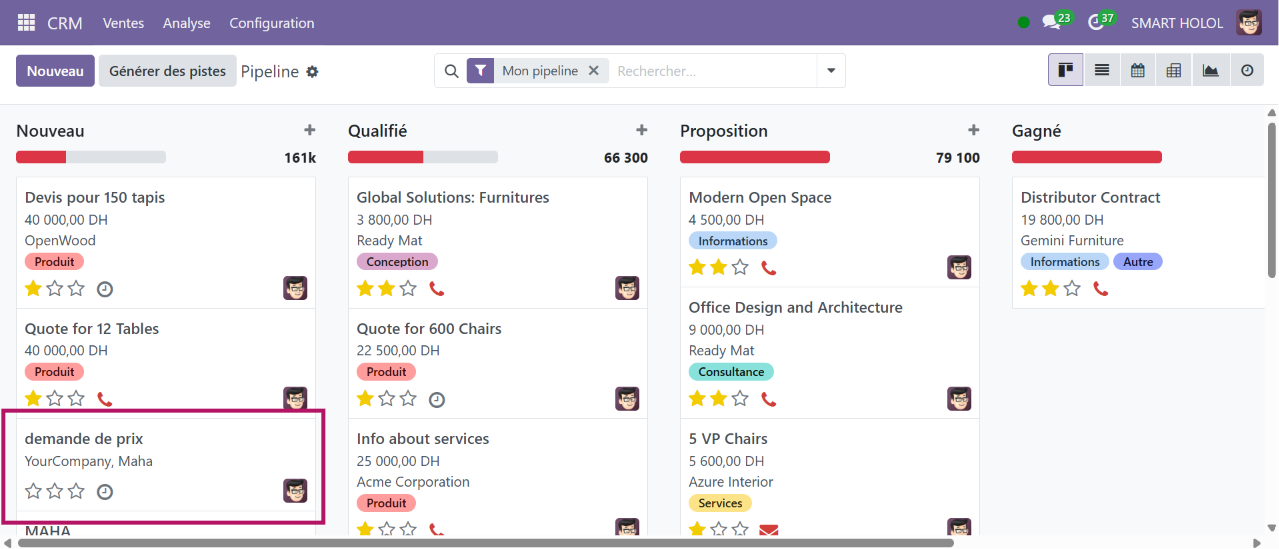
\includegraphics[width=\linewidth]{image/CRM/CRM18.png}
\caption{Sélection d'une opportunité}
\label{fig:activite2}
\end{figure}

Cliquer sur l'icône représentant une horloge afin de planifier une nouvelle activité.

\begin{figure}[H]
\centering
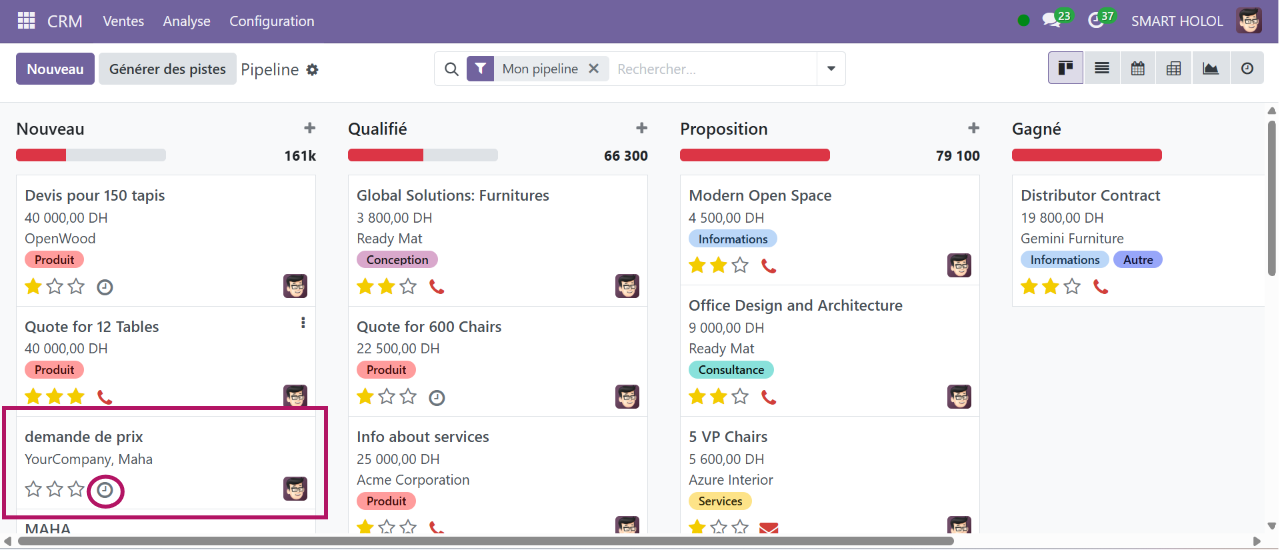
\includegraphics[width=\linewidth]{image/CRM/CRM19.png}
\caption{Accès à la planification des activités}
\label{fig:activite3}
\end{figure}

Choisir le type d'activité à planifier (appel, e-mail, réunion, tâche, etc.).

\begin{figure}[H]
\centering
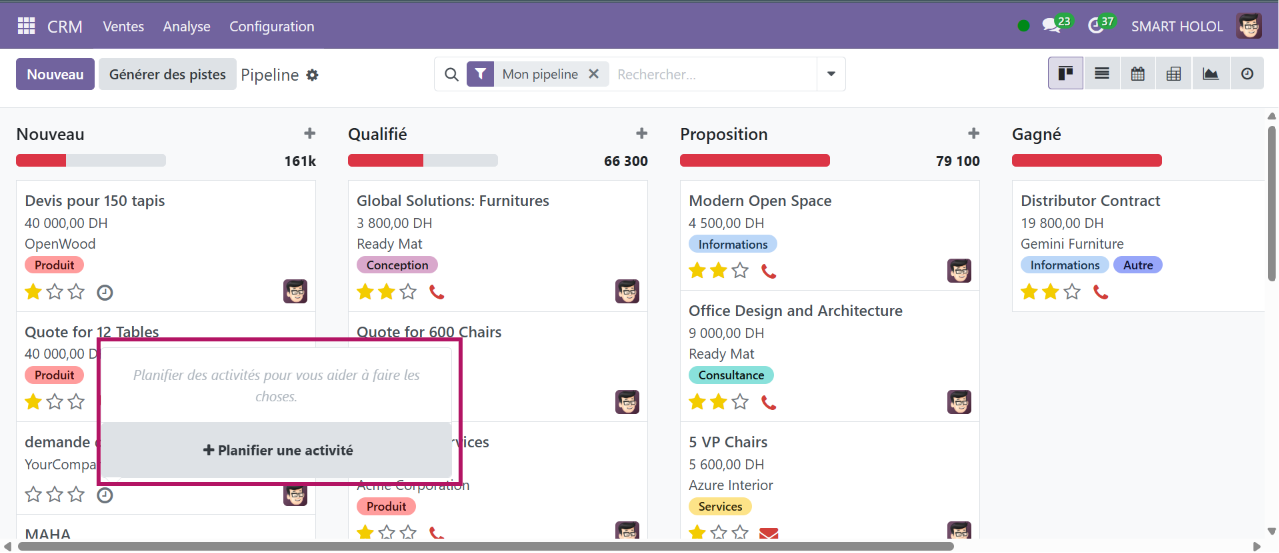
\includegraphics[width=\linewidth]{image/CRM/CRM20.png}
\caption{Planification d'une activité}
\label{fig:activite4}
\end{figure}

Renseigner les informations nécessaires, notamment le type d'activité, la date d'échéance, le responsable ainsi que les éventuelles notes, puis enregistrer.

\begin{figure}[H]
\centering
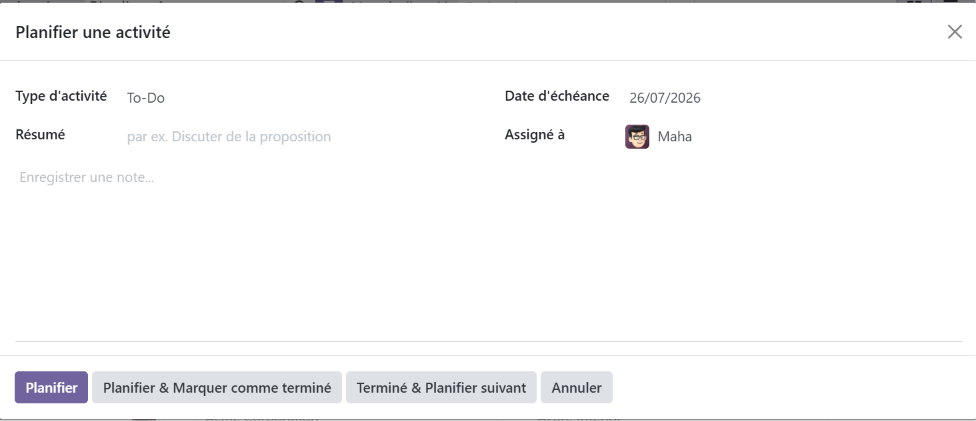
\includegraphics[width=\linewidth]{image/CRM/CRM21.png}
\caption{Configuration de l'activité planifiée}
\label{fig:activite5}
\end{figure}

Le statut des activités est indiqué par un code couleur permettant d'identifier rapidement leur état :

\begin{itemize}
    \item \textbf{Vert} : activité planifiée pour une date future ;
    \item \textbf{Orange} : activité prévue pour la journée en cours ;
    \item \textbf{Rouge} : activité en retard nécessitant une action immédiate.
\end{itemize}

Ce système facilite le suivi des relances clients et aide les commerciaux à respecter les échéances de leurs activités.

\section{REPORTING COMMERCIAL}

Le module \textbf{CRM} d'Odoo intègre des tableaux de bord d'analyse permettant de suivre les performances commerciales. Ces outils offrent une vision détaillée des opportunités, du taux de conversion par commercial, des performances des équipes ainsi que de la répartition des ventes selon différents critères. Les données peuvent être filtrées et regroupées dynamiquement afin de produire des analyses adaptées aux besoins de l'entreprise.

Accéder au module \textbf{CRM}.

\begin{figure}[H]
\centering
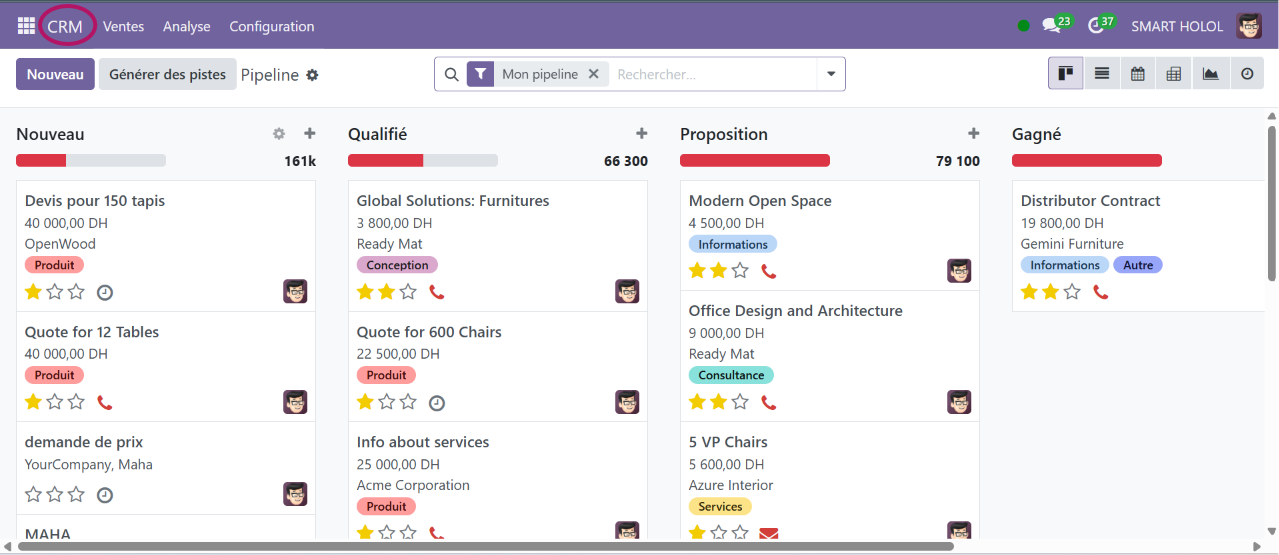
\includegraphics[width=\linewidth]{image/CRM/CRM10.png}
\caption{Accès au module CRM}
\label{fig:reporting1}
\end{figure}

Dans la barre de menus, sélectionner le menu \textbf{Analyse}.

\begin{figure}[H]
\centering
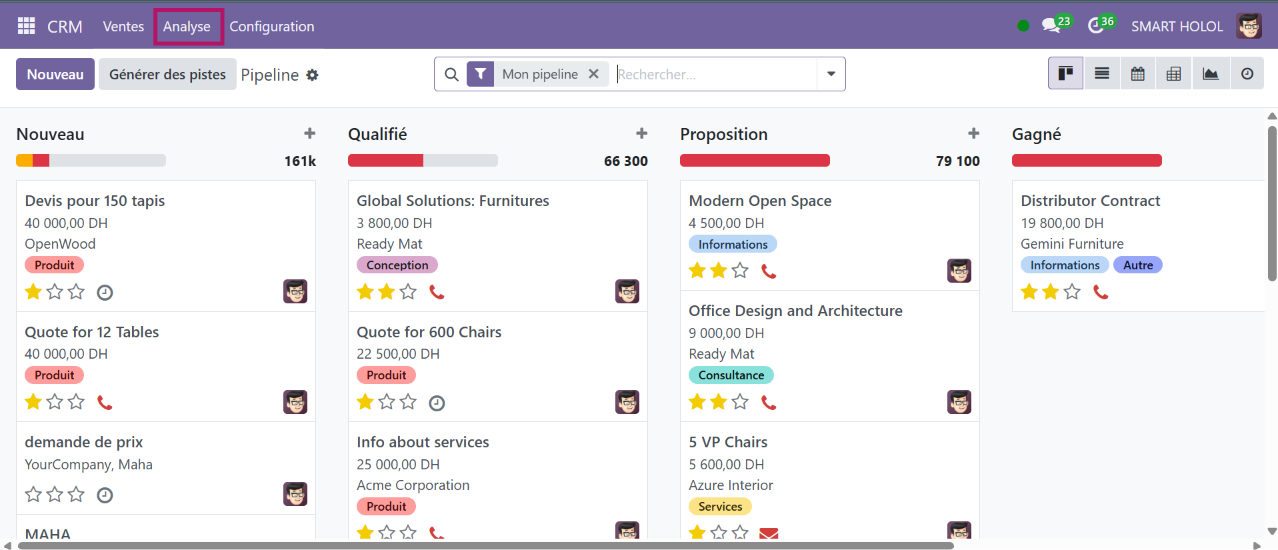
\includegraphics[width=\linewidth]{image/CRM/CRM22.png}
\caption{Accès aux analyses CRM}
\label{fig:reporting2}
\end{figure}

Choisir ensuite l'analyse du \textbf{Pipeline} afin de visualiser les statistiques relatives aux opportunités commerciales.

\begin{figure}[H]
\centering
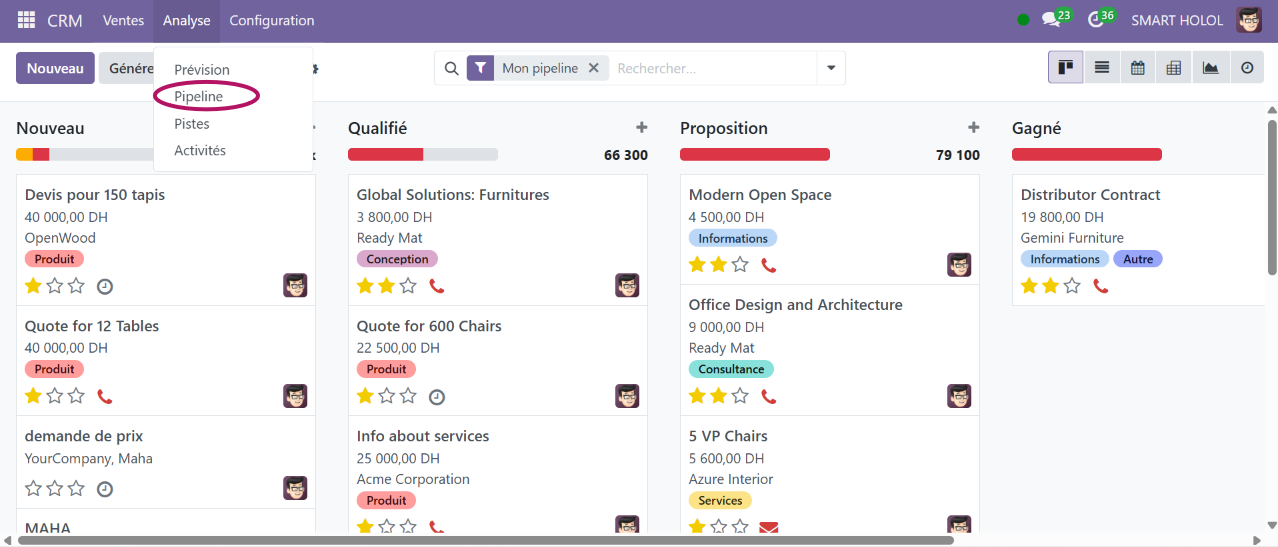
\includegraphics[width=\linewidth]{image/CRM/CRM23.png}
\caption{Analyse du pipeline commercial}
\label{fig:reporting3}
\end{figure}

Cliquer sur la barre de recherche pour accéder aux options de recherche, de filtrage et de regroupement.

\begin{figure}[H]
\centering
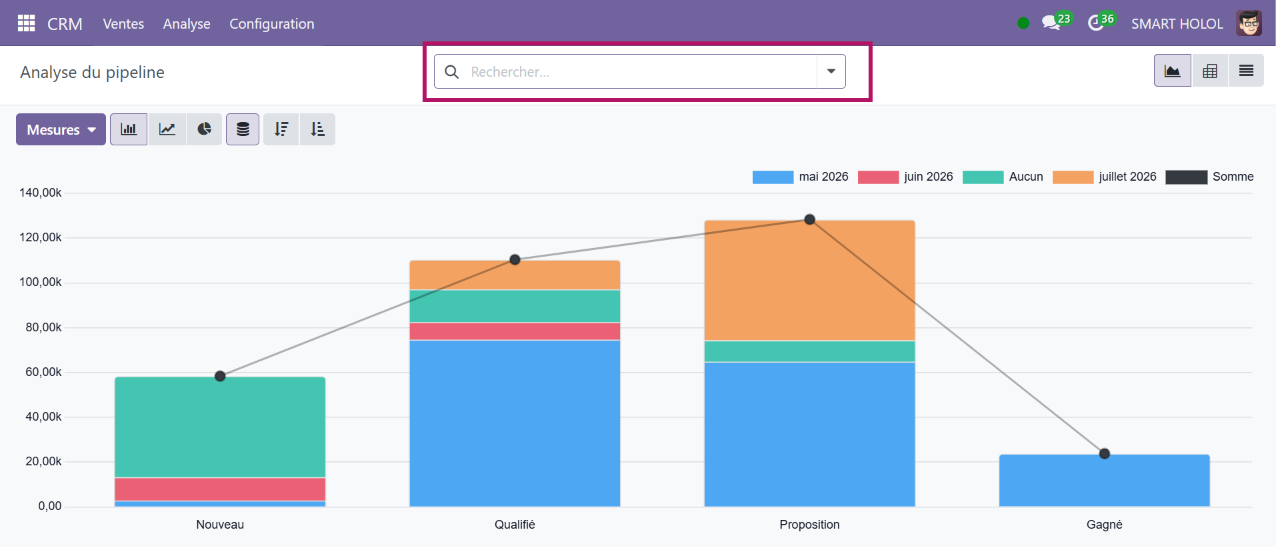
\includegraphics[width=\linewidth]{image/CRM/CRM24.png}
\caption{Accès aux options de recherche}
\label{fig:reporting4}
\end{figure}

Utiliser les options \textbf{Filtres} et \textbf{Regrouper par} pour analyser les données selon différents critères, tels que le commercial, l'équipe de vente, l'étape du pipeline, la date de création ou encore les étiquettes associées aux opportunités.

\begin{figure}[H]
\centering
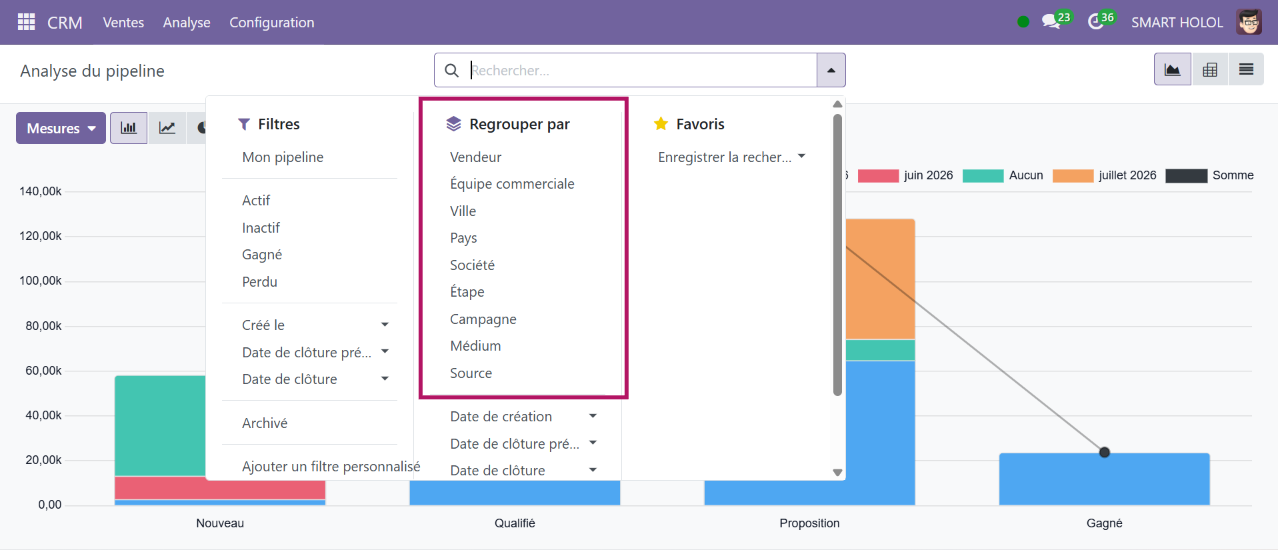
\includegraphics[width=\linewidth]{image/CRM/CRM25.png}
\caption{Filtrage et regroupement des données}
\label{fig:reporting5}
\end{figure}

Les tableaux de bord générés permettent de suivre les performances commerciales, notamment le nombre d'opportunités par vendeur, leur évolution dans le pipeline et le taux de conversion. Ils constituent un outil d'aide à la décision pour évaluer l'efficacité des actions commerciales et orienter les stratégies de prospection.

%=================================================
% MODULE VENTE
%=================================================
\chapter{Module VENTE}
\section{CRÉATION DE DEVIS}

La génération de devis détaillés permet de regrouper plusieurs prestations de voyage, telles que les vols, les transferts, l'hébergement et les excursions organisées, dans un document unique et structuré. Le module \textbf{Ventes} d'Odoo permet de créer des devis personnalisés en utilisant des sections et des sous-sections afin d'obtenir une présentation claire et attractive pour le client. Les devis peuvent ensuite être envoyés sous forme de document PDF ou consultés via une interface web.

Pour créer un devis, accédez tout d'abord au module \textbf{Ventes}.

\begin{figure}[H]
\centering
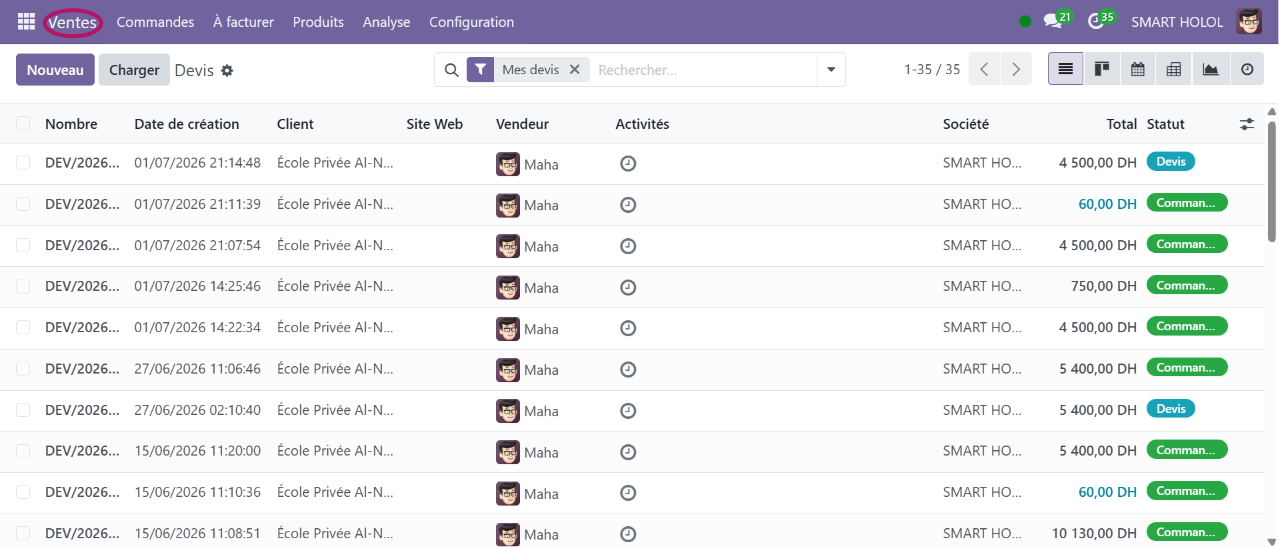
\includegraphics[width=\linewidth]{image/Ventes/vente17.png}
\caption{Accès au module Ventes}
\label{fig:vente_module}
\end{figure}


Depuis le menu \textbf{Commandes}, sélectionnez l'option \textbf{Devis}.

\begin{figure}[H]
\centering
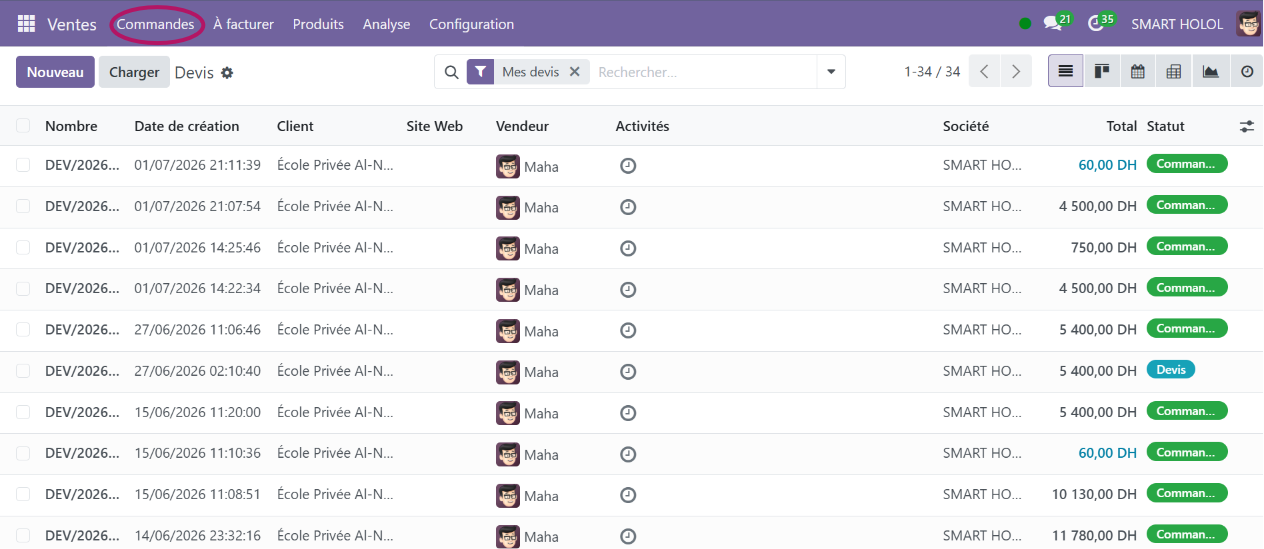
\includegraphics[width=\linewidth]{image/Ventes/vente7.png}
\caption{Accès au menu des commandes}
\label{fig:menu_commandes}
\end{figure}

\begin{figure}[H]
\centering
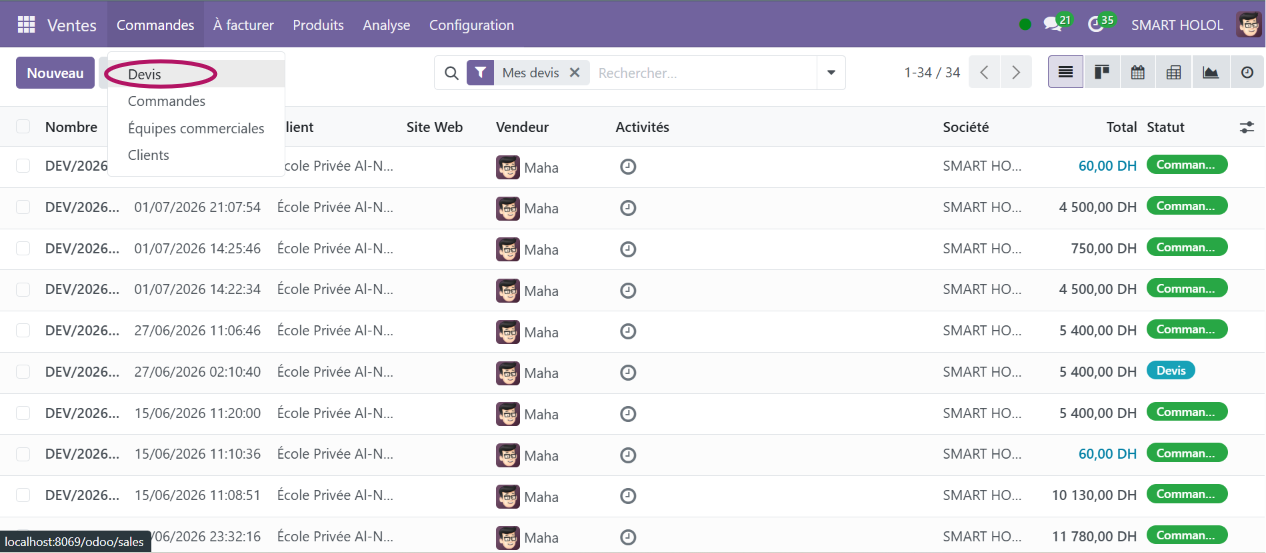
\includegraphics[width=\linewidth]{image/Ventes/vente8.png}
\caption{Liste des devis}
\label{fig:liste_devis}
\end{figure}


Cliquez ensuite sur \textbf{Nouveau} afin de créer un devis.

\begin{figure}[H]
\centering
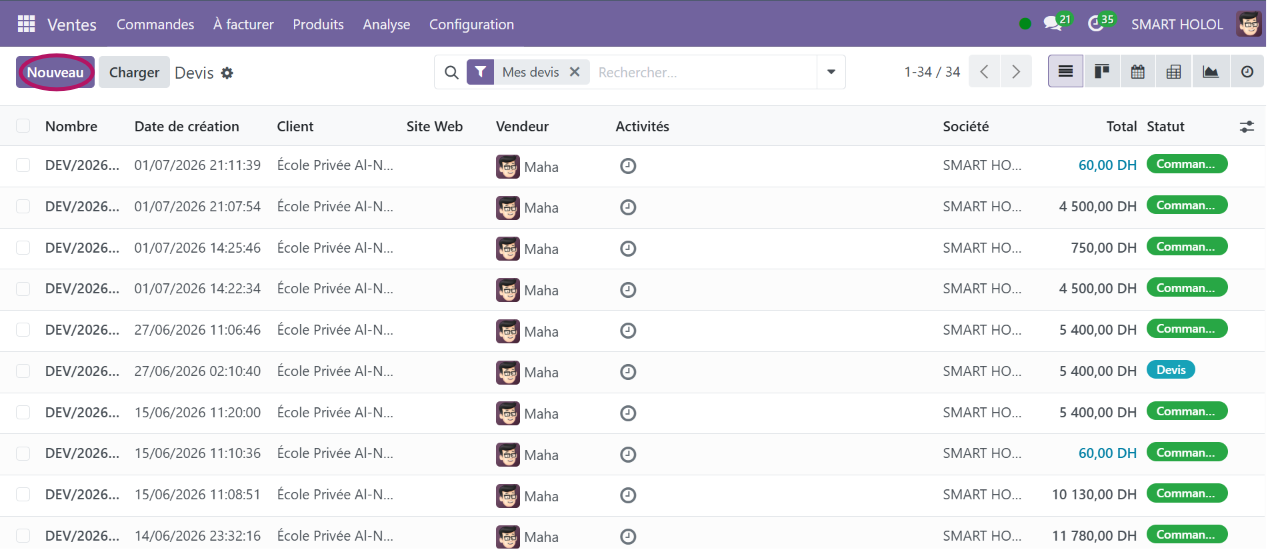
\includegraphics[width=\linewidth]{image/Ventes/vente9.png}
\caption{Création d'un nouveau devis}
\label{fig:nouveau_devis}
\end{figure}


Renseignez les informations nécessaires, notamment le client, la date d'Expiration ainsi que les autres informations générales du devis.

\begin{figure}[H]
\centering
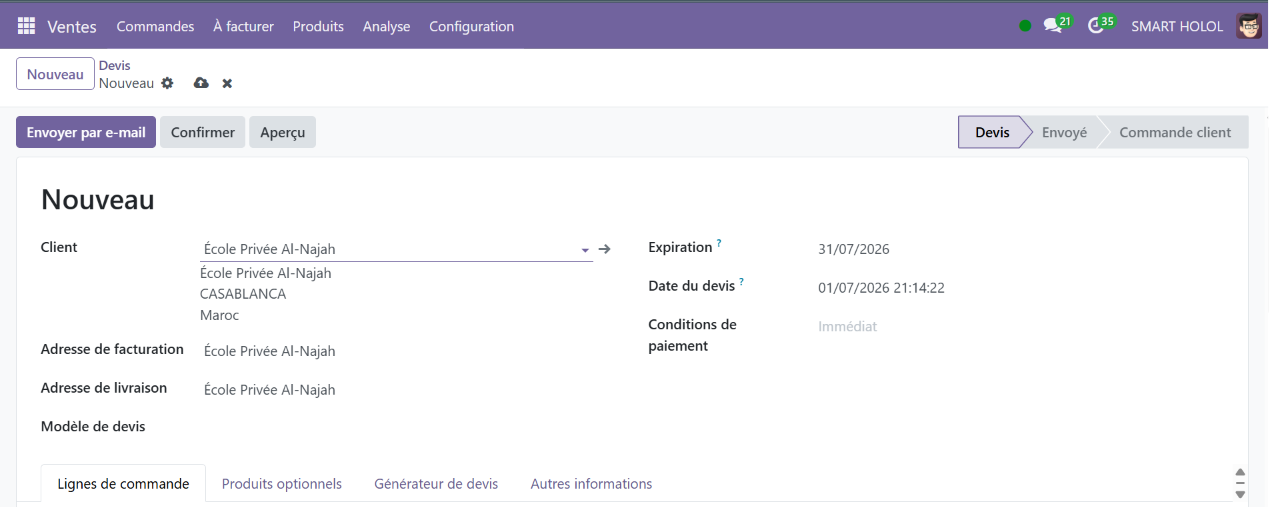
\includegraphics[width=\linewidth]{image/Ventes/vente10.png}
\caption{Saisie des informations du devis}
\label{fig:info_devis}
\end{figure}


Dans la section \textbf{Lignes de commande}, cliquez sur \textbf{Ajouter une section} avant d'ajouter les produits.

\begin{figure}[H]
\centering
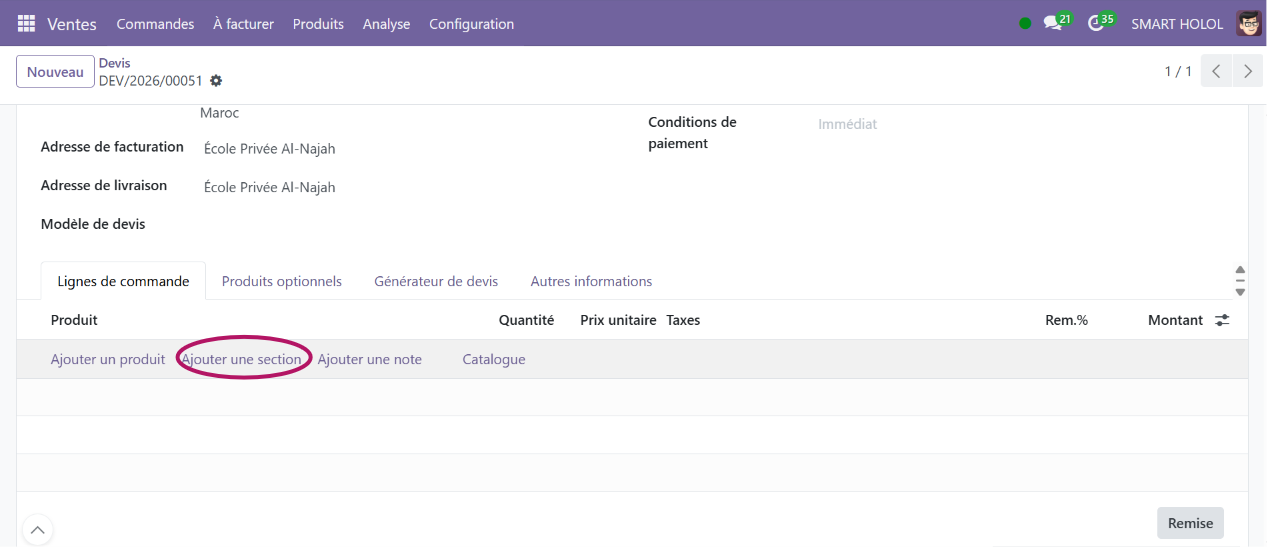
\includegraphics[width=\linewidth]{image/Ventes/vente11.png}
\caption{Ajout d'une section au devis}
\label{fig:ajout_section}
\end{figure}

Saisissez ensuite le titre de la section correspondant à la catégorie de prestations (par exemple : Transport, Hôtel, Excursion ou Transfert).

\begin{figure}[H]
\centering
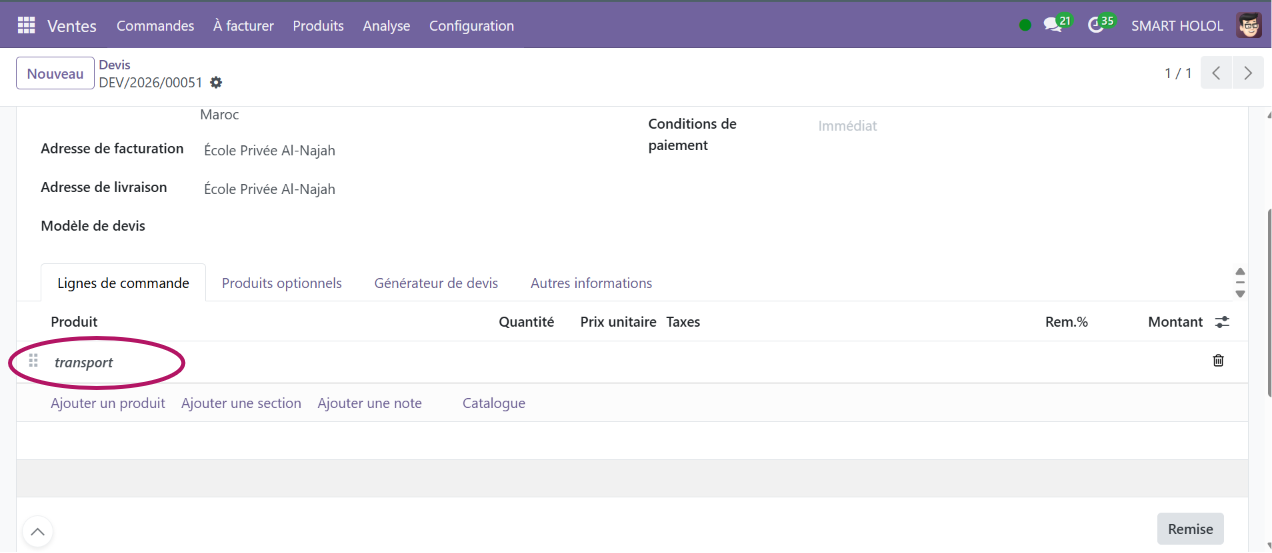
\includegraphics[width=\linewidth]{image/Ventes/vente12.png}
\caption{Définition du titre de la section}
\label{fig:titre_section}
\end{figure}


Cliquez sur \textbf{Ajouter un produit} afin d'insérer les prestations dans la section créée.

\begin{figure}[H]
\centering
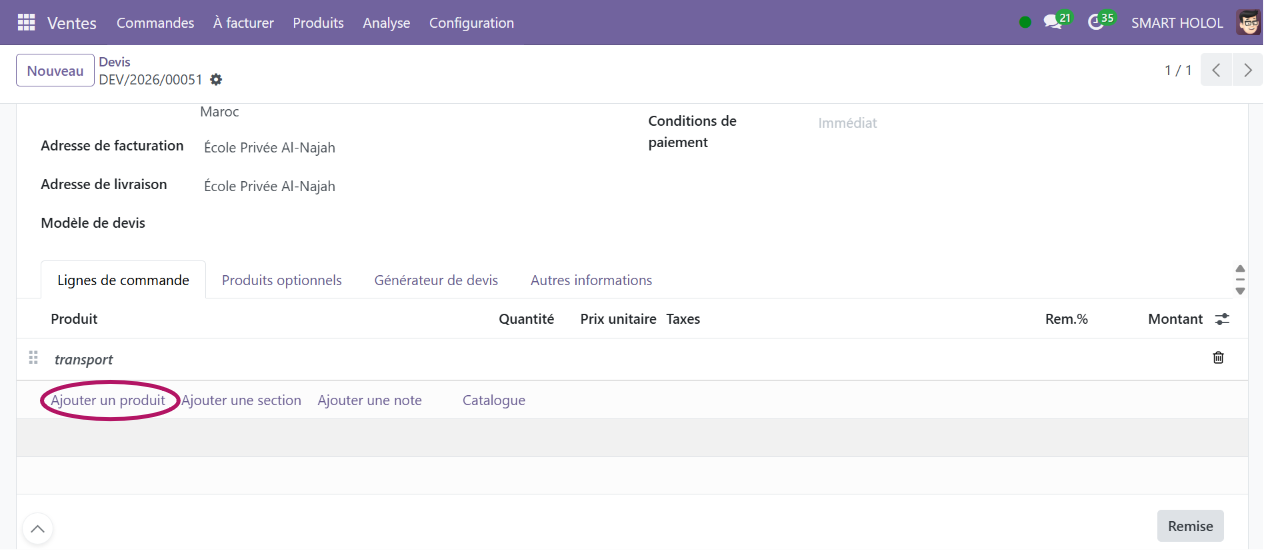
\includegraphics[width=\linewidth]{image/Ventes/vente13.png}
\caption{Ajout d'un produit au devis}
\label{fig:ajout_produit}
\end{figure}

Sélectionnez les produits correspondant à chaque section du devis.

\begin{figure}[H]
\centering
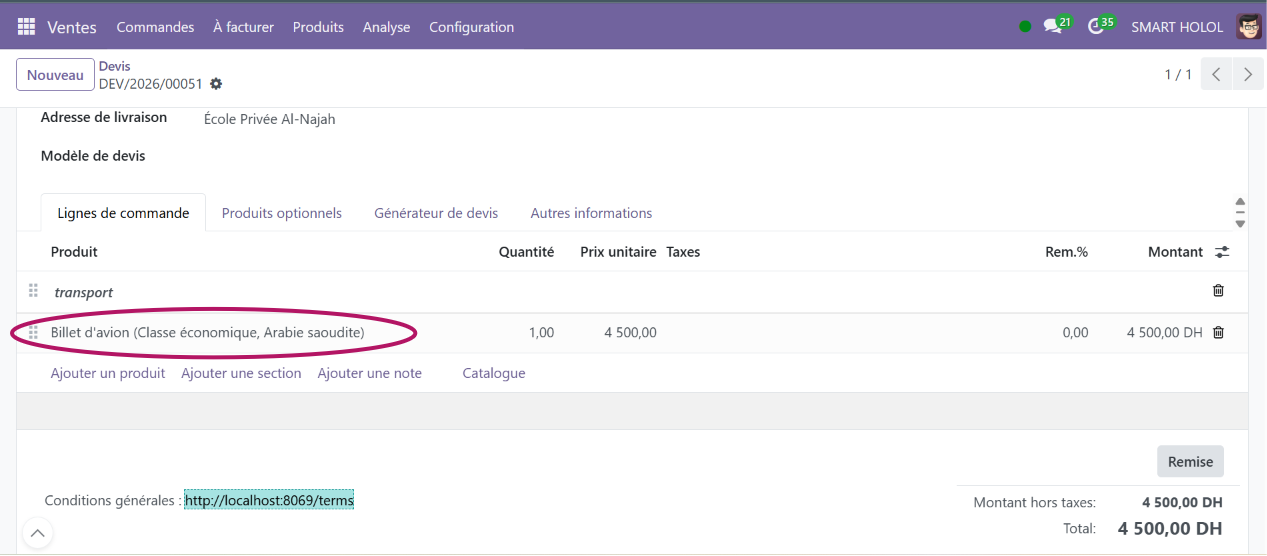
\includegraphics[width=\linewidth]{image/Ventes/vente14.png}
\caption{Sélection des produits par section}
\label{fig:selection_produits}
\end{figure}

Une fois le devis complété, cliquez sur \textbf{Aperçu} pour visualiser le rendu final du devis avant son envoi au client.


\begin{figure}[H]
\centering
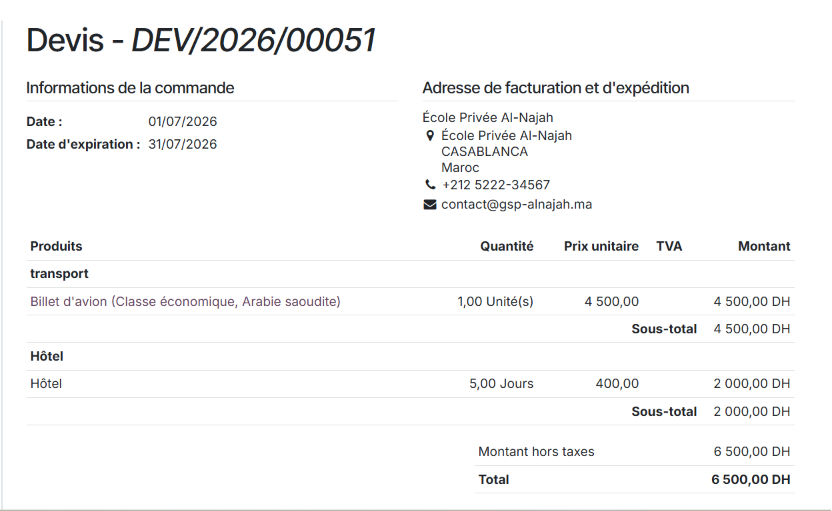
\includegraphics[width=\linewidth]{image/Ventes/vente16.png}
\caption{Aperçu du devis}
\label{fig:apercu_devis}
\end{figure}

Enfin, cliquez sur \textbf{Confirmer} afin de l'enregistrer.

\begin{figure}[H]
\centering
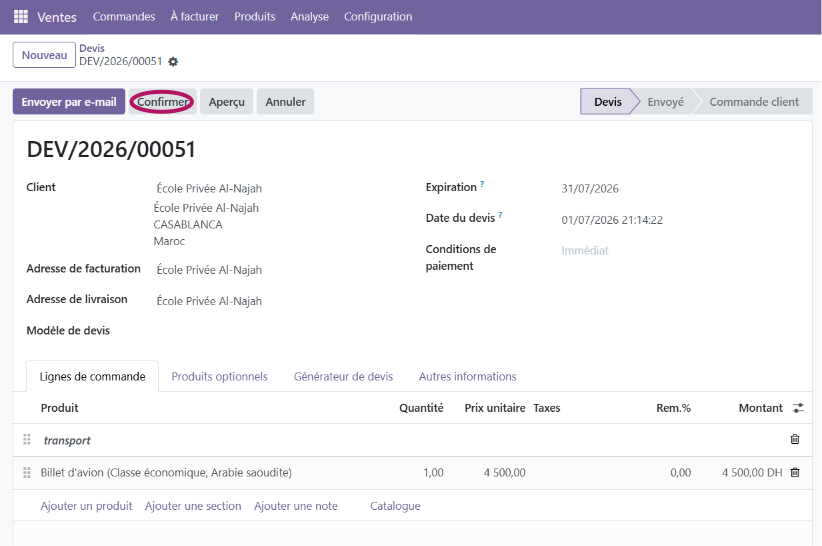
\includegraphics[width=\linewidth]{image/Ventes/vente15.png}
\caption{Confirmation du devis}
\label{fig:confirmation_devis}
\end{figure}



\section{RÈGLEMENTS \& FACTURES D'ACOMPTES}

La gestion des acomptes permet de mettre en place une facturation progressive, par exemple en demandant un acompte de 30\% lors de la réservation, puis le règlement du solde avant le départ. Cette fonctionnalité est prise en charge nativement par le module \textbf{Ventes} d'Odoo, qui permet de créer des factures d'acomptes sous forme de pourcentage ou de montant fixe.

Pour créer une facture d'acompte, accédez tout d'abord au module \textbf{Ventes}.

\begin{figure}[H]
\centering
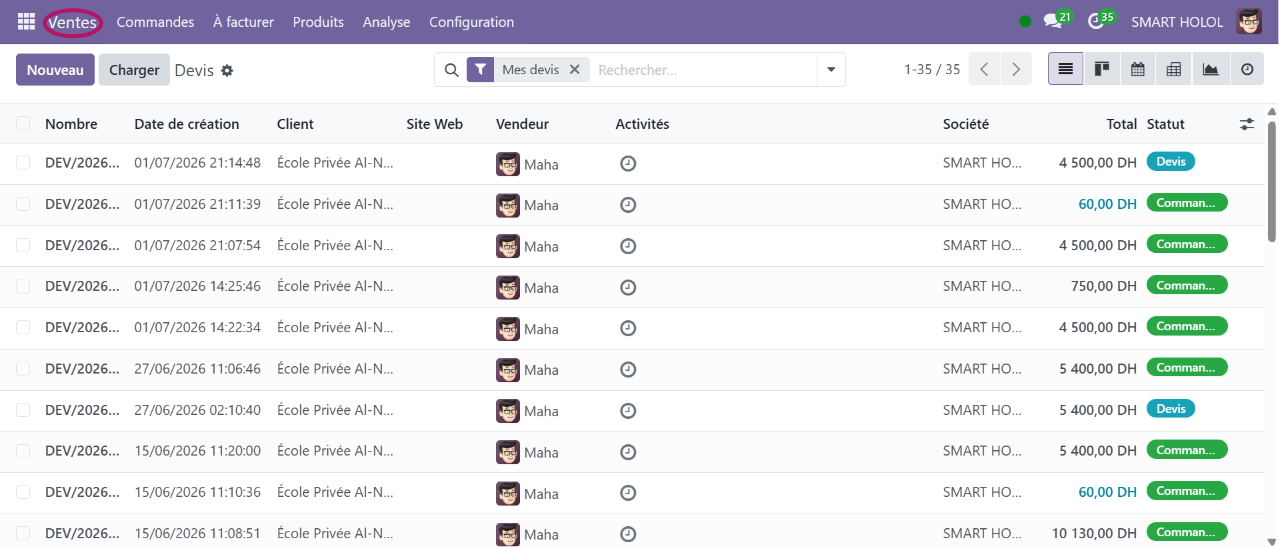
\includegraphics[width=\linewidth]{image/Ventes/vente17.png}
\caption{Accès au module Ventes}
\label{fig:vente_module_acompte}
\end{figure}

Depuis le menu \textbf{À facturer}, sélectionnez \textbf{Commandes à facturer}.

\begin{figure}[H]
\centering
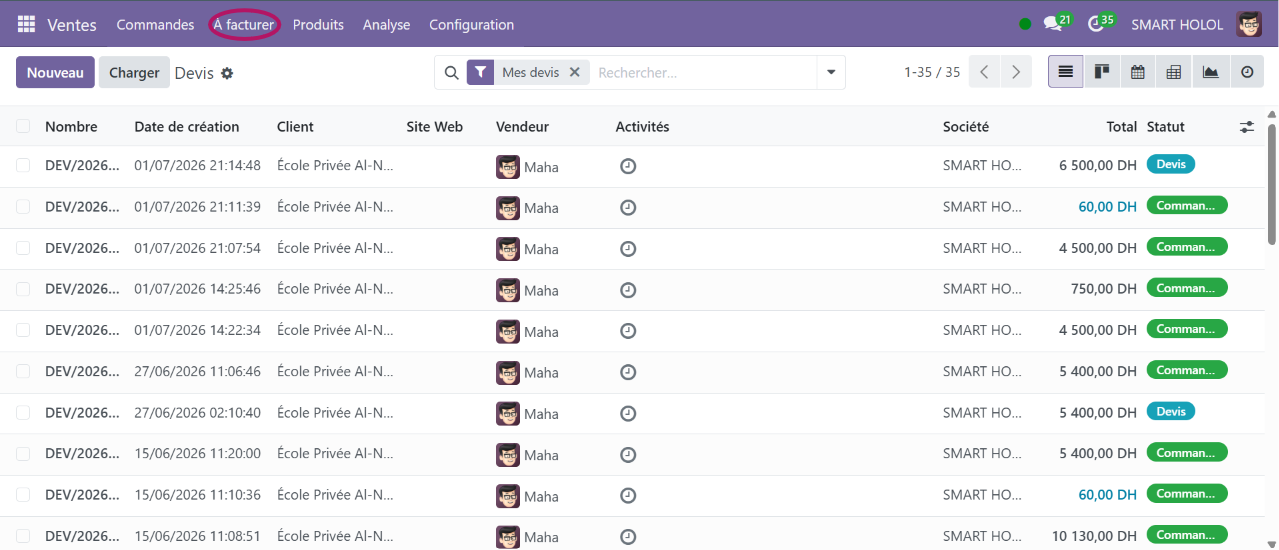
\includegraphics[width=\linewidth]{image/Ventes/vente18.png}
\caption{Accès au menu À facturer}
\label{fig:menu_a_facturer}
\end{figure}

\begin{figure}[H]
\centering
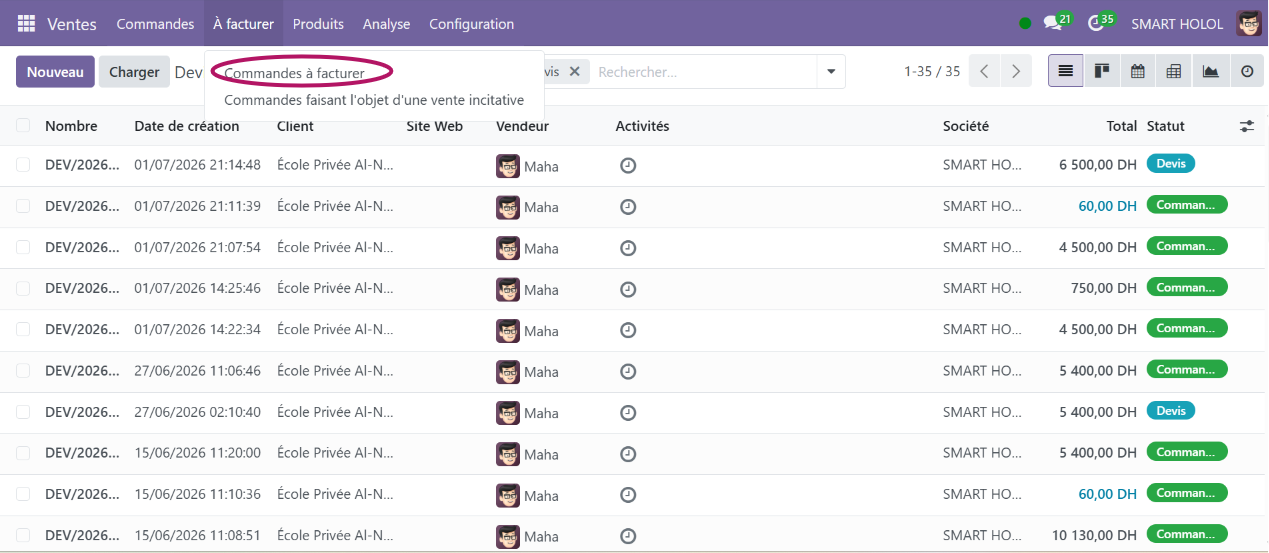
\includegraphics[width=\linewidth]{image/Ventes/vente19.png}
\caption{Liste des commandes à facturer}
\label{fig:commandes_a_facturer}
\end{figure}

Sélectionnez ensuite la commande concernée dans la liste.

\begin{figure}[H]
\centering
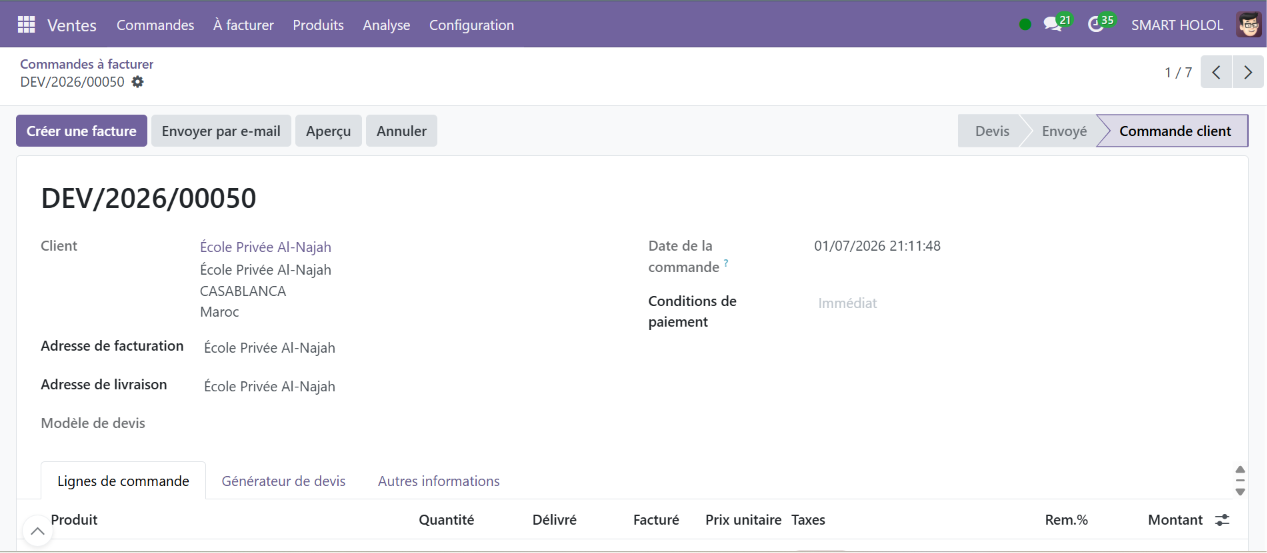
\includegraphics[width=\linewidth]{image/Ventes/vente20.png}
\caption{Sélection d'une commande}
\label{fig:selection_commande}
\end{figure}


Cliquez sur \textbf{Créer une facture}.

\begin{figure}[H]
\centering
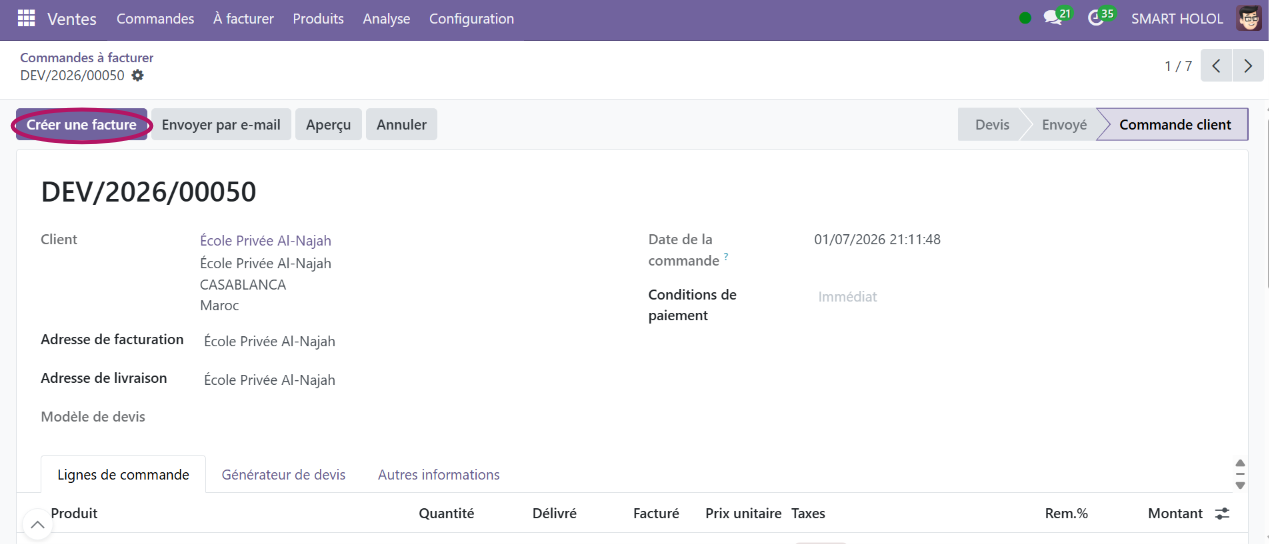
\includegraphics[width=\linewidth]{image/Ventes/vente21.png}
\caption{Création d'une facture}
\label{fig:creation_facture}
\end{figure}

Choisissez le type d'acompte souhaité : \textbf{Acompte (pourcentage)} ou \textbf{Acompte (montant fixe)}, puis renseignez la valeur correspondante.

\begin{figure}[H]
\centering
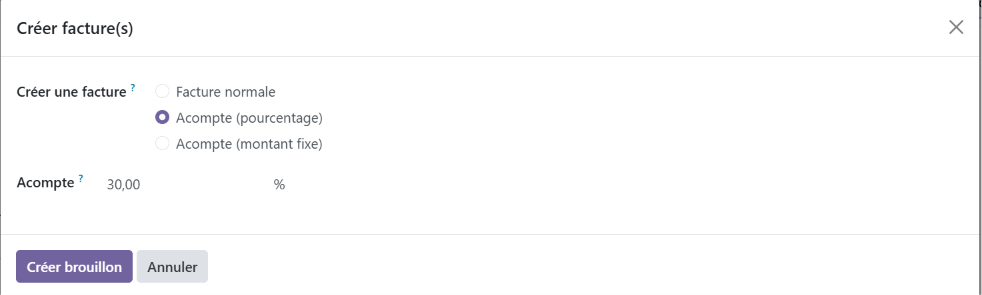
\includegraphics[width=\linewidth]{image/Ventes/vente22.png}
\caption{Configuration de l'acompte}
\label{fig:configuration_acompte}
\end{figure}

Cliquez ensuite sur \textbf{Créer un brouillon} afin de générer la facture d'acompte.

\begin{figure}[H]
\centering
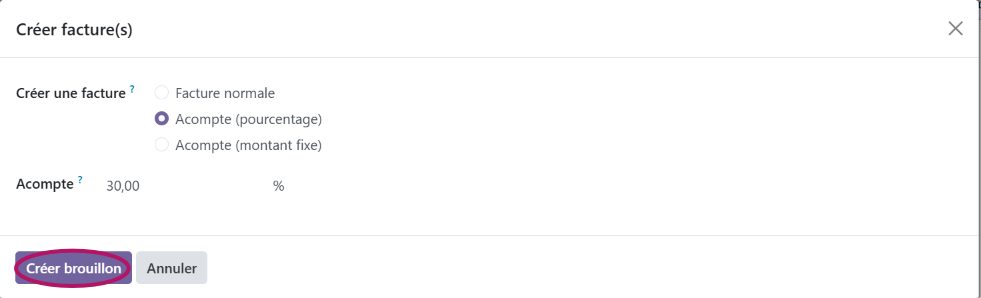
\includegraphics[width=\linewidth]{image/Ventes/vente23.png}
\caption{Création du brouillon de facture}
\label{fig:brouillon_facture}
\end{figure}


Une fois la facture générée, cliquez sur \textbf{Confirmer} pour la valider.


\begin{figure}[H]
\centering
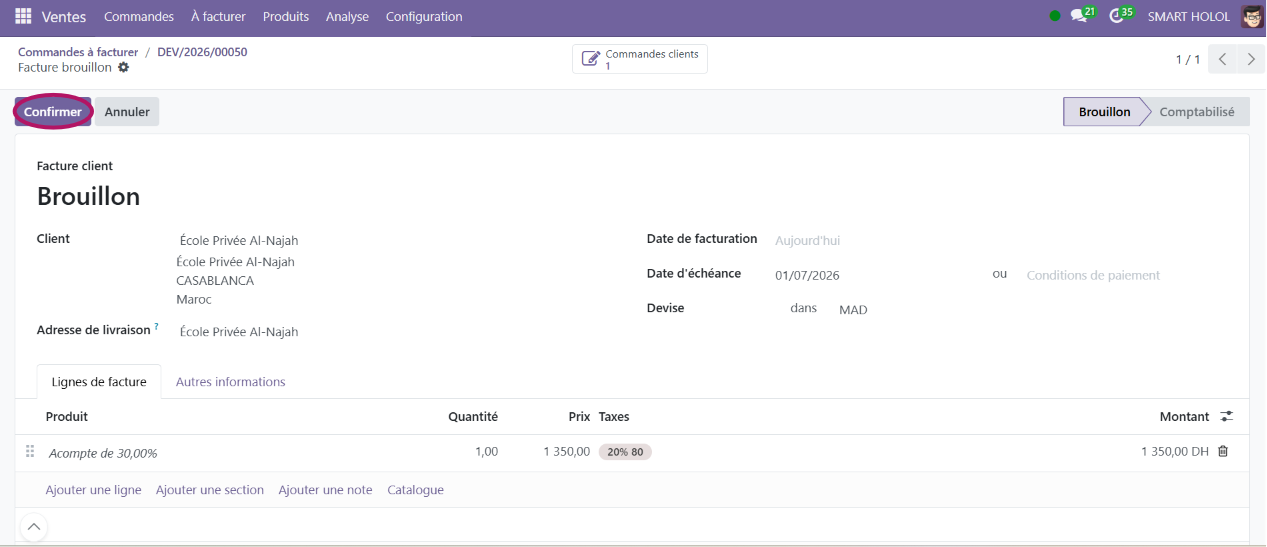
\includegraphics[width=\linewidth]{image/Ventes/vente24.png}
\caption{Validation de la facture}
\label{fig:validation_facture}
\end{figure}


Il est ensuite possible de cliquer sur \textbf{Aperçu} afin de visualiser la facture avant son impression ou son envoi au client.

\begin{figure}[H]
\centering
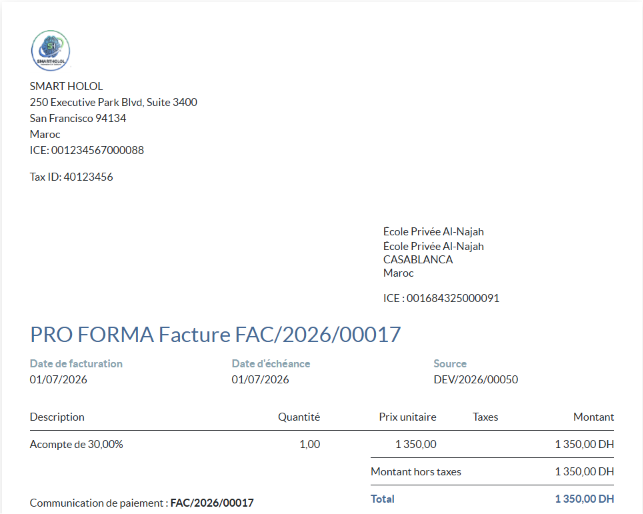
\includegraphics[width=\linewidth]{image/Ventes/vente25.png}
\caption{Aperçu de la facture d'acompte}
\label{fig:apercu_facture}
\end{figure}

Le bouton \textbf{Imprimer} permet de télécharger la facture au format PDF, tandis que le bouton \textbf{Payer} permet d'enregistrer un règlement en choisissant le montant à payer.

\begin{figure}[H]
\centering
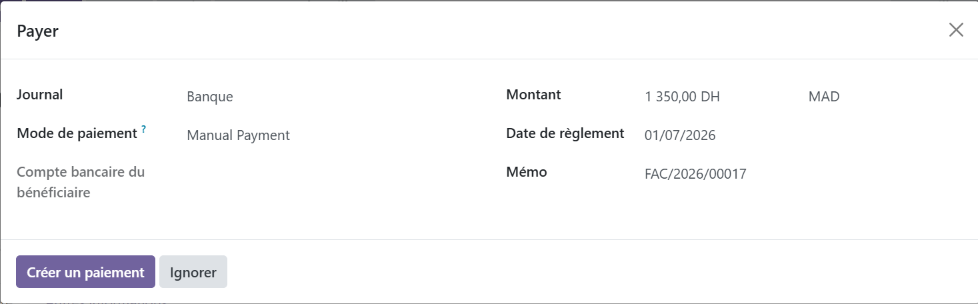
\includegraphics[width=\linewidth]{image/Ventes/vente26.png}
\caption{Enregistrement du paiement}
\label{fig:paiement_facture}
\end{figure}


Selon le montant saisi, la facture peut être enregistrée avec un \textbf{paiement partiel}.


\begin{figure}[H]
\centering
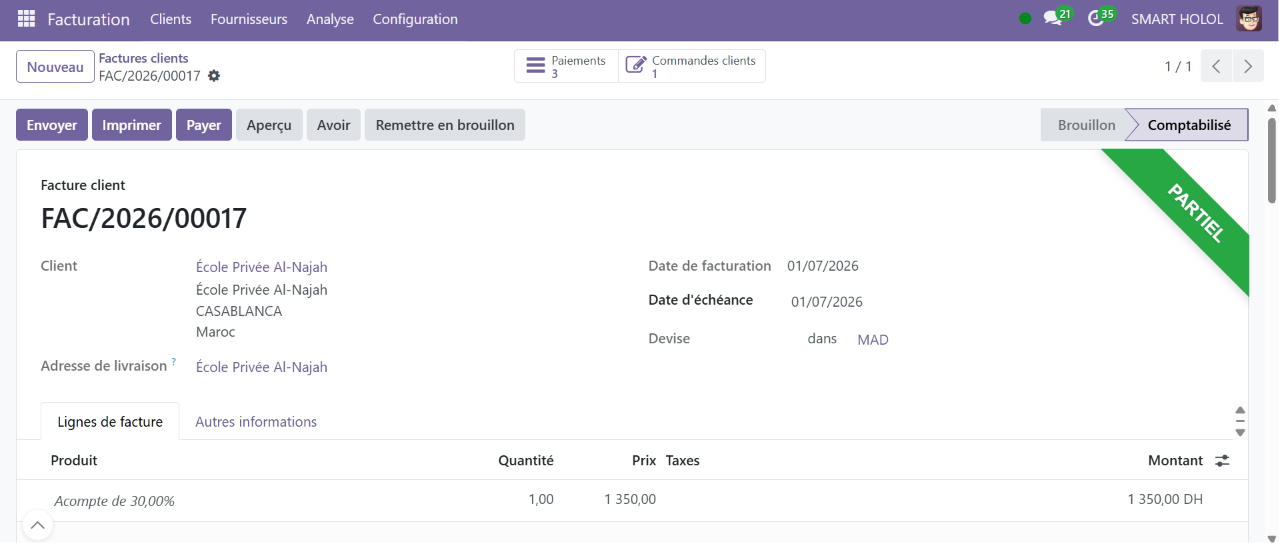
\includegraphics[width=\linewidth]{image/Ventes/vente28.png}
\caption{Exemple de paiement partiel}
\label{fig:paiement_partiel}
\end{figure}


Si le montant total de la facture est réglé, celle-ci est automatiquement marquée comme \textbf{entièrement payée}.

\begin{figure}[H]
\centering
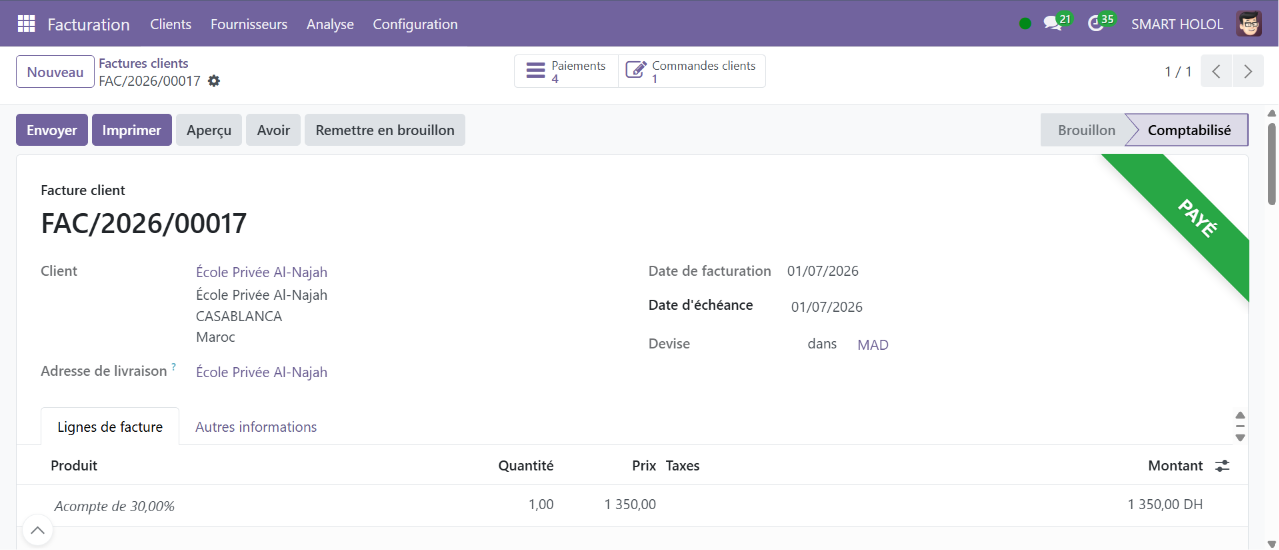
\includegraphics[width=\linewidth]{image/Ventes/vente29.png}
\caption{Exemple de paiement total}
\label{fig:paiement_total}
\end{figure}
```




%=================================================
% MODULE FACTURATION
%=================================================
\chapter{Module FACTURATION}
\section{FACTURATION CLIENTS}
\subsection{Création de factures adaptées au secteur avec TVA sur la marge bénéficiaire (Régime fiscal des agences de voyage).
}
Pour configurer les taxes de manière à ce qu'elles soient prises en compte lors du paiement sans être affichées sur la facture du client, il est nécessaire, lors de la création du produit, de saisir directement un prix incluant la taxe, la marge bénéficiaire ainsi que tous les autres coûts supplémentaires.

Accédez ensuite au module Facturation:

\begin{figure}[H]
\centering
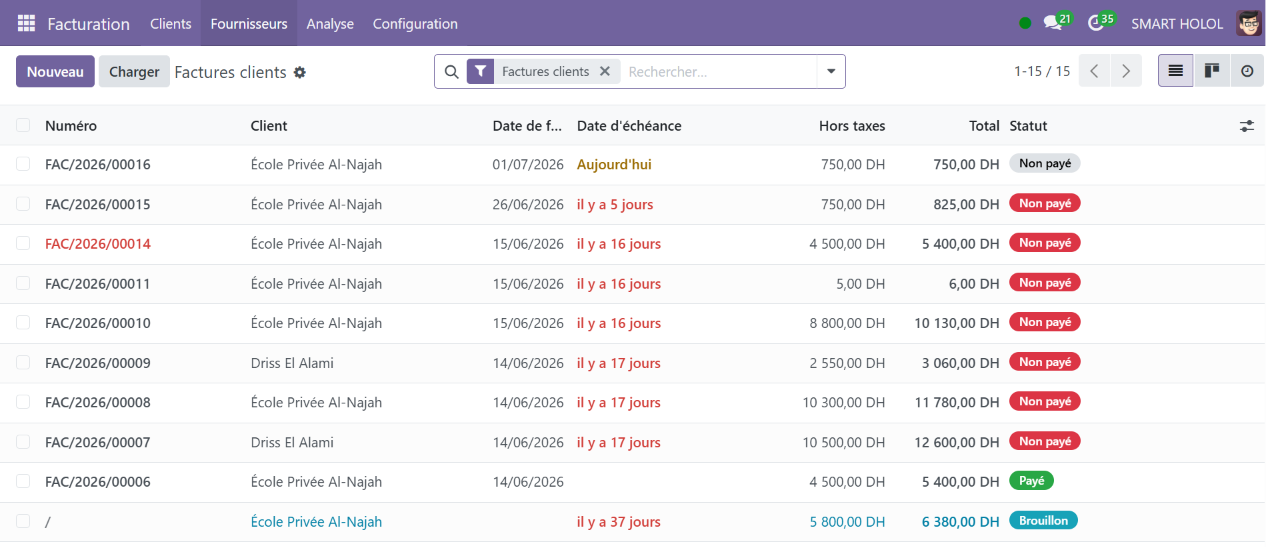
\includegraphics[width=\linewidth]{image/facturation/facturation0.png}
\caption{Liste des factures}
\label{fig:achat1}
\end{figure}


Il est possible de créer une nouvelle facture en accédant au menu :

\textbf{Facturation $\rightarrow$ Nouveau}.

\begin{figure}[H]
\centering
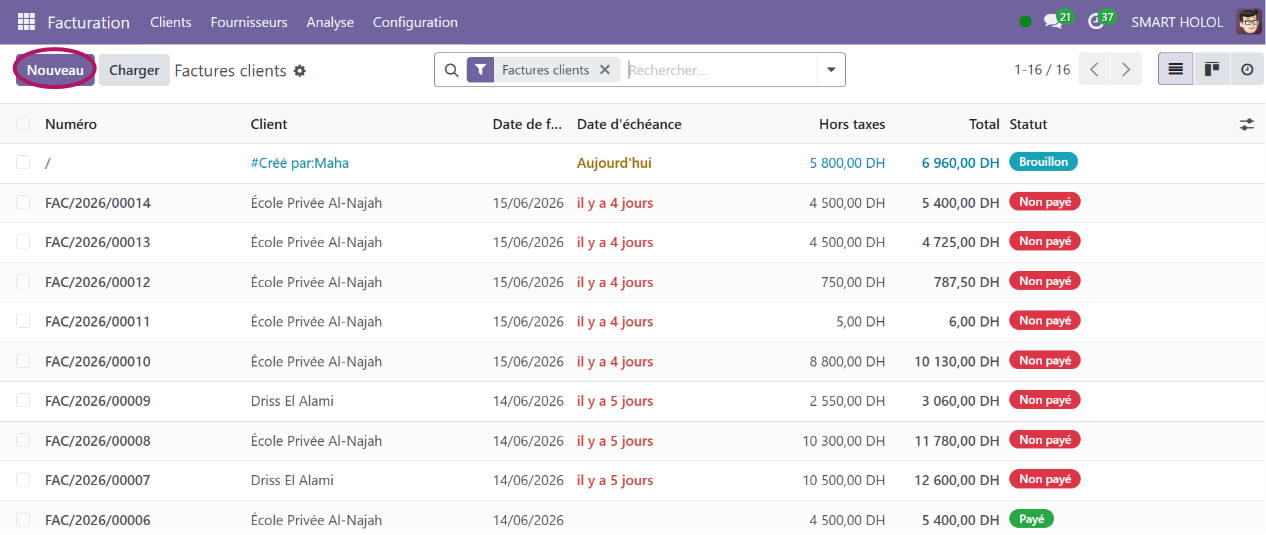
\includegraphics[width=\linewidth]{image/facturation/facturation 4.png}
\caption{Création d'une nouvelle facture}
\label{fig:new_invoice}
\end{figure}

Renseignez ensuite les informations nécessaires, telles que le client, la date de facturation, les produits ou services concernés, ainsi que les quantités et les montants associés.

Une fois les lignes de facture ajoutées, vérifiez si une TVA est associée au produit. Si c'est le cas, supprimez-la.

\begin{figure}[H]
\centering
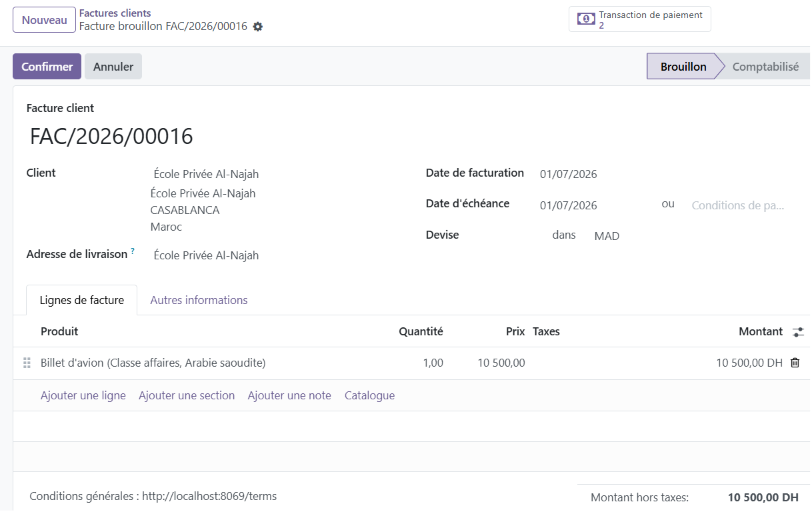
\includegraphics[width=\linewidth]{image/facturation/facturation6.png}
\caption{Suppression de la TVA associée au produit}
\label{fig:new_invoice}
\end{figure}

ensuite on click sur **confirmer**
\begin{figure}[H]
\centering
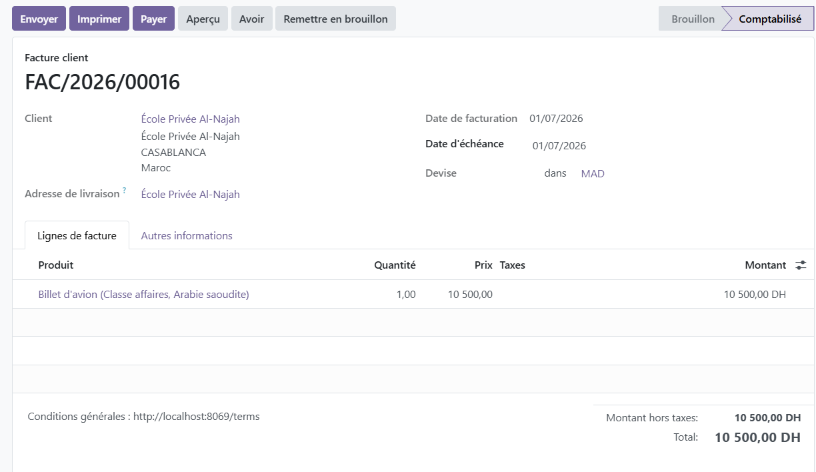
\includegraphics[width=\linewidth]{image/facturation/facturation7.png}
\caption{confirmation de la facture client}
\label{fig:new_invoice}
\end{figure}
Enfin, il est possible de sélectionner **Payer** pour enregistrer le paiement ou **Aperçu** afin de visualiser la facture avant sa validation.

\begin{figure}[H]
\centering
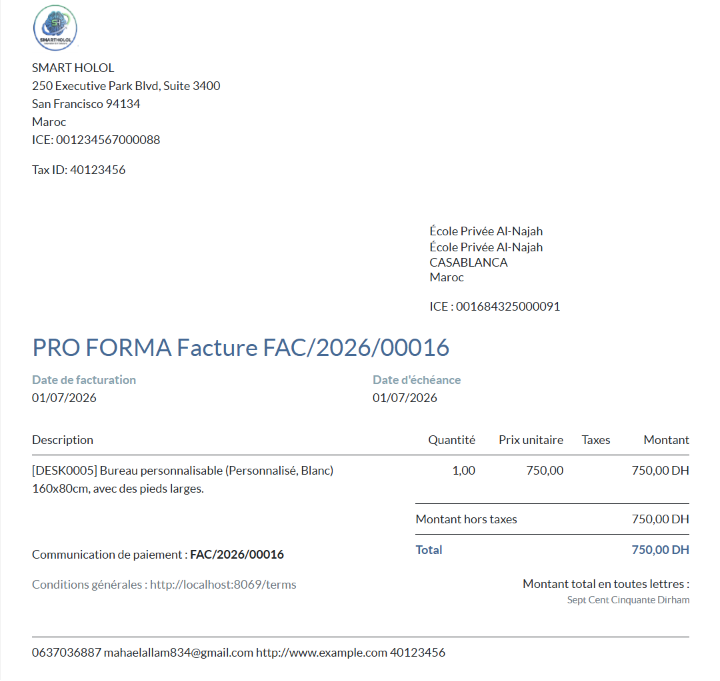
\includegraphics[width=\linewidth]{image/facturation/exemple_facture.png}
\caption{Aperçu de la facture}
\label{fig:new_invoice}
\end{figure}


%=================================================
% MODULE ACHAT
%=================================================
\chapter{Module ACHAT}
\section{GESTION DES PRESTATAIRES}

La centralisation de la base de données des hôtels, des compagnies de transport, des guides et des réceptifs partenaires, ainsi que la gestion des sous-traitants et des fournisseurs, sont assurées nativement par Odoo grâce aux modules \textbf{Contacts} et \textbf{Achats}.

Pour accéder à ces informations, il suffit d'ouvrir le module \textbf{Contact}, cette interface regroupe l'ensemble des contacts enregistrés dans le système, notamment les fournisseurs, les clients et les autres partenaires, permettant ainsi une gestion centralisée et un accès rapide à leurs informations.
\begin{figure}[H]
\centering
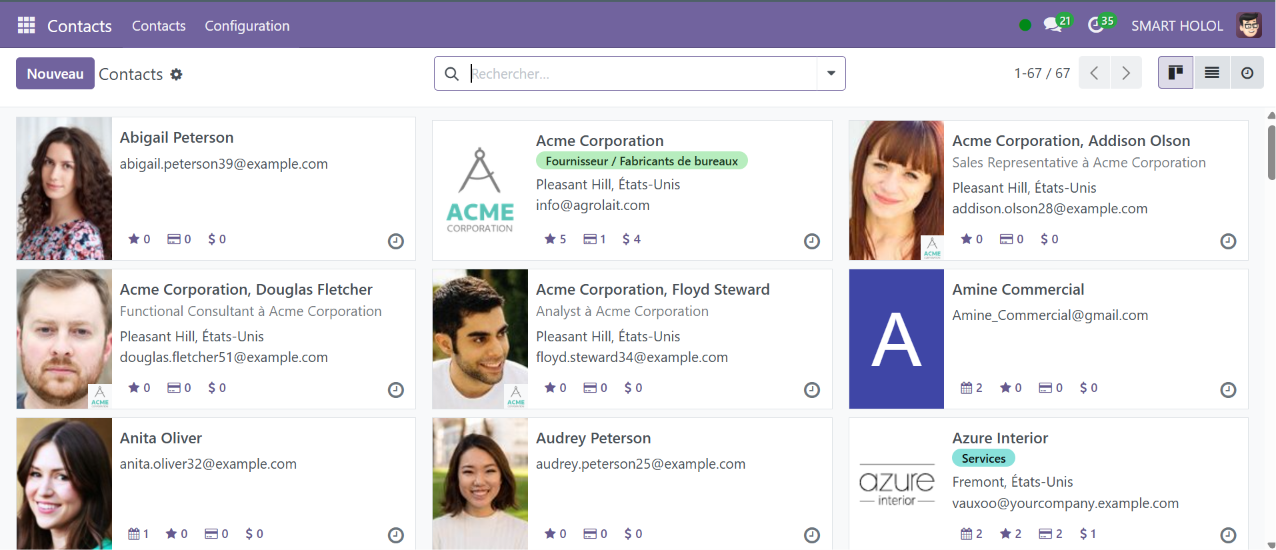
\includegraphics[width=\linewidth]{image/Achat/Contact.png}
\caption{Module Contacts}
\label{fig:invoice_tax}
\end{figure}

\section{COMMANDES DE PRESTATIONS}

L'émission et l'envoi des demandes de réservation ainsi que des bons de commande destinés aux hôtels, transporteurs et autres prestataires sont assurés par le module standard \textbf{Achats} d'Odoo.

Ce module permet de générer automatiquement des demandes de prix (utilisées comme demandes de réservation) et, après validation, de créer des bons de commande pouvant être envoyés au fournisseur au format PDF par courrier électronique.

Pour créer une demande de prix, accéder au module \textbf{Achats}, puis sélectionner le menu \textbf{Commandes > Demandes de prix}.

\begin{figure}[H]
\centering
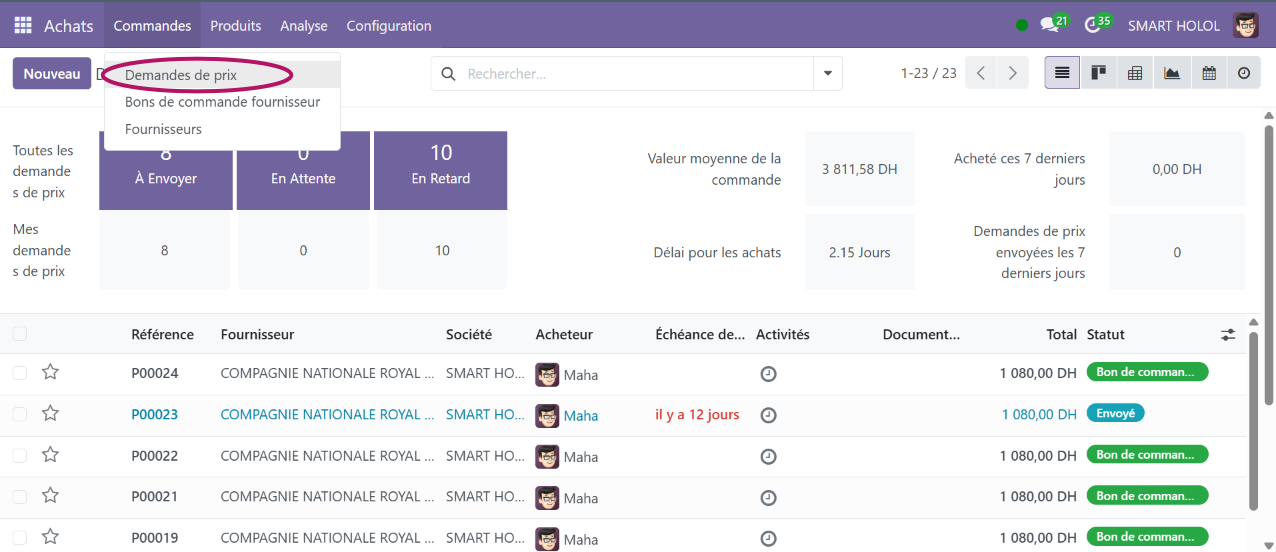
\includegraphics[width=\linewidth]{image/Achat/Achat1.png}
\caption{Accès au menu des demandes de prix dans le module Achats}
\label{fig:achat1}
\end{figure}

Cliquer sur \textbf{Nouveau} afin de créer une nouvelle demande de prix.

\begin{figure}[H]
\centering
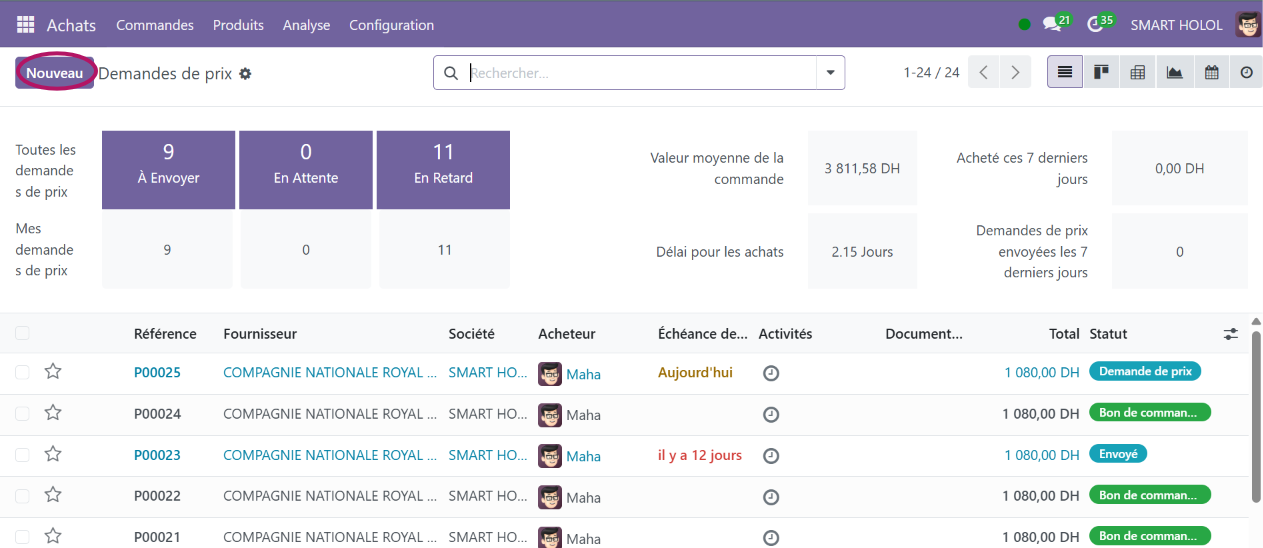
\includegraphics[width=\linewidth]{image/Achat/Achat2.png}
\caption{Liste des demandes de prix}
\label{fig:achat2}
\end{figure}

Renseigner les informations nécessaires, notamment le fournisseur et les produits ou services concernés, puis enregistrer la demande. Il est ensuite possible d'imprimer la demande de prix au format PDF.

\begin{figure}[H]
\centering
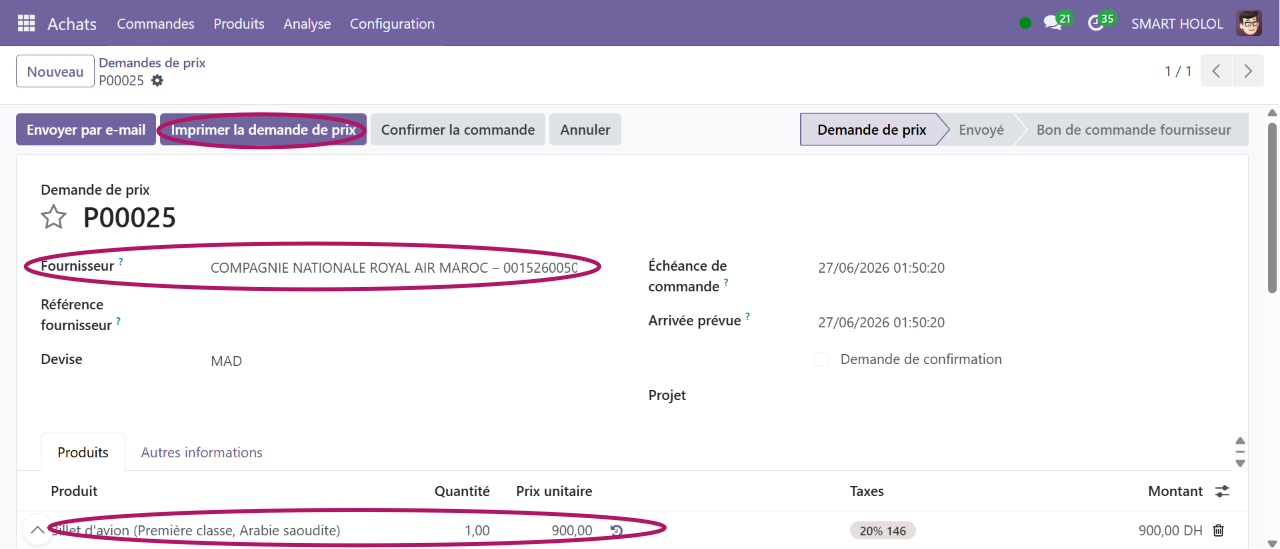
\includegraphics[width=\linewidth]{image/Achat/Achat3.png}
\caption{Création d'une nouvelle demande de prix}
\label{fig:achat3}
\end{figure}

\begin{figure}[H]
\centering
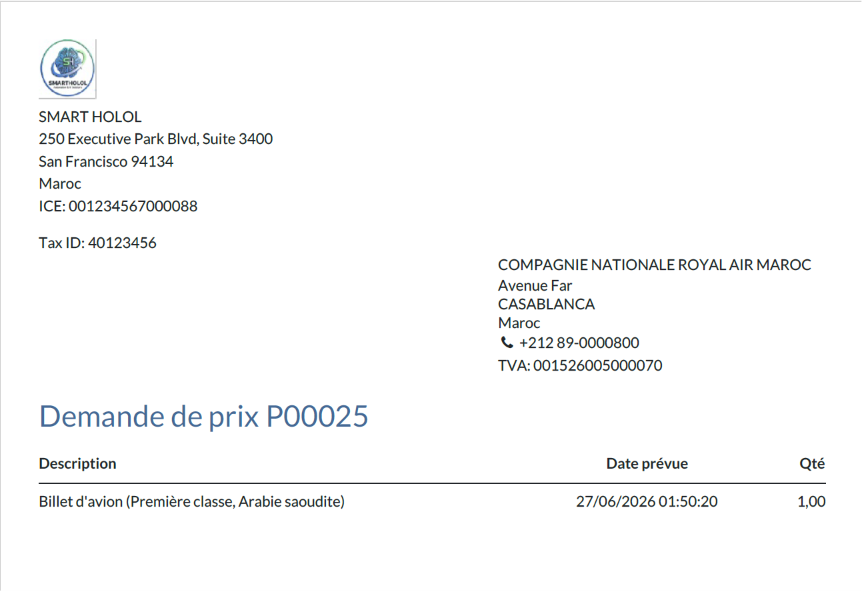
\includegraphics[width=\linewidth]{image/Achat/Achat4.png}
\caption{Exemple d'une demande de prix générée au format PDF}
\label{fig:achat4}
\end{figure}

Une fois la demande validée par le fournisseur, il suffit de cliquer sur \textbf{Confirmer la commande} afin de la transformer en bon de commande.

\begin{figure}[H]
\centering
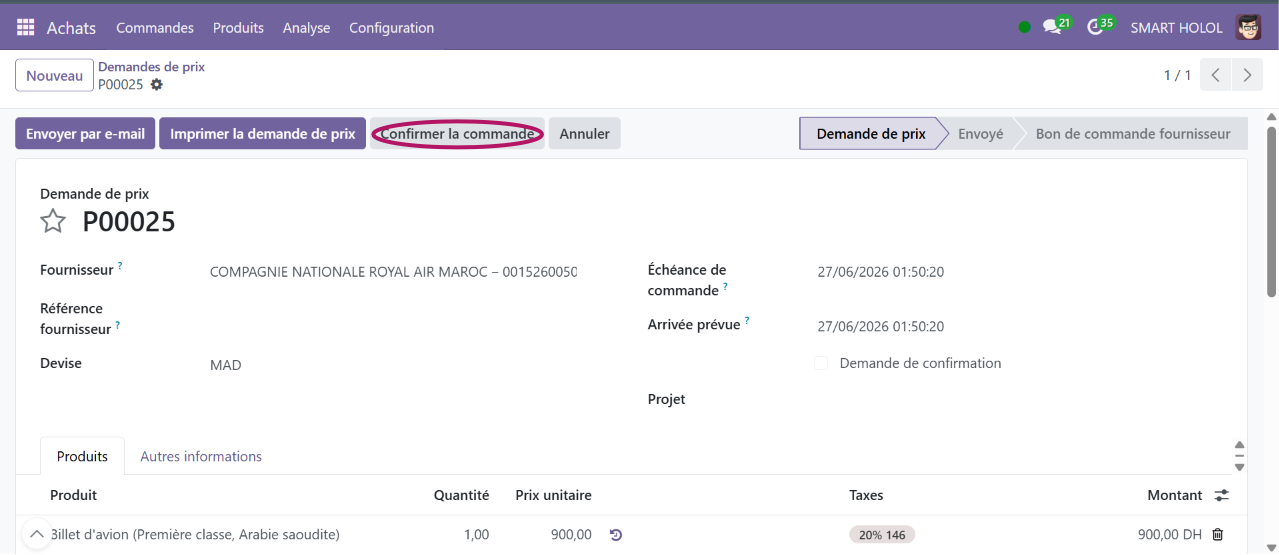
\includegraphics[width=\linewidth]{image/Achat/Achat5.png}
\caption{Confirmation de la commande fournisseur}
\label{fig:achat5}
\end{figure}

Après la confirmation, Odoo propose différentes actions permettant de poursuivre le processus d'achat, telles que la création de la facture fournisseur, l'envoi du bon de commande par e-mail ou encore la confirmation de la réception des produits ou services.

\begin{figure}[H]
\centering
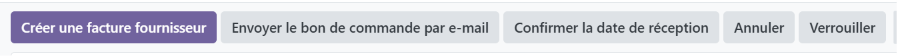
\includegraphics[width=\linewidth]{image/Achat/Achat6.png}
\caption{Actions disponibles après la confirmation de la commande}
\label{fig:achat6}
\end{figure}
\section{CONTRÔLE DES COÛTS}

Le contrôle des coûts est assuré grâce au rapprochement manuel entre le bon de commande fournisseur, la confirmation de réservation (ou de prestation) et la facture reçue du prestataire. Cette vérification permet de s'assurer que les prestations fournies, les quantités et les tarifs correspondent à ceux qui ont été commandés avant la validation de la facture. Contrairement à l'édition Enterprise, Odoo Community ne dispose pas nativement du mécanisme de contrôle à trois voies (\textit{3-Way Matching}). La cohérence des informations est donc vérifiée manuellement avant la validation de la facture fournisseur.

La première étape consiste à créer un devis client. Pour cela, accéder au module \textbf{Ventes}, puis sélectionner le menu \textbf{Commandes > Devis}.

\begin{figure}[H]
\centering
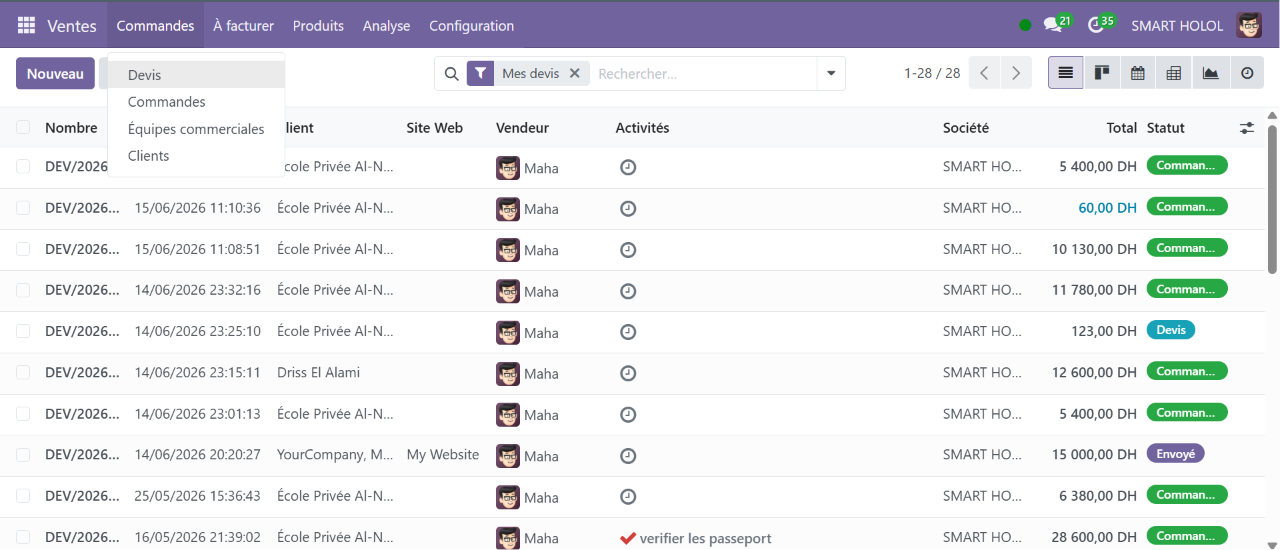
\includegraphics[width=\linewidth]{image/Achat/Vente1.png}
\caption{Accès à la liste des devis dans le module Ventes}
\label{fig:vente1}
\end{figure}

Cliquer sur \textbf{Nouveau} afin de créer un nouveau devis.

\begin{figure}[H]
\centering
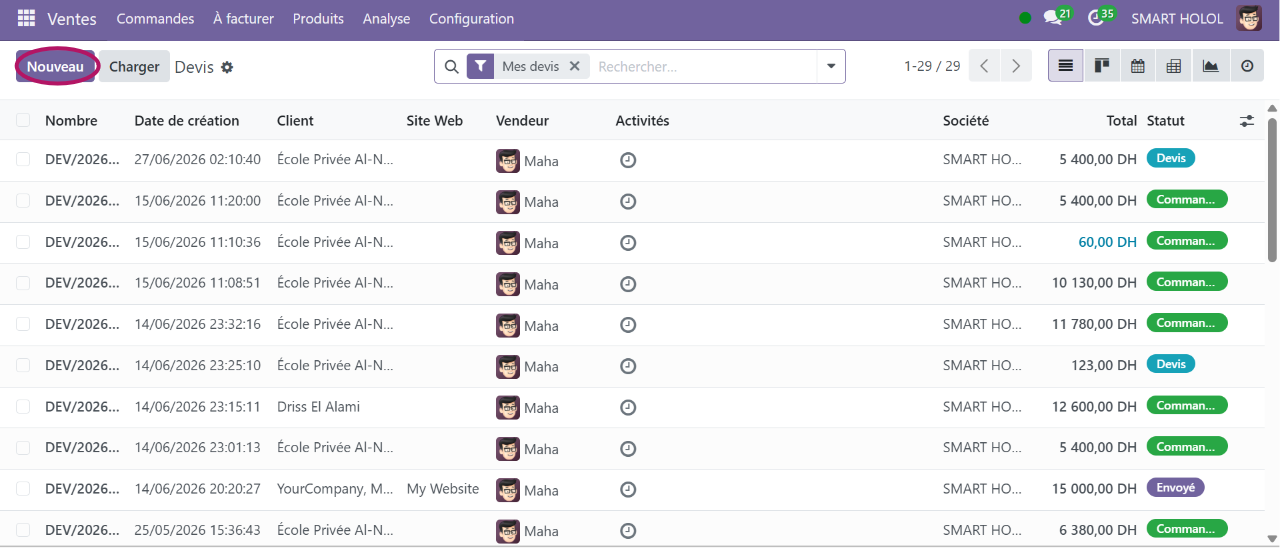
\includegraphics[width=\linewidth]{image/Achat/Vente.png}
\caption{Création d'un nouveau devis}
\label{fig:vente2}
\end{figure}

Renseigner les informations du client ainsi que les produits ou services concernés.

\begin{figure}[H]
\centering
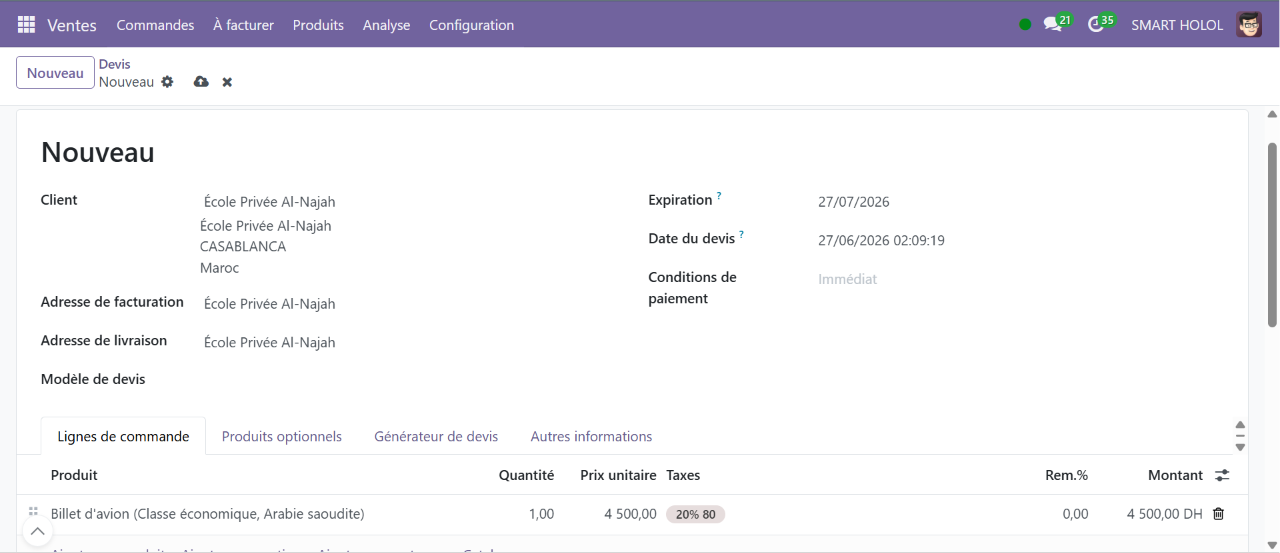
\includegraphics[width=\linewidth]{image/Achat/Vente2.png}
\caption{Remplissage du devis client}
\label{fig:vente3}
\end{figure}

Ensuite, accéder au module \textbf{Achats}, puis au menu \textbf{Commandes > Bons de commande} afin de créer une commande fournisseur correspondant au devis.

\begin{figure}[H]
\centering
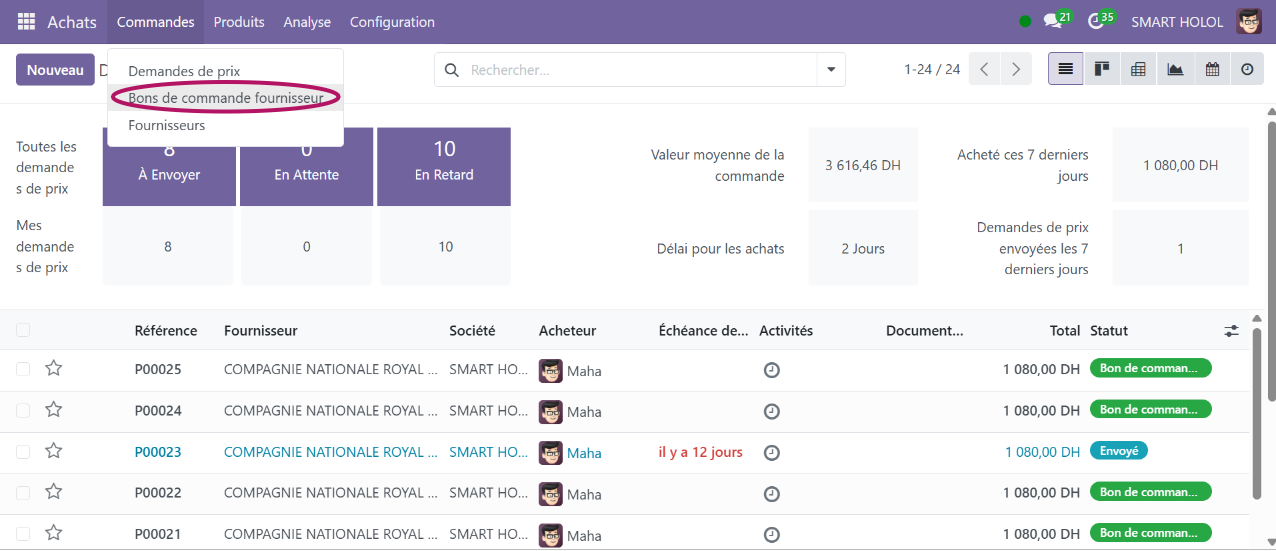
\includegraphics[width=\linewidth]{image/Achat/Vente3.png}
\caption{Accès aux bons de commande fournisseurs}
\label{fig:vente4}
\end{figure}

Cliquer sur \textbf{Nouveau} pour créer un bon de commande fournisseur.

\begin{figure}[H]
\centering
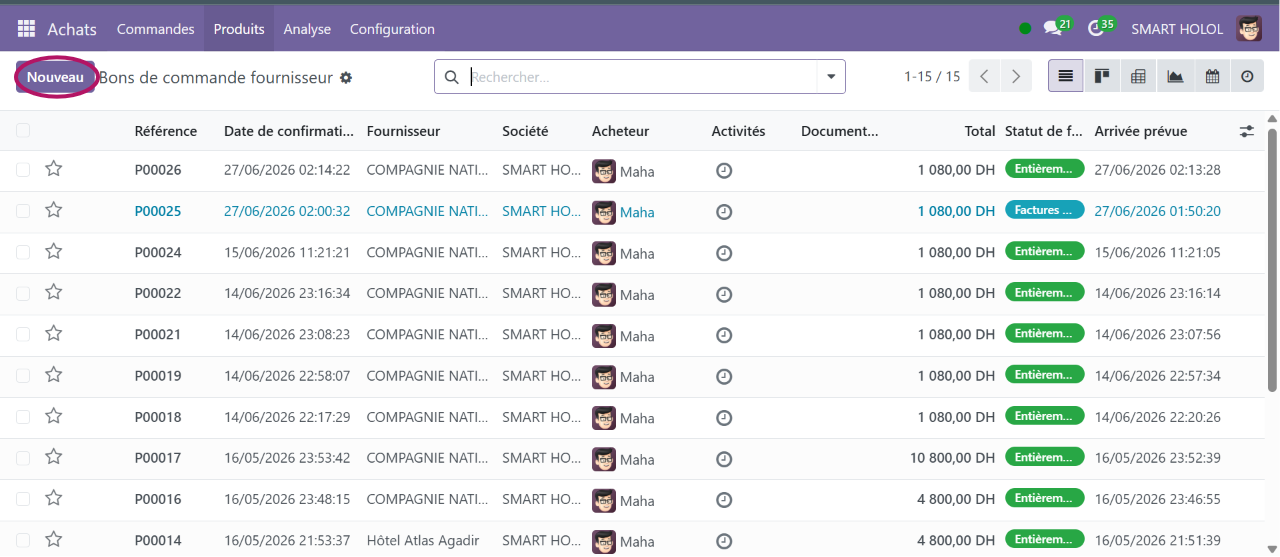
\includegraphics[width=\linewidth]{image/Achat/Vente5.png}
\caption{Création d'un nouveau bon de commande fournisseur}
\label{fig:vente5}
\end{figure}

Le produit (ou service) ainsi que la quantité doivent être identiques à ceux indiqués dans le devis client afin d'assurer la cohérence entre les documents.

\begin{figure}[H]
\centering
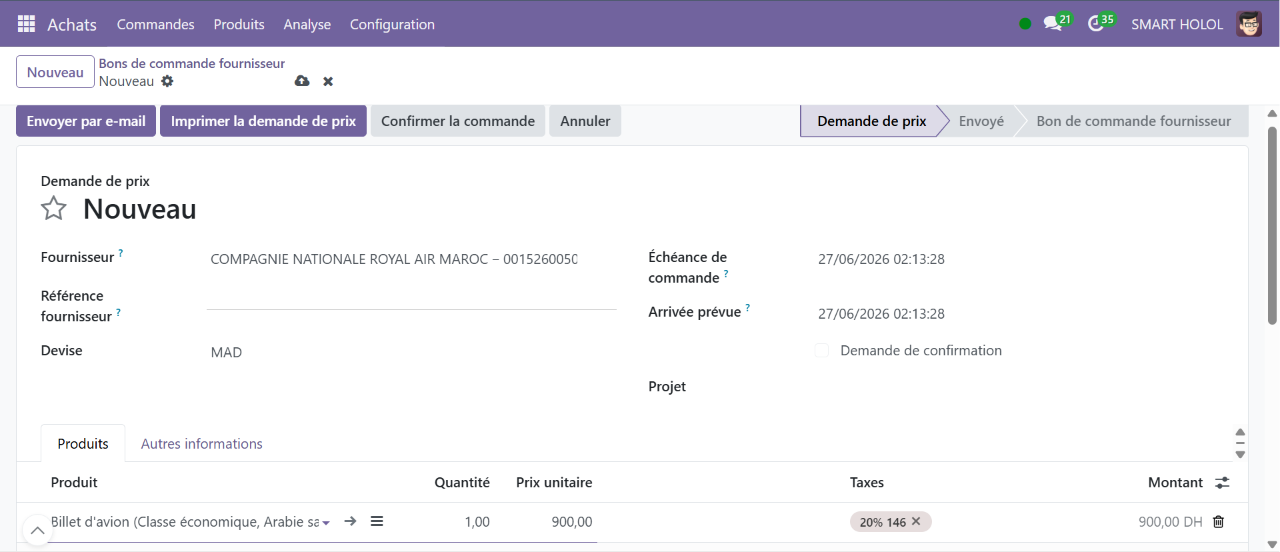
\includegraphics[width=\linewidth]{image/Achat/Vente4.png}
\caption{Correspondance entre le devis client et le bon de commande fournisseur}
\label{fig:vente6}
\end{figure}

Après vérification des informations, confirmer le bon de commande.

\begin{figure}[H]
\centering
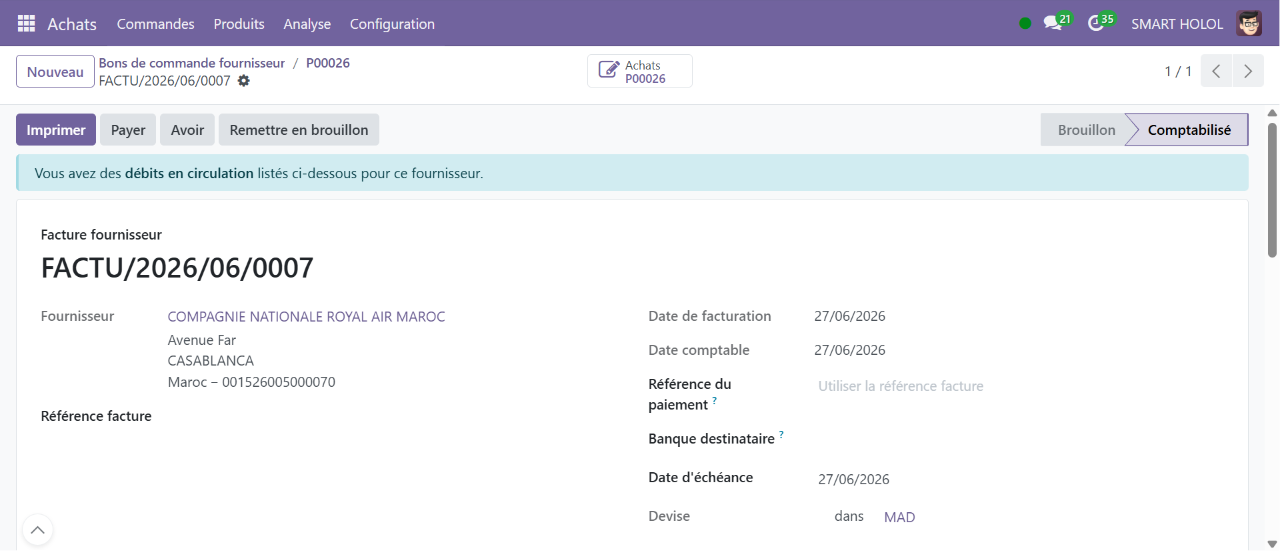
\includegraphics[width=\linewidth]{image/Achat/Vente6.png}
\caption{Confirmation du bon de commande fournisseur}
\label{fig:vente7}
\end{figure}

Une fois le bon de commande confirmé, Odoo affiche un ruban d'information indiquant les opérations en attente, notamment les débits ou les factures fournisseurs associés. Ce ruban facilite le suivi des documents liés à la commande.

Lorsque le prestataire transmet la confirmation de réservation (ou de la prestation), celle-ci est conservée comme pièce justificative. À la réception de la facture fournisseur, cette dernière est enregistrée dans Odoo.

L'utilisateur effectue ensuite un rapprochement manuel entre le bon de commande, la confirmation de réservation et la facture fournisseur en vérifiant la cohérence des quantités, des prestations et des tarifs. En cas d'écart, la facture fournisseur n'est pas validée tant qu'une régularisation n'a pas été effectuée par le prestataire.



%=================================================
% MODULE DOSSIER DE VOYAGE
%=================================================
\chapter{Module DOSSIER DE VOYAGE}
\section{LOGISTIQUE CLIENT}

La création automatique d'un dossier logistique (dossier de voyage sous forme de projet et de tâches) est assurée dès la confirmation du devis commercial. Grâce au lien natif entre les modules \textbf{Ventes} et \textbf{Projets} d'Odoo, la confirmation d'une ligne correspondant à un service de voyage (par exemple un circuit touristique) génère automatiquement un projet ainsi que les tâches associées afin d'assurer le suivi des démarches administratives du client.

Dans un premier temps, accéder au module \textbf{Ventes}.

\begin{figure}[H]
\centering
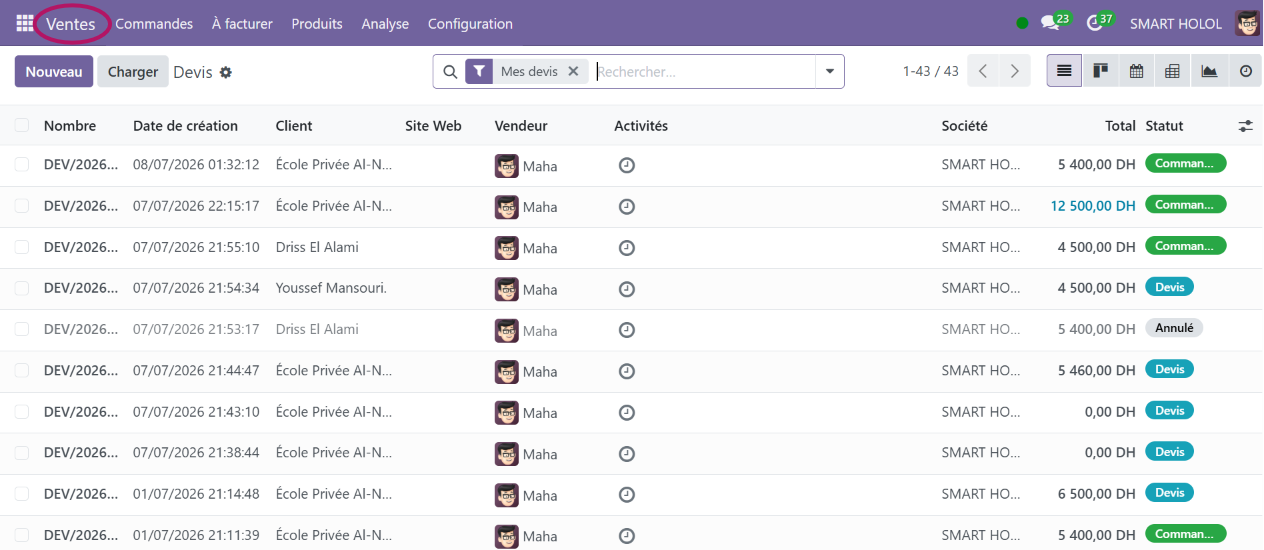
\includegraphics[width=\linewidth]{image/DOSSIERS DE VOYAGE/vente0.png}
\caption{Accès au module Achats}
\label{fig:logistique1}
\end{figure}

Depuis le menu \textbf{Produits}, sélectionner \textbf{Produits}.

\begin{figure}[H]
\centering
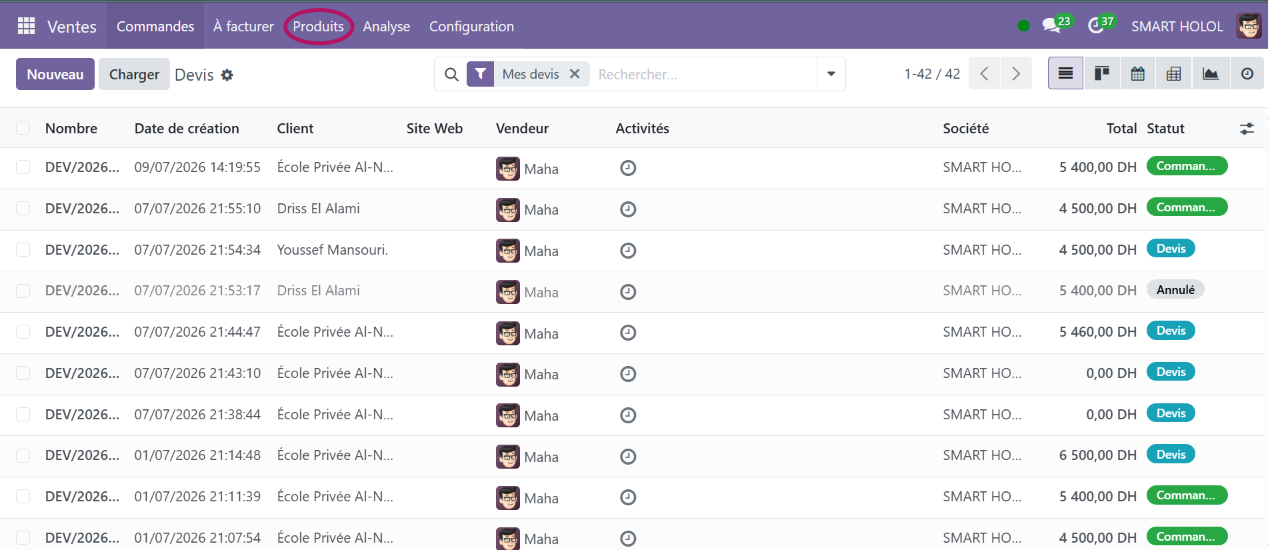
\includegraphics[width=\linewidth]{image/DOSSIERS DE VOYAGE/vente1.2.png}
\caption{Menu Produits}
\label{fig:logistique2}
\end{figure}

\begin{figure}[H]
\centering
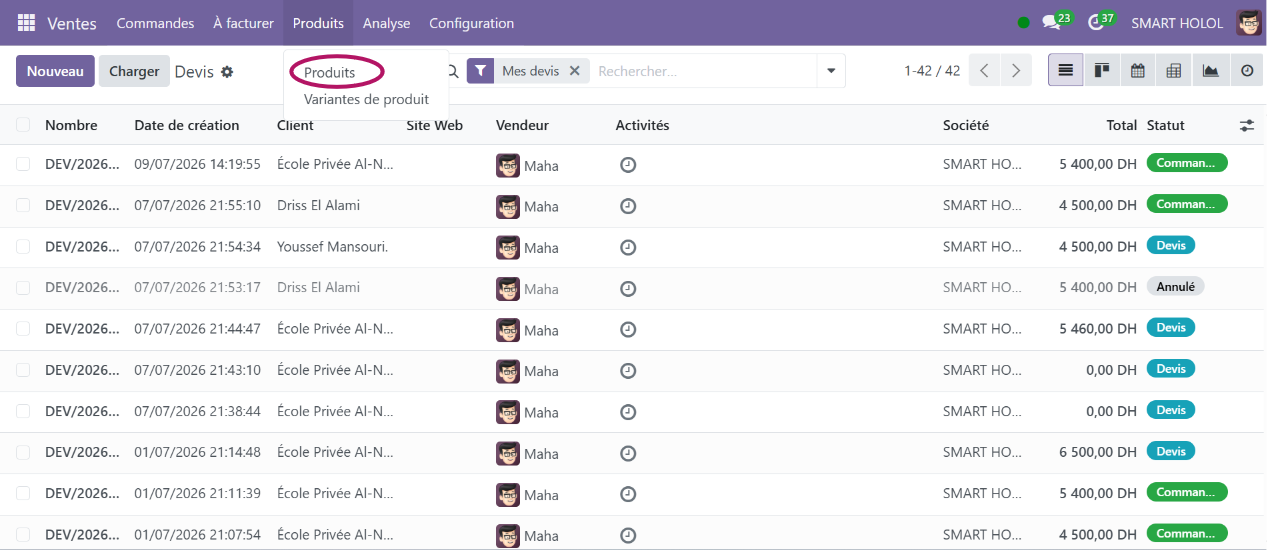
\includegraphics[width=\linewidth]{image/DOSSIERS DE VOYAGE/vente1.0.png}
\caption {Produits produits}
\label{fig:logistique3}
\end{figure}

\begin{figure}[H]
\centering
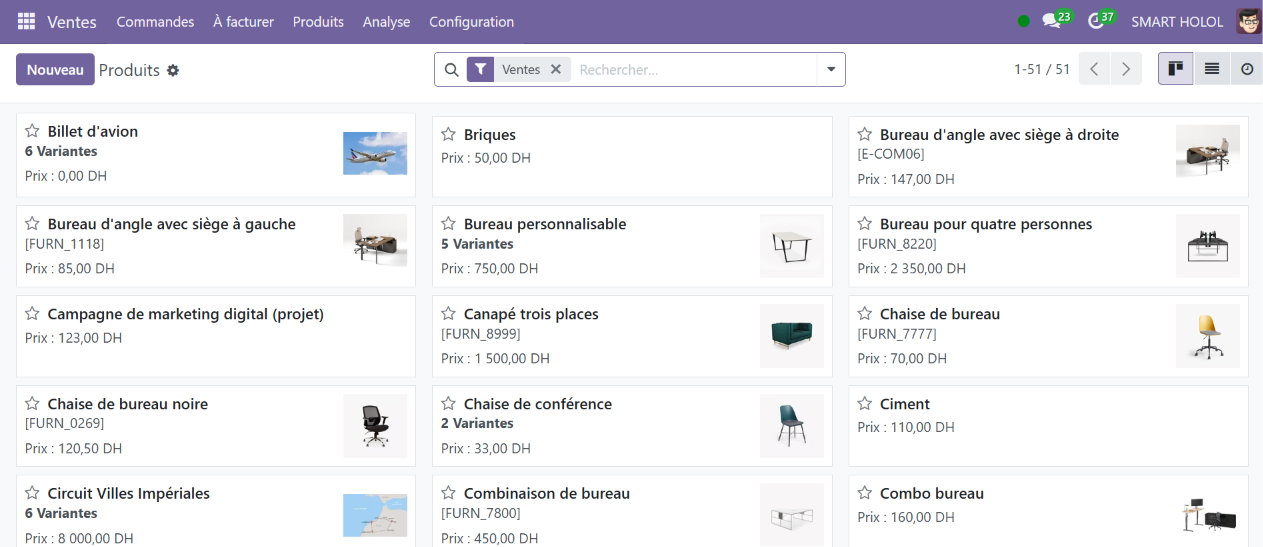
\includegraphics[width=\linewidth]{image/DOSSIERS DE VOYAGE/liste_produits.png}
\caption{Liste des produit}
\label{fig:logistique4}
\end{figure}

Choisir un produit puis le configurer avec les paramètres suivants :
\begin{itemize}
    \item \textbf{Type de produit} : Service ;
    \item \textbf{Créer à la commande} : Projet \& tâche ;
    \item \textbf{Politique de facturation} : Basée sur les jalons.
\end{itemize}



\begin{figure}[H]
\centering
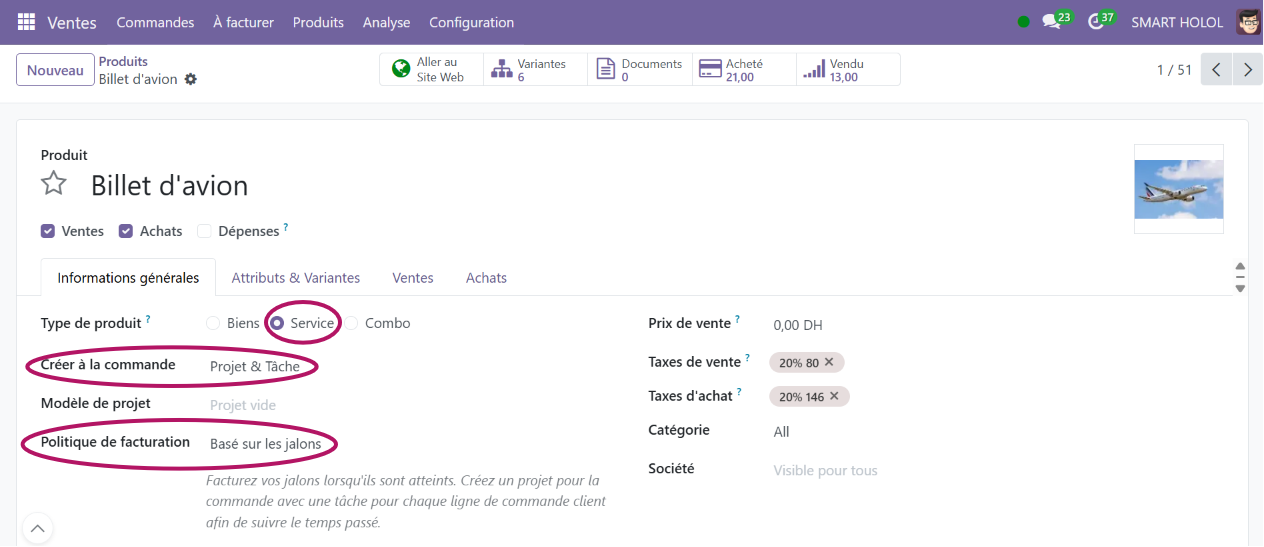
\includegraphics[width=\linewidth]{image/DOSSIERS DE VOYAGE/vente1.3.png}
\caption{Accès au module Ventes}
\label{fig:logistique5}
\end{figure}



Depuis le module \textbf{Ventes}, accéder au menu \textbf{Commandes}.
\begin{figure}[H]
\centering
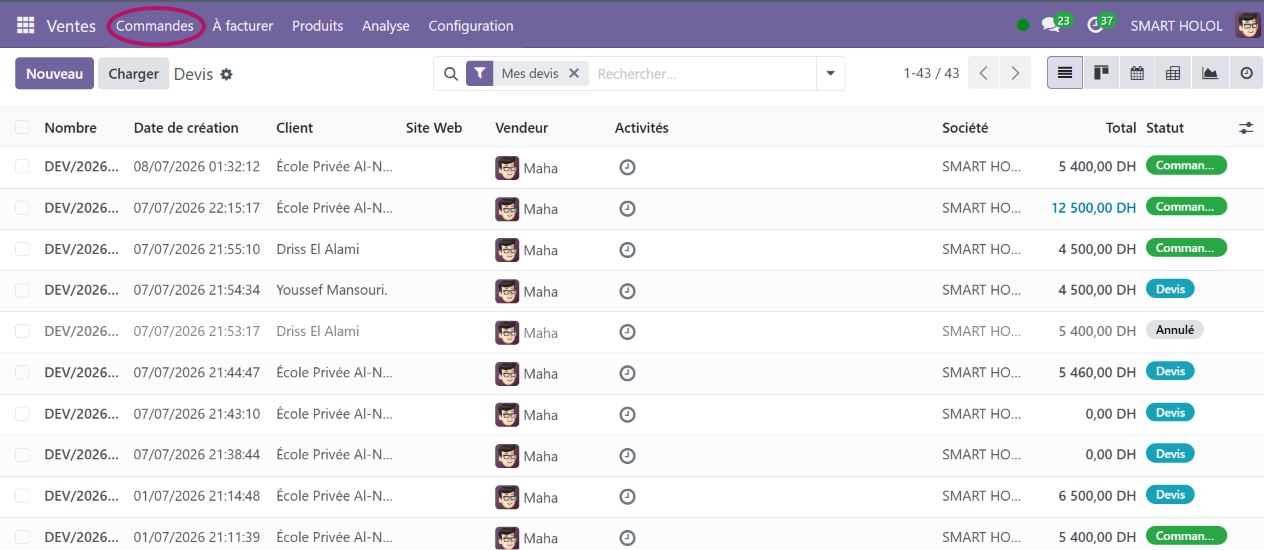
\includegraphics[width=\linewidth]{image/DOSSIERS DE VOYAGE/vente1.png}
\caption{Menu Commandes}
\label{fig:logistique7}
\end{figure}


\begin{figure}[H]
\centering

\includegraphics[width=\linewidth]{image/DOSSIERS DE VOYAGE/Vente2.png}
\caption{Menu Commandes}
\label{fig:logistique8}
\end{figure}

Créer un nouveau devis en cliquant sur \textbf{Nouveau}.

\begin{figure}[H]
\centering
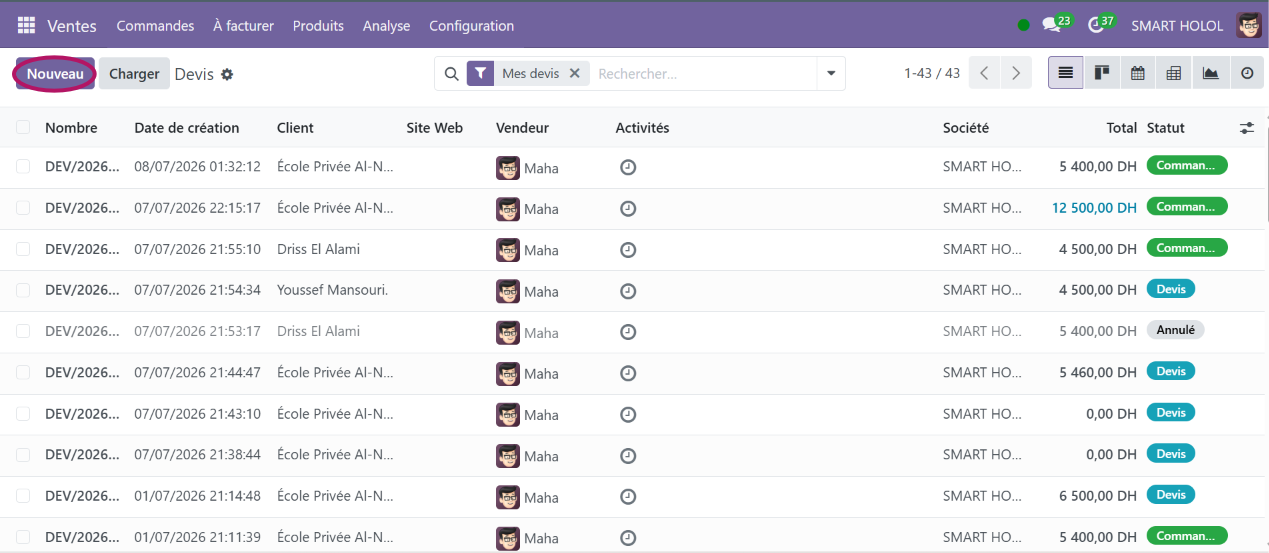
\includegraphics[width=\linewidth]{image/DOSSIERS DE VOYAGE/vente3.png}
\caption{Nouveau devis}
\label{fig:logistique9}
\end{figure}

Sélectionner le produit précédemment configuré.

\begin{figure}[H]
\centering

\includegraphics[width=\linewidth]{image/DOSSIERS DE VOYAGE/Vente4.png}
\caption{Sélection du produit}
\label{fig:logistique10}
\end{figure}

Enregistrer le devis.

\begin{figure}[H]
\centering

\includegraphics[width=\linewidth]{image/DOSSIERS DE VOYAGE/Vente5.png}
\caption{Enregistrement du devis}
\label{fig:logistique11}
\end{figure}

Confirmer ensuite le devis.

\begin{figure}[H]
\centering
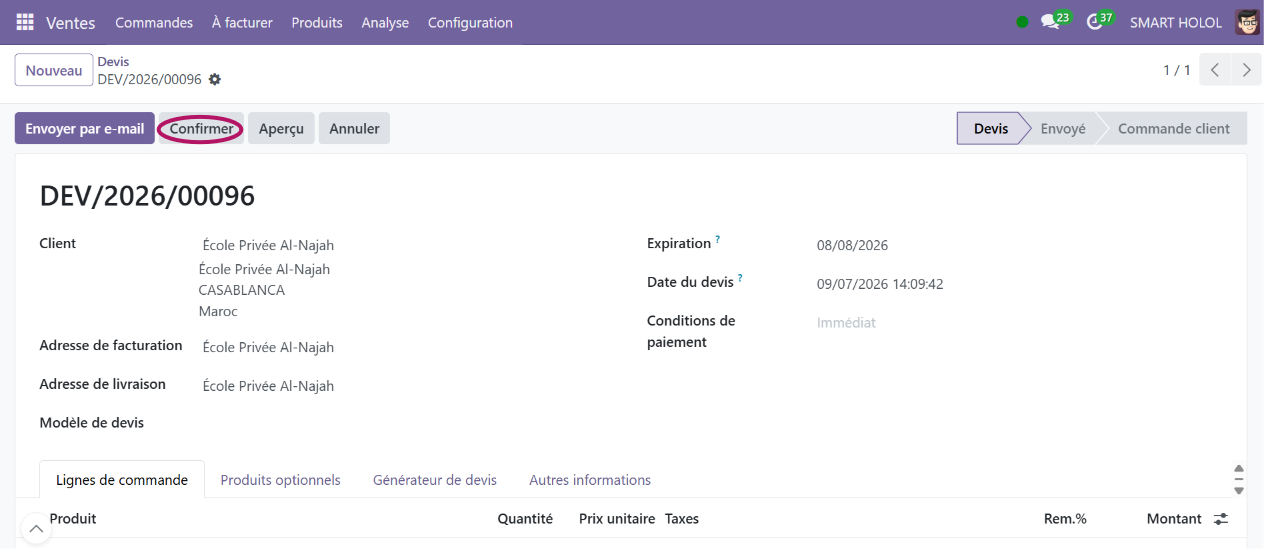
\includegraphics[width=\linewidth]{image/DOSSIERS DE VOYAGE/vente6.png}
\caption{Confirmation du devis}
\label{fig:logistique12}
\end{figure}

Enfin, accéder au module \textbf{Projets}.

\begin{figure}[H]
\centering
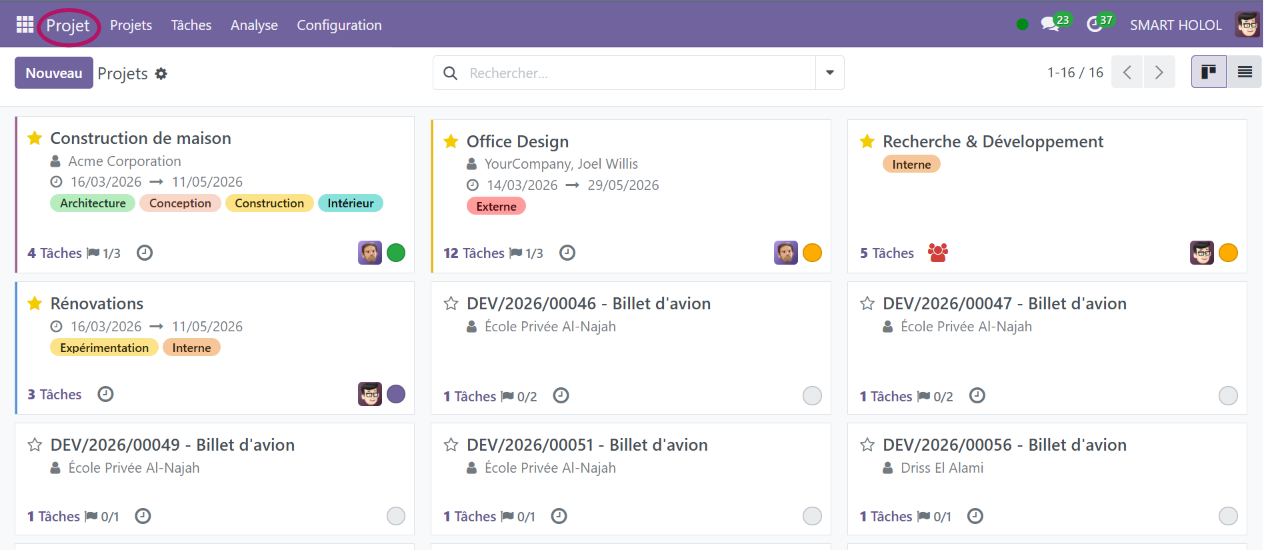
\includegraphics[width=\linewidth]{image/DOSSIERS DE VOYAGE/Projet0.png}
\caption{Accès au module Projets}
\label{fig:logistique13}
\end{figure}

Le dossier de voyage est automatiquement créé sous la forme d'un projet contenant les tâches associées.

\begin{figure}[H]
\centering
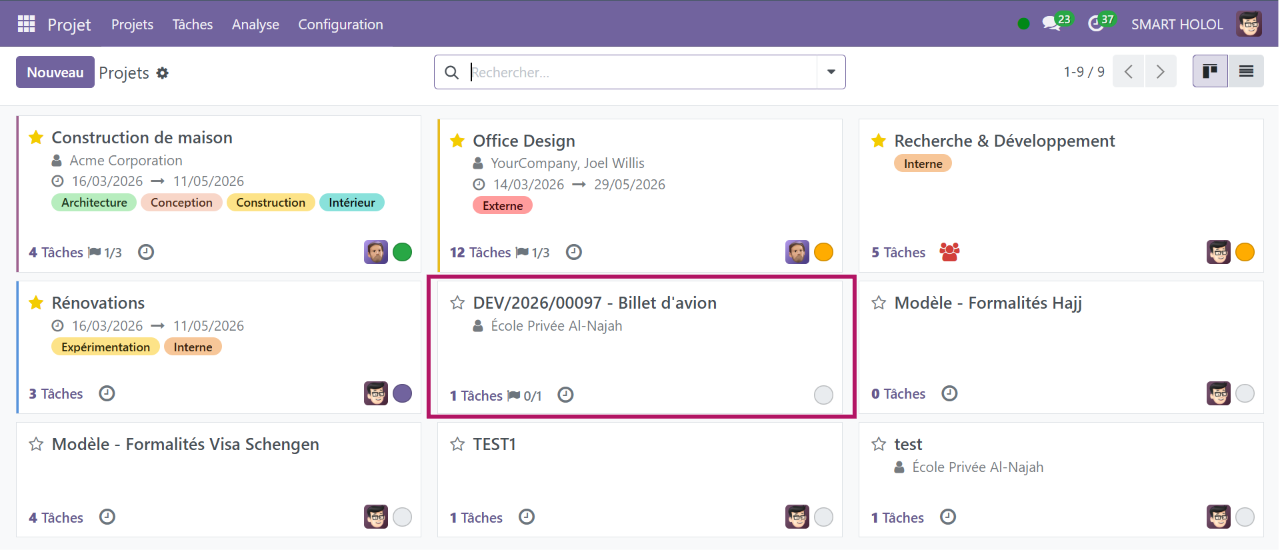
\includegraphics[width=\linewidth]{image/DOSSIERS DE VOYAGE/Projet1.png}
\caption{Création automatique du dossier de voyage}
\label{fig:logistique14}
\end{figure}

\section{SUIVI ADMINISTRATIF}

Le suivi des check-lists opérationnelles de chaque dossier client (obtention du visa, émission des billets d'avion, confirmation des vouchers, paiement de l'assurance, etc.) est réalisé à l'aide des fonctionnalités du module \textbf{Projets} d'Odoo. Les tâches et leurs différentes étapes permettent de suivre l'avancement des démarches administratives et de s'assurer que chaque collaborateur accomplit les actions qui lui sont attribuées dans les délais.

Accéder au module \textbf{Projets}.

\begin{figure}[H]
\centering
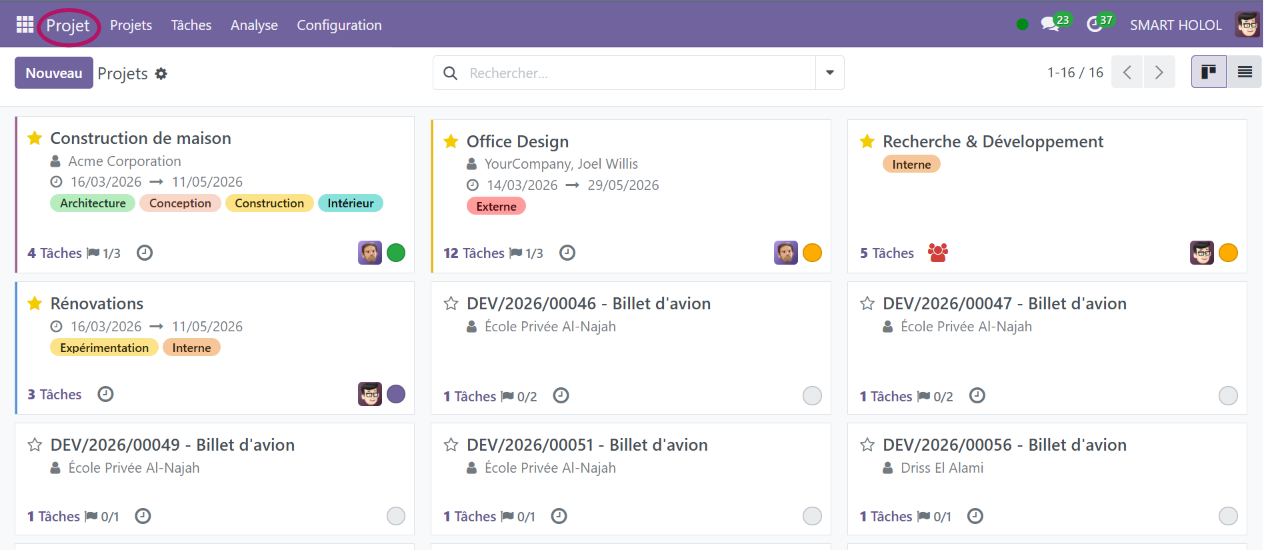
\includegraphics[width=\linewidth]{image/DOSSIERS DE VOYAGE/Projet0.png}
\caption{Accès au module Projets}
\label{fig:suivi1}
\end{figure}

Cliquer sur \textbf{Nouveau} pour créer un projet.

\begin{figure}[H]
\centering
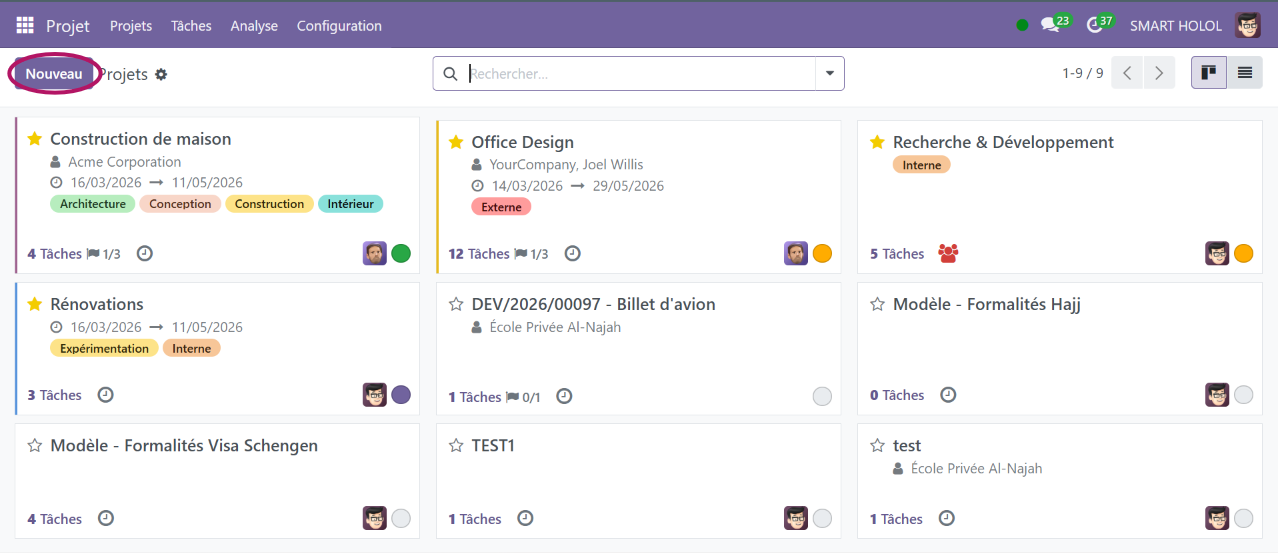
\includegraphics[width=\linewidth]{image/DOSSIERS DE VOYAGE/Projet2.png}
\caption{Création d'un nouveau projet}
\label{fig:suivi2}
\end{figure}

Renseigner les informations du projet.

\begin{figure}[H]
\centering
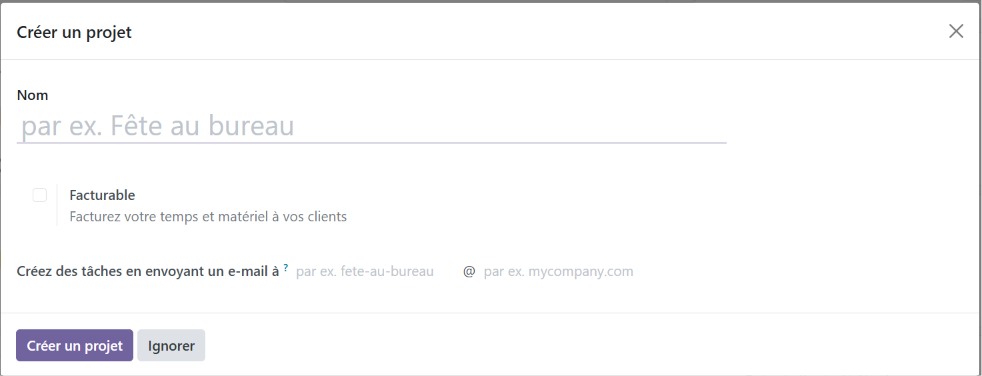
\includegraphics[width=\linewidth]{image/DOSSIERS DE VOYAGE/Projet3.png}
\caption{Configuration du projet}
\label{fig:suivi3}
\end{figure}

Ajouter les différentes étapes permettant d'assurer le suivi de chaque tâche.

\begin{figure}[H]
\centering
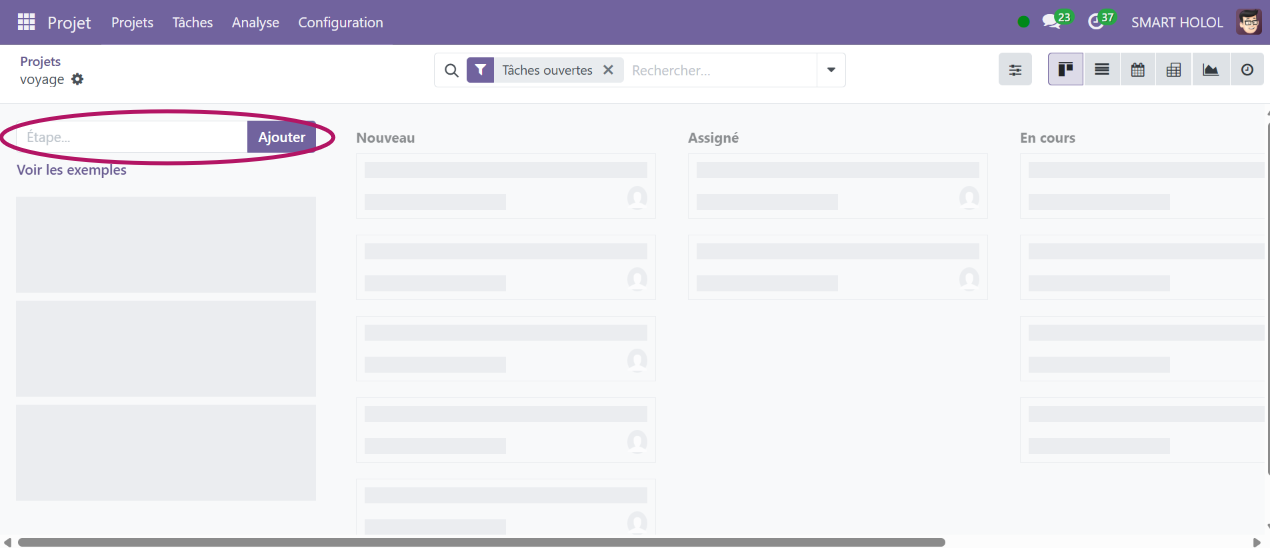
\includegraphics[width=\linewidth]{image/DOSSIERS DE VOYAGE/Projet4.png}
\caption{Création des étapes du projet}
\label{fig:suivi4}
\end{figure}

\begin{figure}[H]
\centering
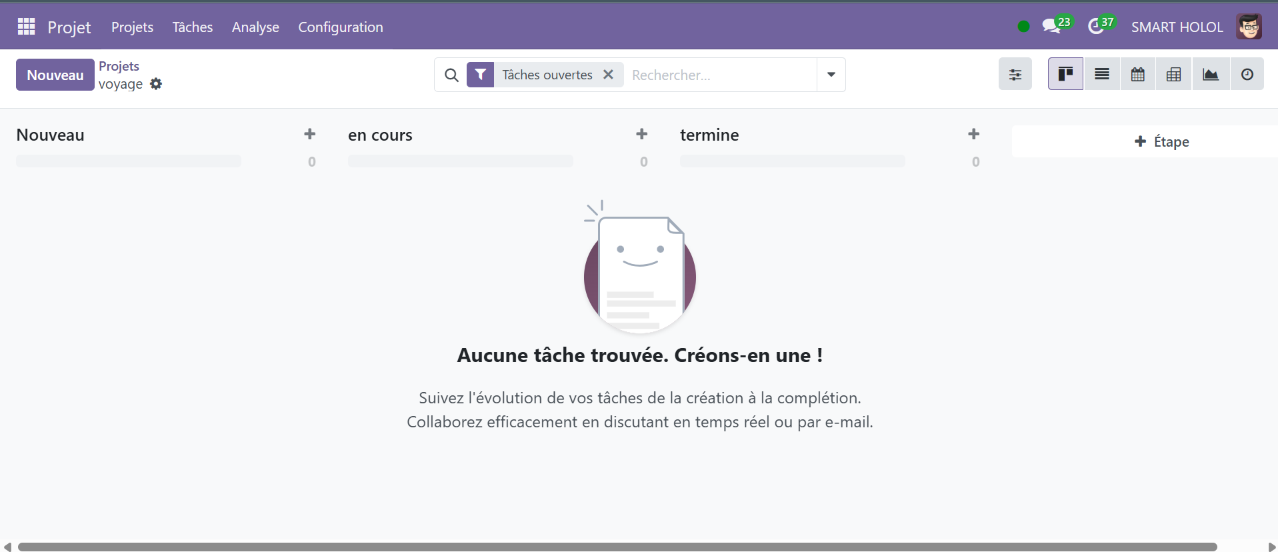
\includegraphics[width=\linewidth]{image/DOSSIERS DE VOYAGE/Projet5.png}
\caption{Organisation des étapes du projet}
\label{fig:suivi5}
\end{figure}

Créer les tâches correspondant aux différentes opérations administratives et les affecter aux collaborateurs responsables.

\begin{figure}[H]
\centering
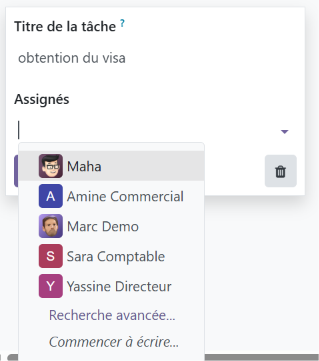
\includegraphics[width=\linewidth]{image/DOSSIERS DE VOYAGE/Projet6.png}
\caption{Création et affectation des tâches}
\label{fig:suivi6}
\end{figure}

Le suivi de l'avancement est ensuite réalisé en déplaçant les tâches d'une étape à une autre jusqu'à leur finalisation.

\begin{figure}[H]
\centering
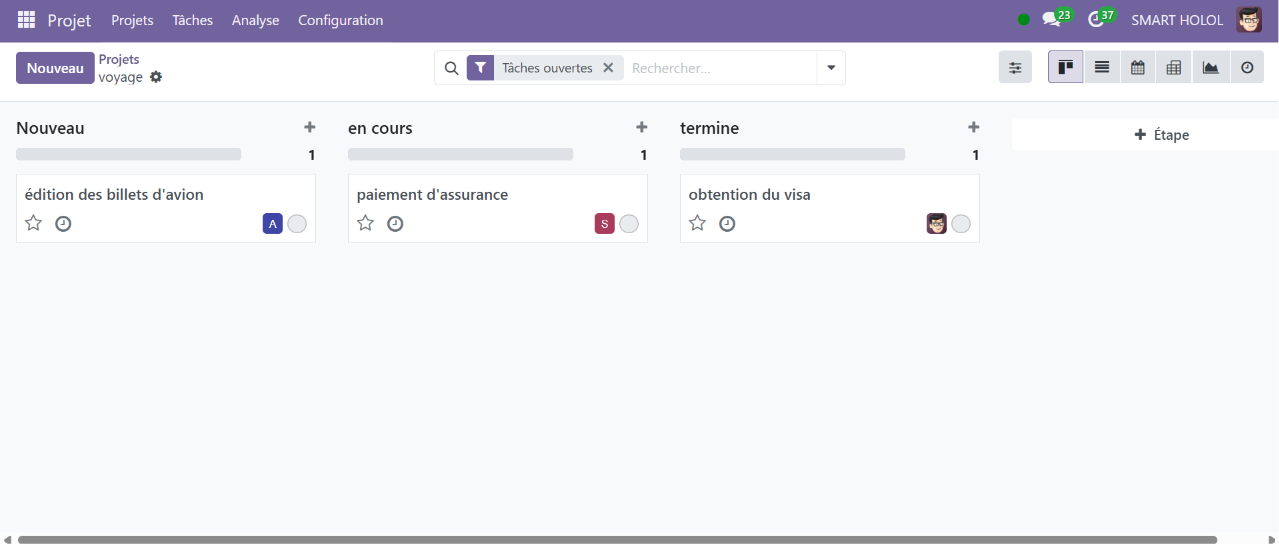
\includegraphics[width=\linewidth]{image/DOSSIERS DE VOYAGE/Projet7.png}
\caption{Suivi de l'avancement des tâches}
\label{fig:suivi7}
\end{figure}

\section{GESTION DOCUMENTAIRE}
La centralisation des documents des passagers (photocopies de passeports, formulaires d'assurance, billets d'avion, etc.) est assurée grâce au \textbf{chatter} intégré à toutes les fiches d'Odoo (CRM, Ventes et Projets). Cette fonctionnalité permet de joindre des documents directement à une tâche, de mentionner des collaborateurs et de conserver un historique complet des échanges et des pièces jointes.

Accéder au module \textbf{Projets}.

\begin{figure}[H]
\centering
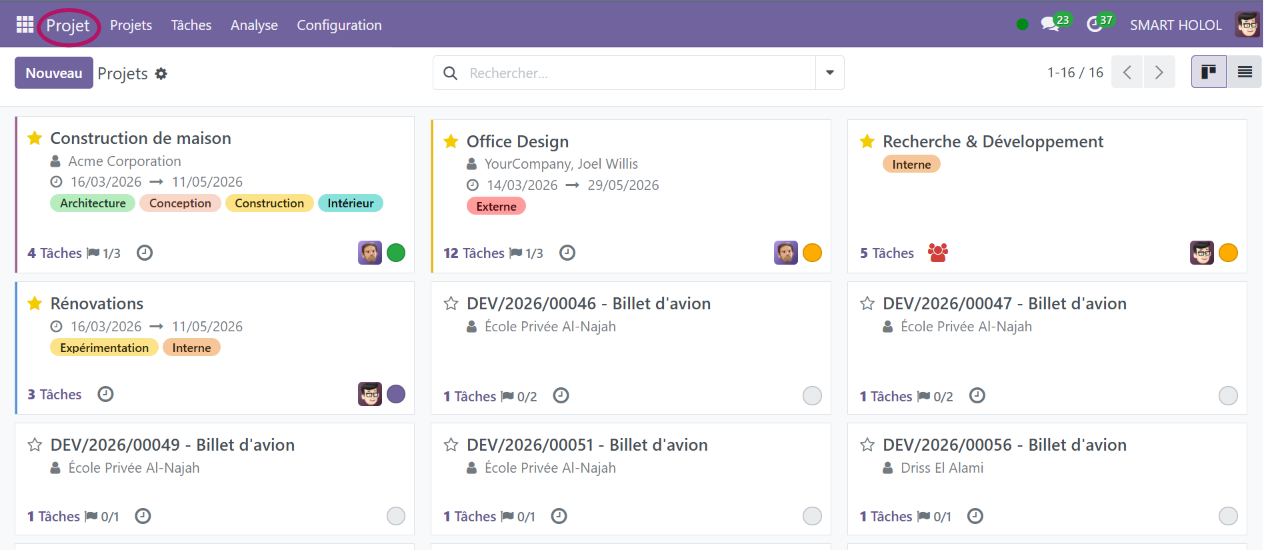
\includegraphics[width=\linewidth]{image/DOSSIERS DE VOYAGE/Projet0.png}
\caption{Accès au module Projets}
\label{fig:documents1}
\end{figure}

Sélectionner le projet correspondant au dossier client.

\begin{figure}[H]
\centering
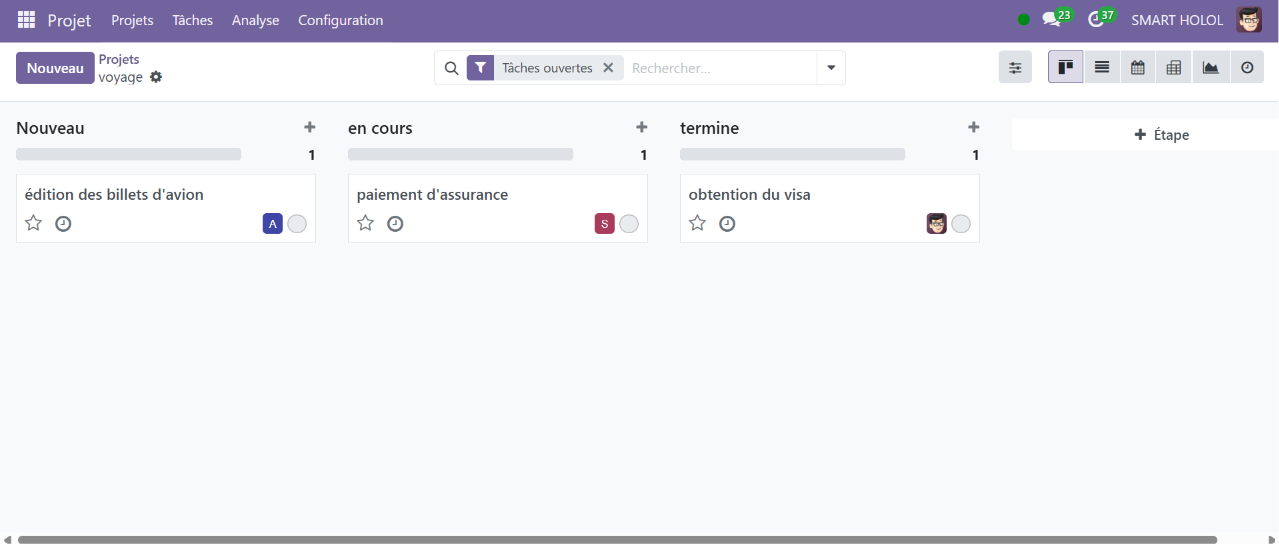
\includegraphics[width=\linewidth]{image/DOSSIERS DE VOYAGE/Projet7.png}
\caption{Sélection du projet}
\label{fig:documents2}
\end{figure}

Ouvrir la tâche concernée.

\begin{figure}[H]
\centering
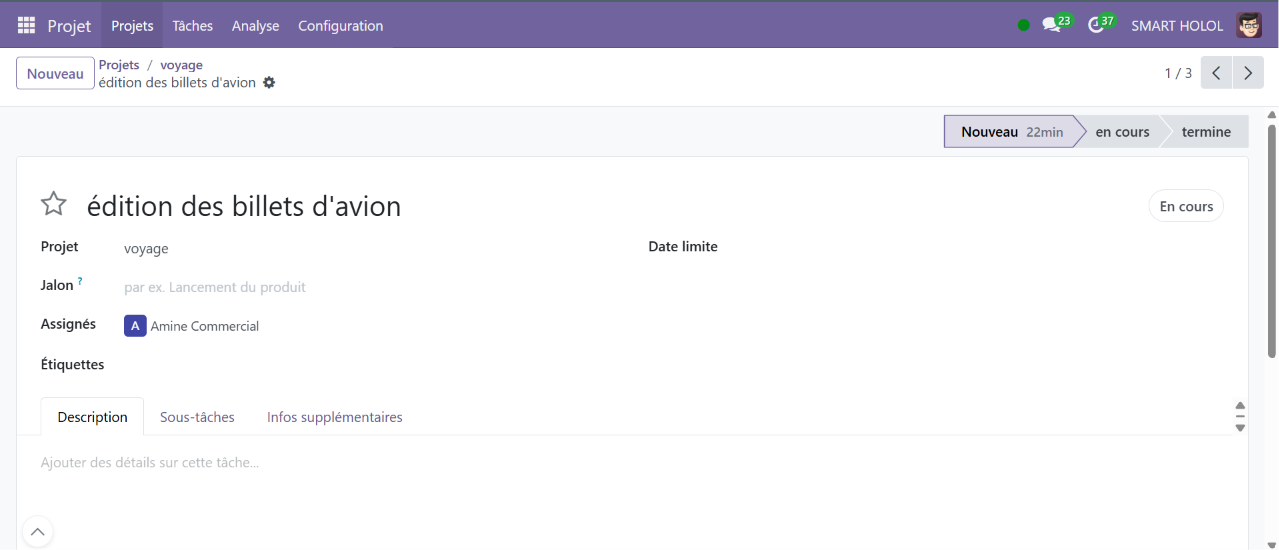
\includegraphics[width=\linewidth]{image/DOSSIERS DE VOYAGE/Projet8.png}
\caption{Sélection d'une tâche}
\label{fig:documents3}
\end{figure}

Accéder au \textbf{chatter}, situé dans la partie inférieure de la fiche de la tâche.

\begin{figure}[H]
\centering
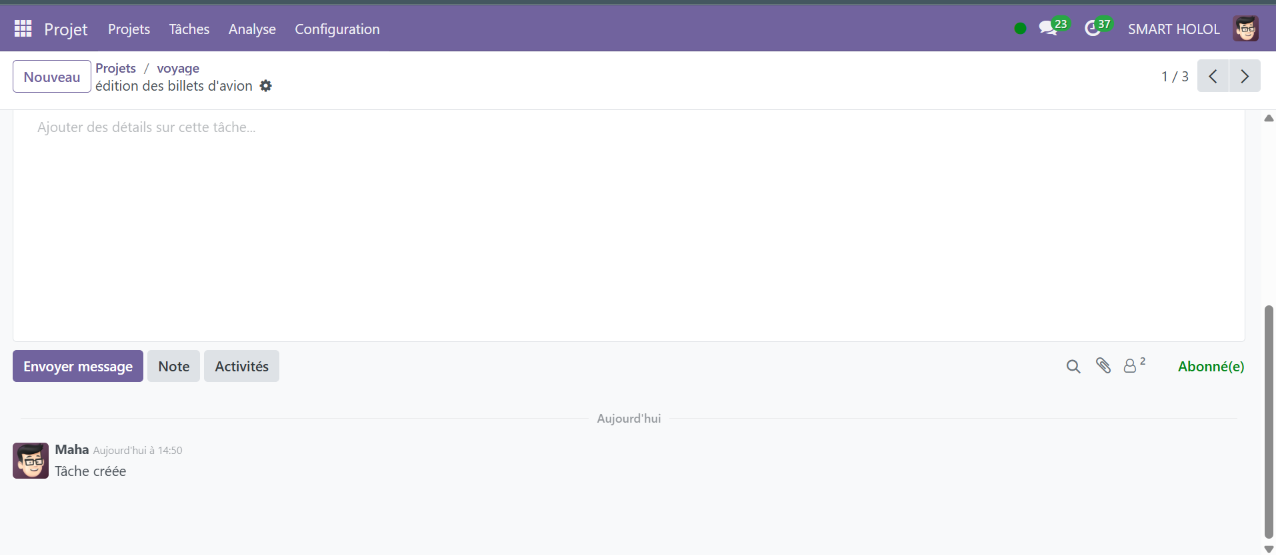
\includegraphics[width=\linewidth]{image/DOSSIERS DE VOYAGE/Projet9.png}
\caption{Accès au chatter}
\label{fig:documents4}
\end{figure}

Cliquer sur \textbf{Joindre un fichier} afin d'ajouter les documents nécessaires au dossier du client.

\begin{figure}[H]
\centering
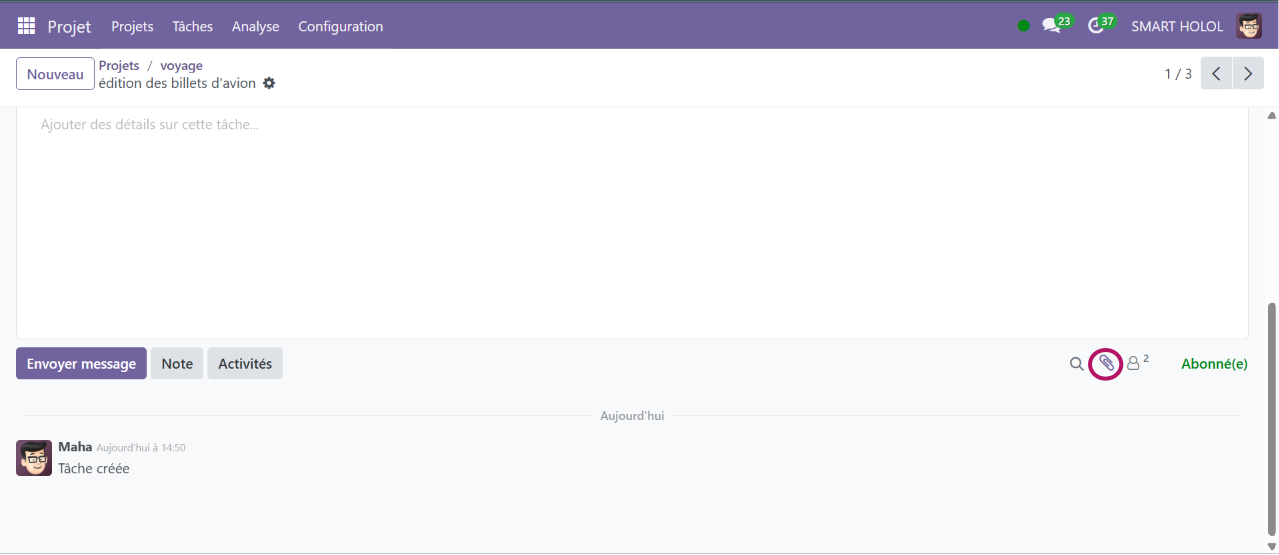
\includegraphics[width=\linewidth]{image/DOSSIERS DE VOYAGE/Projet10.png}
\caption{Ajout d'une pièce jointe}
\label{fig:documents5}
\end{figure}

Les documents sont alors enregistrés dans le chatter et restent accessibles à l'ensemble des collaborateurs autorisés, garantissant ainsi la centralisation et la traçabilité des pièces jointes.

\begin{figure}[H]
\centering
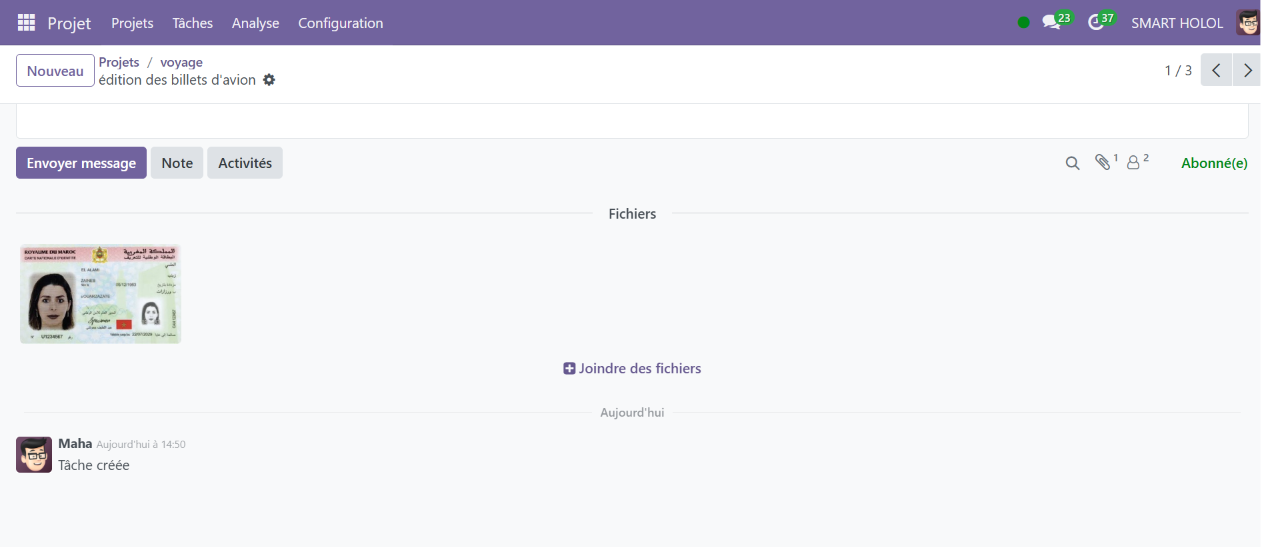
\includegraphics[width=\linewidth]{image/DOSSIERS DE VOYAGE/Projet11.png}
\caption{Historique des documents dans le chatter}
\label{fig:documents6}
\end{figure}

%=================================================
% MODULE SITE WEB
%=================================================
\chapter{Module SITE WEB}
\section{PRÉSENTATION DE L'OFFRE}

L'agence met à disposition une vitrine web moderne permettant de présenter les différents packages de voyage (séjours balnéaires, treks nature, circuits de découverte, etc.). Chaque offre est accompagnée d'une description détaillée, de photographies attractives et des informations essentielles permettant aux visiteurs de découvrir facilement les prestations proposées.

Le module \textbf{Website/eCommerce} d'Odoo Community constitue une solution complète pour la création et la gestion de cette vitrine. Il intègre un éditeur visuel en glisser-déposer (\textit{drag-and-drop}) permettant de concevoir des pages web professionnelles sans développement spécifique.

Pour accéder à la vitrine du site, il suffit de se connecter au site web de l'entreprise.

\begin{figure}[H]
\centering
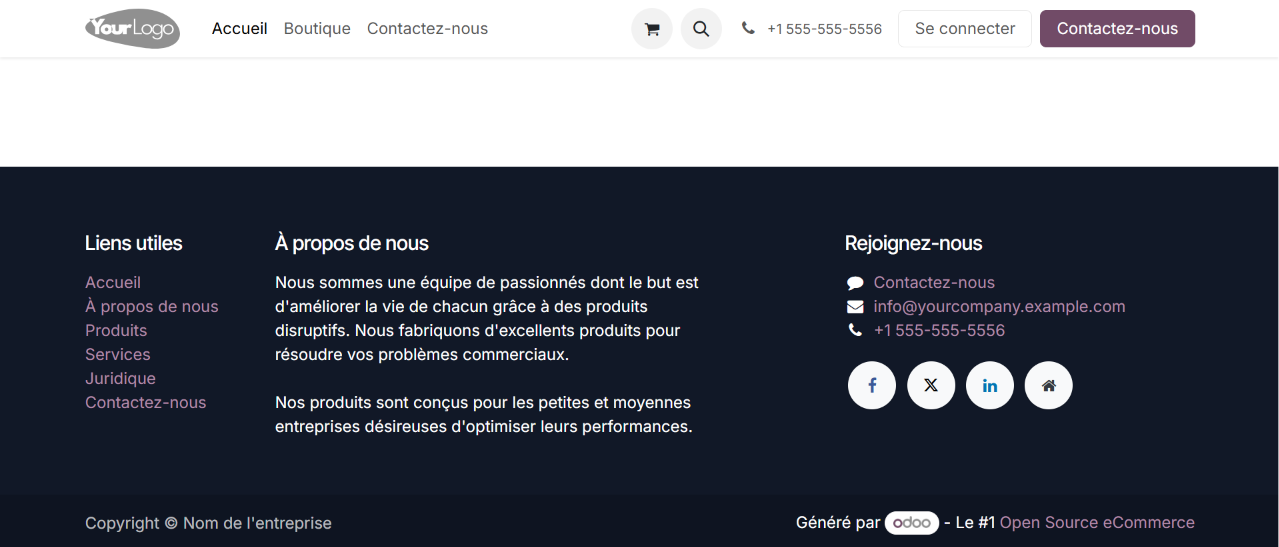
\includegraphics[width=\linewidth]{image/siteweb/Pageweb1.png}
\caption{Page d'accueil du site web}
\label{fig:pageweb1}
\end{figure}

Depuis la page d'accueil, l'utilisateur peut accéder à la rubrique \textbf{Boutique}, qui regroupe l'ensemble des offres disponibles.

\begin{figure}[H]
\centering
\includegraphics[width=\linewidth]{image/siteweb/Pageweb2.png}
\caption{Accès à la boutique}
\label{fig:pageweb2}
\end{figure}

La boutique affiche les différents produits (séjours) ainsi que leurs éventuelles variantes, permettant aux visiteurs de consulter l'ensemble des offres commercialisées.

\begin{figure}[H]
\centering
\includegraphics[width=\linewidth]{image/siteweb/Pageweb3.png}
\caption{Produits et variantes disponibles sur la boutique}
\label{fig:pageweb3}
\end{figure}

\subsection*{Publication d'un produit sur le site web}

La publication d'un produit sur le site web est réalisée depuis le module \textbf{Ventes} d'Odoo.

\begin{figure}[H]
\centering
\includegraphics[width=\linewidth]{image/siteweb/Pageweb4.png}
\caption{Accès au module Ventes}
\label{fig:pageweb4}
\end{figure}

Dans le menu \textbf{Produits}, sélectionner l'option permettant d'afficher la liste des produits.

\begin{figure}[H]
\centering
\includegraphics[width=\linewidth]{image/siteweb/Pageweb5.png}
\caption{Menu Produits}
\label{fig:pageweb5}
\end{figure}

La liste de tous les produits enregistrés dans le système est alors affichée.

\begin{figure}[H]
\centering
\includegraphics[width=\linewidth]{image/siteweb/Pageweb6.png}
\caption{Liste des produits}
\label{fig:pageweb6}
\end{figure}

Sélectionner ensuite le produit à publier.

\begin{figure}[H]
\centering
\includegraphics[width=\linewidth]{image/siteweb/Pageweb7.png}
\caption{Sélection d'un produit}
\label{fig:pageweb7}
\end{figure}

Dans la fiche produit, accéder à l'onglet \textbf{Vente}.

\begin{figure}[H]
\centering
\includegraphics[width=\linewidth]{image/siteweb/Pageweb8.png}
\caption{Onglet Vente de la fiche produit}
\label{fig:pageweb8}
\end{figure}

L'option \textbf{Publié} permet de contrôler la visibilité du produit sur le site web. En cochant cette case, le produit devient immédiatement visible dans la boutique en ligne. À l'inverse, en la décochant, le produit est retiré du site tout en restant enregistré dans Odoo.

\begin{figure}[H]
\centering
\includegraphics[width=\linewidth]{image/siteweb/Pageweb9.png}
\caption{Publication d'un produit sur le site web}
\label{fig:pageweb9}
\end{figure}
\section{VENTE DIRECTE EN LIGNE}

Le module \textbf{Website/eCommerce} d'Odoo permet aux clients d'effectuer directement leurs réservations en ligne. Les visiteurs peuvent sélectionner les produits souhaités, choisir les variantes disponibles (dates de départ, taille du groupe, type d'hébergement, etc.), puis finaliser leur commande grâce à un paiement sécurisé. Cette fonctionnalité repose sur la gestion native des variantes d'articles ainsi que sur l'intégration standard avec plusieurs fournisseurs de paiement tels que Stripe, PayPal ou Adyen.

Pour configurer un fournisseur de paiement, accéder au module \textbf{Site Web}.

\begin{figure}[H]
\centering
\includegraphics[width=\linewidth]{image/siteweb/Pageweb10.png}
\caption{Accès au module Site Web}
\label{fig:pageweb10}
\end{figure}

Depuis le menu \textbf{Configuration}, sélectionner l'option \textbf{Fournisseurs de paiement}.

\begin{figure}[H]
\centering
\includegraphics[width=\linewidth]{image/siteweb/Pageweb11.png}
\caption{Menu Configuration}
\label{fig:pageweb11}
\end{figure}



\begin{figure}[H]
\centering
\includegraphics[width=\linewidth]{image/siteweb/Pageweb12.png}
\caption{Liste des fournisseurs de paiement}
\label{fig:pageweb12}
\end{figure}
La liste des fournisseurs de paiement disponibles est alors affichée.
\begin{figure}[H]
\centering
\includegraphics[width=\linewidth]{image/siteweb/Pageweb13.png}
\caption{Activation d'un fournisseur de paiement}
\label{fig:pageweb13}
\end{figure}
Il suffit ensuite d'activer le fournisseur de paiement souhaité (par exemple Stripe, PayPal ou Adyen), puis de renseigner les informations de configuration demandées (identifiants, clés API, mode test ou production, etc.) afin de permettre le paiement sécurisé des commandes passées sur le site web.
\section{ESPACE CLIENT}

L'espace client d'Odoo, disponible nativement et sans coût supplémentaire, permet aux clients d'accéder à un portail sécurisé afin de consulter l'historique de leurs documents (devis, commandes, factures, bons de livraison, projets et tâches). Ils peuvent également télécharger leurs documents, tels que leur carnet de voyage, consulter leurs factures et effectuer le règlement du solde lorsque le paiement en ligne est configuré.

Pour accéder à cet espace, l'utilisateur se connecte d'abord au site web.

\begin{figure}[H]
\centering
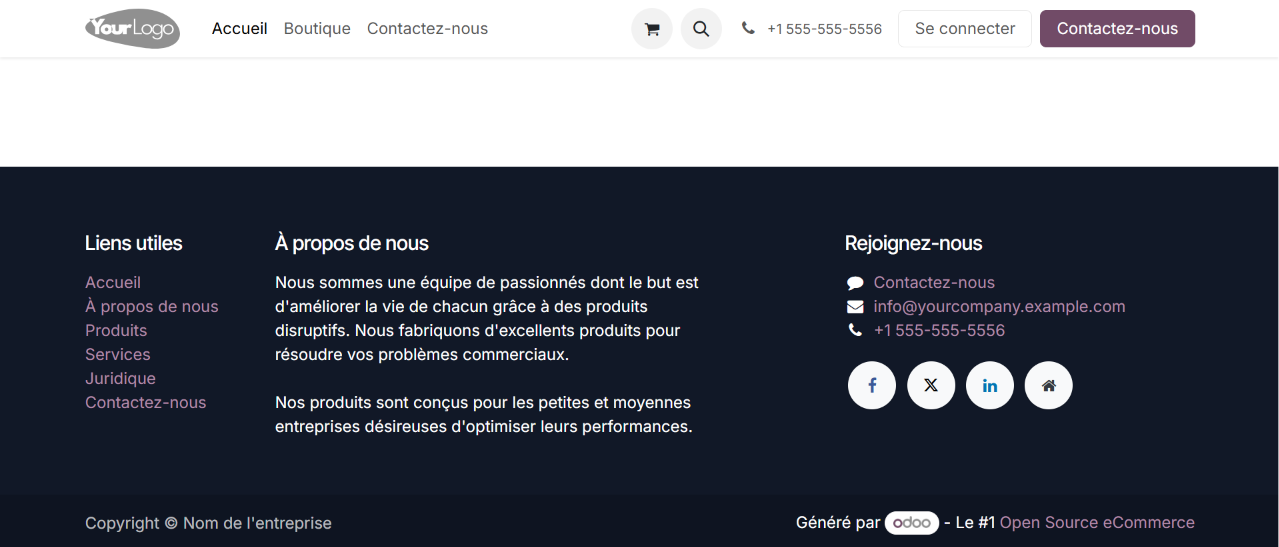
\includegraphics[width=\linewidth]{image/siteweb/Pageweb1.png}
\caption{Connexion au site web}
\label{fig:pageweb14}
\end{figure}

Une fois connecté, il clique sur son nom d'utilisateur situé en haut à droite de la page, puis sélectionne l'option \textbf{Mon compte}.

\begin{figure}[H]
\centering
\includegraphics[width=\linewidth]{image/siteweb/Pageweb14.png}
\caption{Accès à l'espace client}
\label{fig:pageweb15}
\end{figure}

Le portail client affiche ensuite un tableau de bord permettant de consulter les différents documents associés au compte, notamment les commandes, les factures, les projets et les tâches.

\begin{figure}[H]
\centering
\includegraphics[width=\linewidth]{image/siteweb/Pageweb15.png}
\caption{Tableau de bord du portail client}
\label{fig:pageweb16}
\end{figure}


%=================================================
% MODULE RESSOURCE HUMAINE
%=================================================
\chapter{Module RESSOURCE HUMAINE}
\section{Gestion des accompagnateurs}

Ce module permet la planification centralisée des activités, la gestion des congés et le suivi des disponibilités des guides accompagnateurs locaux.

\subsection{Planification des activités}

Pour planifier une activité :

\begin{enumerate}
    \item Accéder au module \textbf{Calendrier}.
    \begin{figure}[H]
\centering
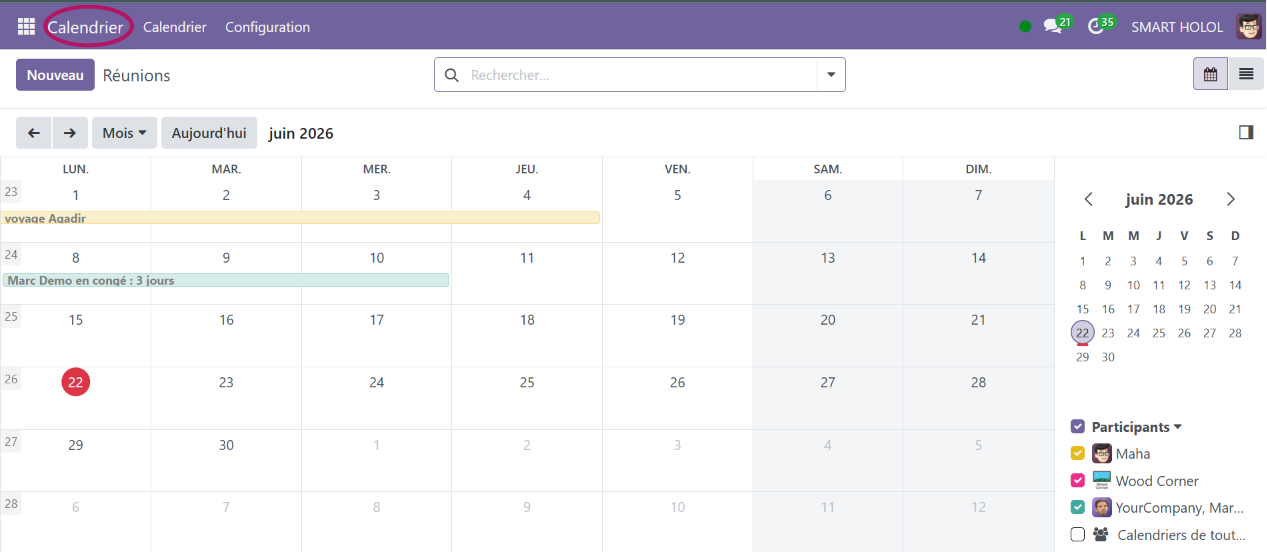
\includegraphics[width=\linewidth]{image/RH/calandrier.png}
\caption{Module Calendrier}
\label{fig:calendrier}
\end{figure}
    \item Cliquer sur la date souhaitée.
     \begin{figure}[H]
\centering
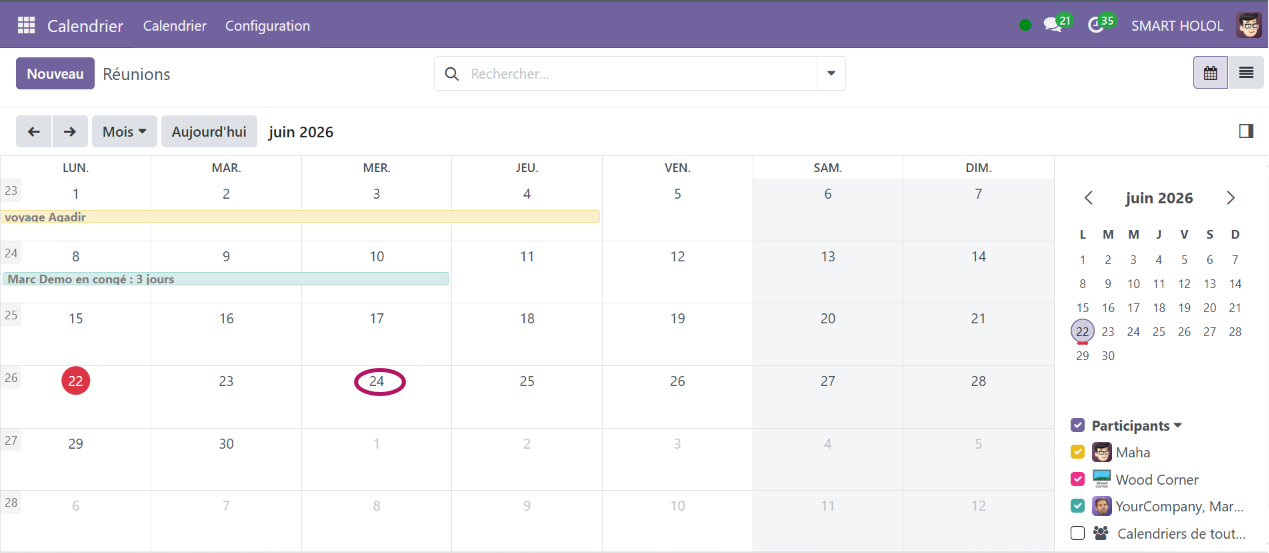
\includegraphics[width=\linewidth]{image/RH/calandrie2.png}
\caption{Module Calendrier}
\label{fig:calendrier}
\end{figure}
    \item Renseigner les informations de l'activité à planifier.
     \begin{figure}[H]
\centering
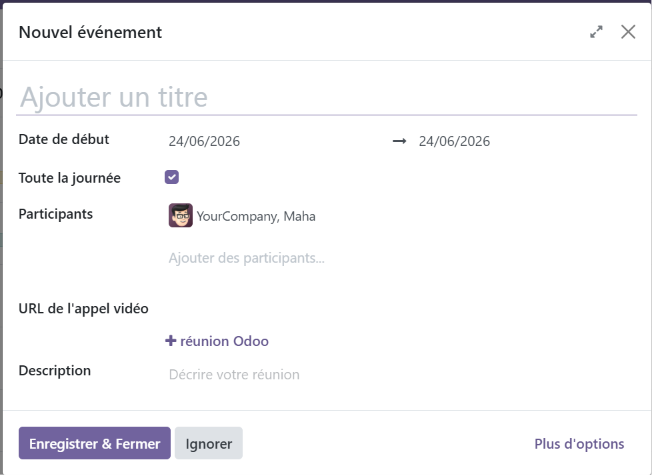
\includegraphics[width=\linewidth]{image/RH/calandrie3.png}
\caption{Module Calendrier}
\label{fig:calendrier}
\end{figure}
    \item Enregistrer la planification.
     \begin{figure}[H]
\centering
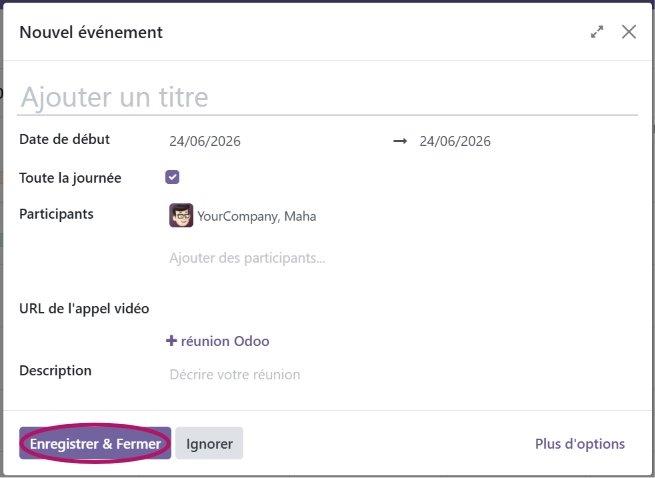
\includegraphics[width=\linewidth]{image/RH/calandrie4.png}
\caption{Module Calendrier}
\label{fig:calendrier}
\end{figure}
\end{enumerate}



\subsection{Gestion des congés}

Pour enregistrer une demande de congé :

\begin{enumerate}
    \item Accéder au module \textbf{Congés}.
    \item Cliquer sur \textbf{Nouveau}.
    \begin{figure}[H]
\centering
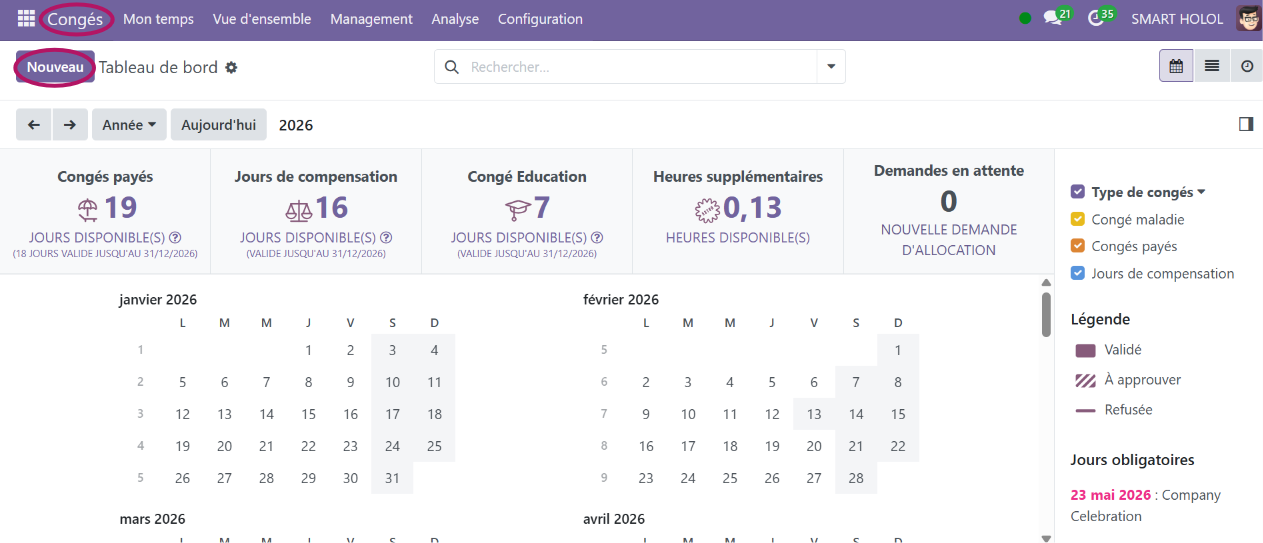
\includegraphics[width=\linewidth]{image/RH/congee.png}
\caption{Module Congés}
\label{fig:module_conge}
\end{figure}
    \item Sélectionner le type de congé souhaité.
    \begin{figure}[H]
\centering
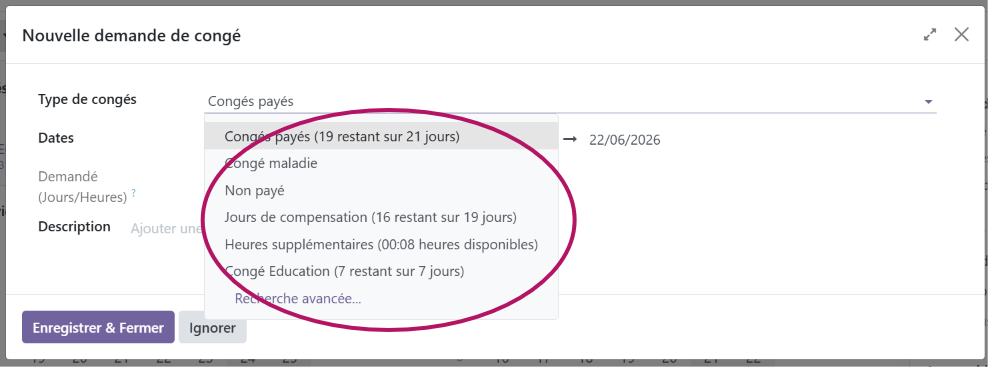
\includegraphics[width=\linewidth]{image/RH/choisir_type_ccongee.png}
\caption{Sélection du type de congé}
\label{fig:type_conge}
\end{figure}
    \item Remplir le formulaire de demande.
    \item Valider la demande.
    \begin{figure}[H]
\centering
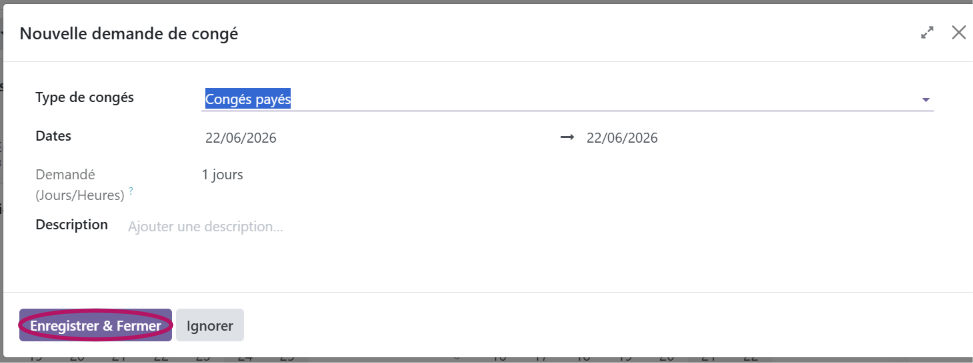
\includegraphics[width=\linewidth]{image/RH/remplir_formulaire.png}
\caption{Formulaire de demande de congé}
\label{fig:formulaire_conge}
\end{figure}
    
\end{enumerate}
\section{Gestion des notes de frais terrain}

Le module \textbf{Dépenses} permet aux accompagnateurs et aux employés de déclarer les frais engagés lors des missions terrain, tels que les frais de transport, d'hébergement, de restauration ou toute autre dépense professionnelle. Ces demandes sont ensuite soumises à validation avant remboursement.

\subsection{Création d'une note de frais}

Pour enregistrer une nouvelle dépense :

\begin{enumerate}
\item Accéder au module \textbf{Dépenses}.
\item Cliquer sur le bouton \textbf{Nouveau}.
\end{enumerate}

\begin{figure}[H]
\centering
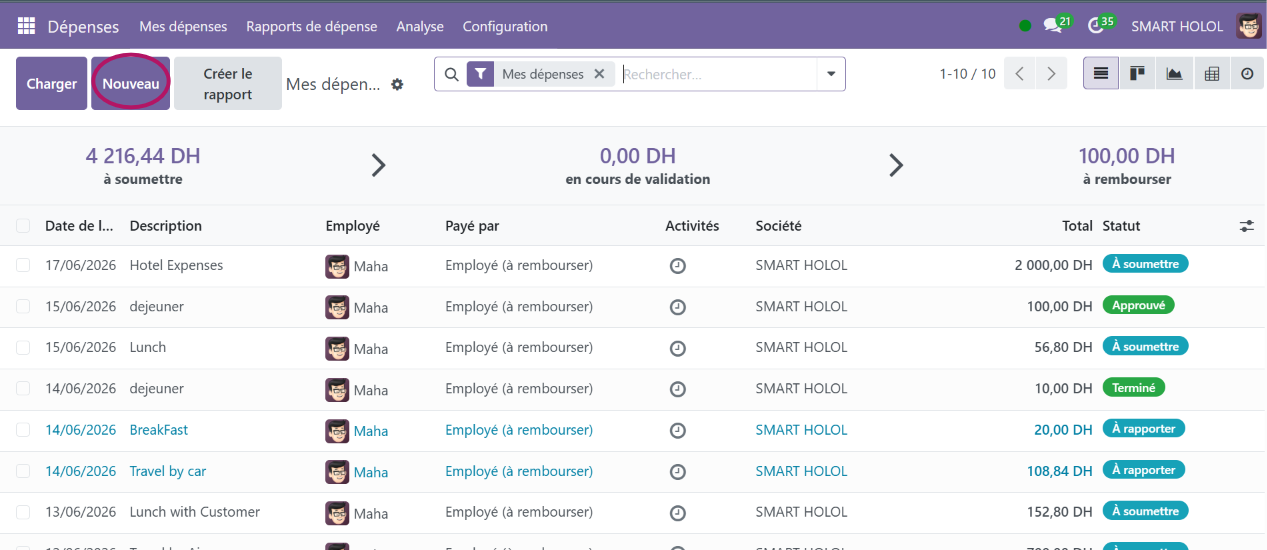
\includegraphics[width=\linewidth]{image/RH/depense1.png}
\caption{Création d'une nouvelle dépense}
\label{fig:nouvelle_depense}
\end{figure}

\subsection{Saisie des informations de la dépense}

Après avoir créé une nouvelle dépense, il est nécessaire de renseigner les informations demandées dans le formulaire :

\begin{itemize}
\item La description de la dépense ;
\item La catégorie de dépense ;
\item Le montant engagé ;
\item La date de la dépense ;
\item Le projet ou l'activité concernée ;
\item Le justificatif (facture, ticket de caisse ou reçu) si nécessaire.
\end{itemize}

Une fois les informations complétées, cliquer sur \textbf{Enregistrer} afin de soumettre la note de frais.

\begin{figure}[H]
\centering
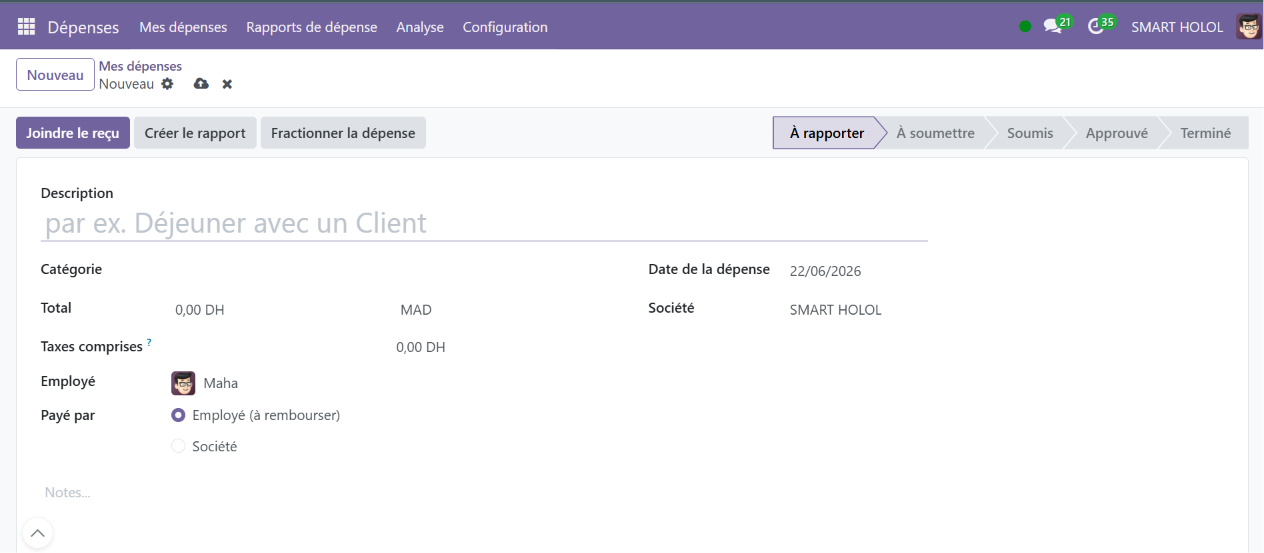
\includegraphics[width=\linewidth]{image/RH/depense2.png}
\caption{Formulaire de saisie d'une note de frais}
\label{fig:formulaire_depense}
\end{figure}

\subsection{Validation et remboursement}

Après soumission, la note de frais suit le processus de validation défini dans Odoo. Le responsable concerné peut approuver ou refuser la demande après vérification des informations et des justificatifs fournis.

Une fois validée, la dépense est intégrée au suivi comptable de l'entreprise et peut être remboursée à l'employé selon les procédures internes en vigueur.




%=================================================
% CONCLUSION
%=================================================
\chapter*{Conclusion Générale}
\addcontentsline{toc}{chapter}{Conclusion Générale}

La réalisation de cette solution marque une étape significative dans l'optimisation des flux opérationnels au sein de \textbf{Smart Holol}. L'intégration réussie de la "Grille Fonctionnelle" démontre la pertinence des choix architecturaux effectués pour répondre avec précision aux besoins métiers identifiés, tout en offrant une structure robuste et évolutive.

Au-delà de la mise en service technique, ce projet pose les fondements d'une gestion automatisée et centralisée, essentielle pour garantir la qualité de service et la réactivité de l'entreprise. La documentation ici présente constitue désormais le référentiel technique garantissant la pérennité de ces développements et facilitant l'appropriation du système par les équipes opérationnelles.

À terme, cette solution a vocation à évoluer en fonction des nouveaux défis stratégiques de \textbf{Smart Holol}. Les perspectives de développement restent ouvertes, notamment par l'ajout de modules complémentaires ou par l'optimisation des processus existants, assurant ainsi une amélioration continue de l'écosystème numérique mis en place.

\end{document}
